\documentclass[12pt]{article}
\usepackage{frankstyle}

\begin{document}

\title{A Generalized Focused Information Criterion for GMM with Applications to Panel Data Models\footnote{We thank Manuel Arellano, Otilia Boldea, Bruce Hansen, Frank Kleibergen, and seminar participants at the 2013 Latin American Workshop in Econometrics, UPenn, Tilburg, the Tinbergen Institute, and the University of Wisconsin for helpful comments and suggestions.}}

\author{Minsu Chang \hspace{1em} Francis J.\ DiTraglia\footnote{Corresponding Author:
\href{mailto:fditra@sas.upenn.edu}{\texttt{fditra@sas.upenn.edu}}, \emph{3718 Locust Walk, Philadelphia, PA 19104}}
\\ University of Pennsylvania}

\date{\footnotesize This Version: \today \hspace{0.5em} First Version: February 15, 2013}

\maketitle 
\begin{abstract}
	%!TEX root = main.tex
In this paper we propose a novel criterion for simultaneous GMM model and moment selection: the generalized focused information criterion (GFIC). 
Rather than attempting to identify the correct specification, the GFIC chooses from a set of potentially mis-specified overidentifying and parameter restrictions to minimize the mean-squared error of a target parameter specified by the user. 
Both the focused moment selection criterion (FMSC) of \cite{DiTraglia2012} and the focused information criterion (FIC) of \cite{ClaeskensHjort2003} can be viewed as special cases of the GFIC. 
In addition to the general theory, we specialize the GFIC to a simple dynamic panel model with correlated individual effects. 
In a simulation study based on this example, the GFIC performs well relative to alternatives from the literature.



	\bigskip
	\noindent\textbf{Keywords:} 
  Model Selection, Moment selection, Model averaging, Panel Data, GMM Estimation, Focused Information Criterion, Post-selection estimators

	\medskip
	\noindent\textbf{JEL Codes:} C23, C52 
\end{abstract}

%Body of the paper
%!TEX root = main.tex
\section{Introduction}

An econometric model is a tool for answering a particular research question: different questions may suggest different models for the same data. 
And the fact that a model is wrong, as the old saying goes, does not prevent it from being useful. 
This paper proposes a novel selection criterion for GMM estimation that takes both of these points to heart: the generalized focused information criterion (GFIC). 
Rather than attempting to identify the correct specification, the GFIC chooses from a set of potentially mis-specified moment conditions and parameter restrictions to yield the smallest mean squared error (MSE) estimator of a user-specified scalar target parameter. 
We derive the GFIC under local mis-specification, using asymptotic mean squared error (AMSE) to approximate finite-sample MSE. 
In this framework mis-specification, while present for any fixed sample size, disappears in the limit so that asymptotic variance and squared bias remain comparable. 
GMM estimators remain consistent under local mis-specification but their limit distributions show an asymptotic bias. 
Adding an additional moment condition or imposing a parameter restriction generally reduces asymptotic variance but, if incorrectly specified, introduces a source of bias.
The GFIC trades off these two effects in the first-order asymptotic expansion of an estimator to approximate its finite sample behavior.

The GFIC takes its motivation from a situation that is common in empirical practice.
A researcher who hopes to estimate a parameter of interest $\mu$ must decide which assumptions to use.
On the one hand is a set of relatively uncontroversial ``baseline'' assumptions.
We suppose that the baseline assumptions are correct and identify $\mu$.
But the very fact that the baseline assumptions do not raise eyebrows suggests that they may not be especially informative about $\mu$. 
On the other hand are one or more stronger controversial ``suspect'' assumptions.
These stronger assumptions are expected to be much more informative about $\mu$.
If we were certain that they were correct, we would definitely choose to impose them in estimation.
Indeed, by continuity, even if they were \emph{nearly} correct, imposing the suspect assumptions could yield a favorable bias-variance tradeoff.
This is the essential idea behind the GFIC.
When the baseline assumptions identify the model, the GFIC provides an asymptotically unbiased estimator of AMSE.

The GFIC is an extension of the focused moment selection criterion (FMSC) of \cite{DiTraglia2016}.
While the FMSC considers the problem of selecting moment conditions while holding the model specification \emph{fixed}, the GFIC allows us to select over both aspects of our specification simultaneously.
This extension is particularly valuable in panel data applications, where we may, for example, wish to carry out selection over the lag specification as well as the exogeneity assumptions used to estimate a dynamic panel model.
We specialize the GFIC to such a dynamic panel example below, and provide simulation evidence of its performance.
Online Appendix \ref{sec:additional} provides two additional examples: selecting between random and fixed effects estimators, and choosing between pooled OLS and mean-group estimators of an average effect in the presence of heterogeneity.  
In addition to extending the FMSC to a broader class of problems, we also extend the results of \cite{DiTraglia2016} on post-selection and moment-average estimators to the more general setting of the GFIC.  
%In the random versus fixed effects example, we further derive an averaging estimator that optimally combines the information contained in the two specifications.\footnote{Although we are unaware of any other proposal for averaging fixed and random effects estimator, our general approach to averaging is shared by \cite{hjort2003frequentist} and is related to \cite{hansen2017stein}.} 
%The GFIC performs well in simulations for our dynamic panel example.
We conclude with an empirical example modelling the price elasticity of cigarette demand. 

As its name suggests, the GFIC is related to the focused information criterion (FIC) of \cite{ClaeskensHjort2003}, a model selection procedure for maximum likelihood estimators that uses local mis-specification to approximate the MSE of a target parameter. 
%The idea of targeted, risk-based model selection has proved popular in recent years, leading to a number of interesting extensions. 
%\cite{HjortClaeskens2006}, for example, propose an FIC for the Cox proportional hazards model while \cite{ClaeskensCarroll} extend the FIC more generally to problems in which the likelihood involves an infinite-dimensional parameter but selection is carried out over the parametric part. 
%More recently, \cite{ZhangLiang} extend the FIC to generalized additive partially linear models and \cite{BehlClaeskensDette} develop an FIC for quantile regression.
%While MSE is a natural risk-function for asymptotically normal estimators, different applications of model selection may call for different risk functions. \cite{ClaeskensCroux2006}, for example, suggest combining local mis-specification with $L_p$-risk or mis-classification error rates to derive an FIC better-suited to prediction in logistic regression models. 
%In a similar vein, the weighted FIC (wFIC) of \cite{ClaeskensHjort2008} provides a potentially important tool for policy analysis, allowing researchers to choose the model that minimizes weighted average risk for generalized linear models. 
%While the FIC can be used, for example, to choose the best model for estimating the mean response at a given set of covariate values, the wFIC allows us to minimize the expected mean response over a \emph{distribution} of covariate values corresponding to some target population.
%In time series problems, predictive MSE is typically more interesting than estimator MSE.
%Accordingly, \cite{ClaeskensCroux} develop an FIC to minimize forecast MSE in autoregressive models where the true order of the process is infinite. 
%Independently of the FIC literature, \cite{Schorfheide2005} likewise uses local mis-specification to suggest a procedure for using finite order vector autoregressions to forecast an infinite-order vector moving average process with minimum quadratic loss. 
%This idea shares similarities with \cite{Skouras2001}.
Like the FIC and related proposals, e.g.\ \cite{Schorfheide2005}, the GFIC uses local mis-specification to derive a risk-based selection criterion.
Unlike them, however, the GFIC provides both moment and model selection for general GMM estimators. 
If the moment conditions used in estimation are the score of a maximum likelihood model and we consider model selection only, then the GFIC reduces to the FIC.
Thus, the GFIC extends both the FIC and the FMSC of \cite{DiTraglia2016}.
Comparatively few papers propose criteria for simultaneous GMM model and moment selection under mis-specification.\footnote{See \cite{Smith1992} for an approach to GMM model selection based on non-nested hypothesis testing. For a detailed discussion of the literature on moment selection, see \cite{DiTraglia2016}.} \cite{AndrewsLu} propose a family of selection criteria by adding appropriate penalty and ``bonus'' terms to the J-test statistic, yielding analogues of AIC, BIC, and the Hannan-Quinn information criterion.
\cite{HongPrestonShum} extend this idea to generalized empirical likelihood (GEL). 
The principal goal of both papers is consistent selection: they state conditions under which the correct model and all correct moment conditions are chosen in the limit. 
As a refinement to this approach, \cite{LaiSmallLiu} suggest a two-step procedure: first consistently eliminate incorrect models using an empirical log-likelihood ratio criterion, and then select from the remaining models using a bootstrap covariance matrix estimator. 
The point of the second step is to address a shortcoming in the standard limit theory. 
While first-order asymptotic efficiency requires that we use all available correctly specified moment conditions, this can lead to a deterioration in finite sample performance if some conditions are only weakly informative.
\cite{HallPeixe2003} make a similar point about the dangers of including ``redundant'' moment conditions while \cite{Caner2009} proposes a lasso-type GMM estimator to consistently remove redundant parameters.


In contrast to these suggestions, the GFIC does not aim to identify the correct model and moment conditions: its goal is a low MSE estimate of a quantity of interest, even if this entails using a specification that is not exactly correct.  
As such, the GFIC is an ``efficient'' rather than a consistent selection criterion.
There is an unavoidable trade-off between consistent selection and estimators with desirable risk properties \citep{Yang2005}.
Indeed, the worst-case risk of any consistent selection procedure is \emph{unbounded} as sample size tends to infinity \citep{LeebPoetscher2008}.
In this sense, the fact that the GFIC is not consistent is a benefit rather than a liability.
As we show in simulations below, its worst-case performance is much better than that of competing selection procedures.

Although not strictly a selection procedure, the combined moments (CM) estimator of \cite{JudgeMittelhammer} takes a similar perspective to that of the GFIC, emphasizing that incoporating the information from an incorrect specification could lead to a favorable bias-variance tradeoff under the right circumstances. 
%Their proposal uses a Cressie-Read divergence measure to combine the information from competing moment specifications, for example OLS versus two-stage least squares, yielding a data-driven compromise estimator. 
Unlike the GFIC, however, the CM estimator is not targeted to a particular research goal.
A key point of the GFIC is that two researchers using the same dataset but interested in different target parameters may find it optimal, in a minimum MSE sense, to choose different model specifications.  
We explore this idea further in our dynamic panel example below.

The remainder of this paper is organized as follows. Section \ref{sec:asymp} derives the asymptotic distribution of GMM estimators under locally mis-specified moment conditions and parameter restrictions. 
Section \ref{sec:GFIC} uses this information to calculate the AMSE of a user-specified target parameter and provides asymptotically unbiased estimators of the required bias parameters, yielding the GFIC. 
Section \ref{sec:avg} extends the results on averaging estimators and post-selection inference from \cite{DiTraglia2016} to the more general setting of this paper.
Section \ref{sec:Dpanel} specializes the GFIC to a dynamic panel example, and Section \ref{sec:Dpanel_sim} presents simulation results.
Finally, Section \ref{sec:cigarettes} presents our empirical example and  Section \ref{sec:conclude} concludes.  
Proofs and supplementary simulation results appear in the Appendix.
Further examples and simulation results appear in Online Appendices \ref{sec:additional} and \ref{sec:simulation_supplement}.


%!TEX root = main.tex
\section{Asymptotic Framework}
\label{sec:asymp}
Let $f(\cdot, \cdot)$ be a $(p+q)$-vector of moment functions of a random vector $Z$ and an $(r+s)$-dimensional parameter vector $\beta$.
To represent moment selection, we partition the moment functions according to $f(\cdot,\cdot) = \left(g(\cdot, \cdot)', h(\cdot, \cdot)'\right)'$ where $g(\cdot, \cdot)$ and $h(\cdot, \cdot)$ are $p$- and $q$-vectors.
The moment condition associated with $g(\cdot, \cdot)$ is assumed to be correct, while that associated with $h(\cdot,\cdot)$ is locally mis-specified.  
The moment selection problem is to choose which, if any, of the elements of $h$ to use in estimation. 
To represent model selection, we partition the full parameter vector according to $\beta = \left(\gamma', \theta'\right)'$, where $\gamma$ is an $r$-vector and $\theta$ an $s$-vector of parameters.
The model selection problem is to decide which if any of the elements of $\gamma$ to estimate, and which to set equal to the corresponding elements of $\gamma_0$, an $r$-vector of known constants.
The parameters contained in $\theta$ are those that we always estimate, the ``protected'' parameters.
Any specification that does not estimate the full parameter vector $\beta$ is locally mis-specified.
The precise form of the local mis-specification, over parameter restrictions and moment conditions, is as follows.

\begin{assump}[Local Mis-specification]
\label{assump:local}
Let $\{Z_{ni}\colon 1\leq i \leq n, n =1, 2, \hdots\}$ be an iid triangular array of random vectors defined on a probability space $(\Upsilon, \mathcal{F},P)$ satisfying
	\begin{enumerate}[(a)]
    \item $E[g(Z_{ni}, \gamma_n,\theta_0)]=0$, with $\gamma_n = \gamma_0 + n^{-1/2} \delta$
    \item $E[h\left( Z_{ni}, \gamma_n, \theta_0\right)] = \tau_n$, with $\tau_n = n^{-1/2} \tau$
		\item $\{f(Z_{ni}, \gamma_n, \theta_0)\colon 1\leq i \leq n, n = 1, 2, \hdots \}$ is uniformly integrable, and 
		\item $Z_{ni}\overset{d}{\rightarrow} Z_i$.
	\end{enumerate}
	where $\gamma_0$ is a (known) $r$-vector of parameter restrictions, $\delta$ an unknown $r$-vector of constants, and $\tau$ an unknown $q$-vector of constants.
\end{assump}

Assumption \ref{assump:local} specifies a triangular array data generating process in which the the true parameter vector $\beta_n = \left(\gamma_n', \theta_0' \right)'$, changes with sample size but converges to $\beta_0 = \left(\gamma_0', \theta_0'\right)'$ as $n\rightarrow \infty$.\footnote{For simplicity, and because it is the case for all examples we consider below, we assume that the triangular array from Assumption \ref{assump:local} is iid within each row. Note however, that the $Z_{ni}$ are not iid \emph{across} rows: $\gamma_n$ and $\tau_n$ change with $n$. As such, the triangular array machinery is still required to describe our results.}
Unless some elements of $\delta$ are zero, any estimator that restricts $\gamma$ is mis-specified for fixed $n$. 
In the limit, however, the restriction $\gamma = \gamma_0$ holds. 
Similarly, for any fixed sample size $n$, the expectation of $h$ evaluated at the true parameter value $\beta_n$ depends on the unknown constant vector $\tau$, but this source of mis-specification disappears in the limit. 
Thus, under Assumption \ref{assump:local}, only estimators that use moment conditions from $g$ to estimate the full parameter vector $\beta$ are correctly specified. 
In the limit, however, \emph{every} estimator is correctly specified, regardless of which elements of $\gamma$ it restricts and which elements of $h$ it includes. 
The purpose of local mis-specification is to ensure that squared asymptotic bias is of the same order as asymptotic variance: Assumption \ref{assump:local} is a device rather than literal description of real-world data. 
Note that, by Assumption \ref{assump:local}, the limiting random variable $Z_i$ satisfies the population moment condition $E[f\left(Z_i,\gamma_0, \theta_0\right)]=0$. 
Since the $Z_i$ are assumed to have a common marginal law, we will use the shorthand $Z$ for $Z_i$ throughout.
Accordingly, define:
		\begin{equation}F  =  \left[\begin{array}{cc}  \nabla_{\gamma'}g\left(Z,\gamma_0, \theta_0\right) &   \nabla_{\theta'}g\left(Z,\gamma_0, \theta_0\right) \\
 \nabla_{\gamma'}h\left(Z,\gamma_0, \theta_0\right)  &   \nabla_{\theta'}h\left(Z,\gamma_0, \theta_0\right)  
		 \end{array}\right] = \left[\begin{array}{cc}F_\gamma & F_\theta \end{array}\right] = 
		  \left[\begin{array}{cc} G_\gamma & G_\theta \\
					 H_\gamma& H_\theta
		 \end{array}\right] = \left[\begin{array}{c} G\\ H \end{array}\right]
	\end{equation}
along with 
	\begin{equation}
		\Omega = Var\left[ \begin{array}{c} g(Z, \gamma_0, \theta_0) \\ h(Z, \gamma_0, \theta_0) \end{array}\right] =\left[ \begin{array}{cc}\Omega_{gg} & \Omega_{gh}\\ \Omega_{hg}& \Omega_{hh} \end{array} \right].
	\end{equation}
Each of these expressions involves the limiting random variable $Z$ rather than $Z_{ni}$. 
Thus, the corresponding expectations are taken with respect to a distribution for which all moment conditions have expectation zero  evaluated at $(\gamma_0,\theta_0)$.
Finally, let $F(b,c) = \Xi_c F \Xi_b'$ and $\Omega_c = \Xi_c \Omega \Xi_c'$ and $W_c = \Xi_c W \Xi_c'$ where $W$ is the positive definite probability limit of $\widetilde{W}$. 

Before defining the estimators under consideration, we require some further notation. Let $b$ be a \emph{model selection vector}, an $r$-vector of ones and zeros indicating which elements of $\gamma$ we have chosen to estimate. 
When $b = 1_r$, where $1_m$ represents an $m$-vector of ones, we estimate both $\theta$ and the full vector $\gamma$. 
When $b = 0_r$, where $0_m$ denotes an $m$-vector of zeros, we estimate only $\theta$, setting $\gamma=\gamma_0$. 
More generally, we estimate $|b|$ components of $\gamma$ and set the others equal to the corresponding elements of $\gamma_0$. 
Let $\gamma^{(b)}$ be the $|b|$-dimensional subvector of $\gamma$ corresponding to those elements selected for estimation. 
Similarly, let $\gamma^{(-b)}_0$ denote the $(r-|b|)$-dimensional subvector containing the values to which we set those components of $\gamma$ that are \emph{not} estimated.
Analogously, let $c=\left(c_g', c_h'\right)'$ be a \emph{moment selection vector}, a $(p+q)$-vector of ones and zeros indicating which of the moment conditions we have chosen to use in estimation. 
We denote by $|c|$ the total number of moment conditions used in estimation. 
Let $\mathcal{BC}$ denote the collection of all model and moment selection pairs $(b,c)$ under consideration.


To express moment and model selection in matrix form, we define the selection matrices $\Xi_b$ and $\Xi_c$.
Multiplying $\beta$ by the $(|b| + s)\times(r+s)$ \emph{model selection matrix} $\Xi_b$ extracts the elements corresponding to $\theta$ and the subset of $\gamma$ indicated by the model selection vector $b$. 
Thus $\Xi_b \beta = \left(\gamma^{(b)'}, \theta' \right)'$.
Similarly, multiplying a vector by the $|c|\times(p+q)$ moment selection matrix $\Xi_c$ extracts the components corresponding to the moment conditions indicated by the moment selection vector $c$. 

To express the estimators themselves, define the sample analogue of the expectations in Assumption \ref{assump:local} as follows,
\begin{equation}
	f_n(\beta) = \frac{1}{n}\sum_{i=1}^n f(Z_{ni}, \gamma, \theta) = \left[\begin{array}{c}g_n(\beta)\\ h_n(\beta) \end{array} \right] = \left[\begin{array}{c} n^{-1}\sum_{i=1}^n g(Z_{ni}, \theta, \gamma)\\n^{-1}\sum_{i=1}^n h(Z_{ni}, \theta, \gamma) \end{array}\right]
\end{equation}
and let $\widetilde{W}$ be a $(p+q)\times(p+q)$ positive semi-definite weighting matrix with blocks $\widetilde{W}_{gg}, \widetilde{W}_{gh}, \widetilde{W}_{hg}$ and $\widetilde{W}_{hh}$, partitioned conformably to the partition of $f(Z,\beta)$ by $g(Z,\beta)$ and $h(Z,\beta)$. 
Each model and moment selection pair $(b,c)\in \mathcal{BC}$ defines a $(|b|+s)$-dimensional estimator $\widehat{\beta}(b,c)=( \widehat{\gamma}^{(b)}(b,c)',\widehat{\theta}(b,c)')'$ of $\beta^{(b)}= \left(\gamma^{(b)'}, \theta'  \right)'$ according to
	\begin{equation}
    \widehat{\beta}(b,c) = \underset{\beta^{(b)}\in \mathbf{B}^{(b)}} {\mbox{arg min}}\;\left[\Xi_c f_n\left(\beta^{(b)}, \gamma_0^{(-b)}\right)\right]'\left[\Xi_c \widetilde{W}\Xi_c' \right]\left[\Xi_c f_n\left(\beta^{(b)}, \gamma_0^{(-b)}\right)\right].
	\end{equation}


We now state a number of standard high-level regularity conditions that will be assumed throughout our derivations below.

\begin{assump}[High-level Regularity Conditions]
  \label{assump:high-level}
    \mbox{}
\begin{itemize}
\item[(a)] $\beta_0$ lies in the interior of $\Theta$, a compact set
\item[(b)] $\widetilde{W} \rightarrow_{p} W$, a positive definite matrix
\item[(c)] $W_c \Xi_c E[f(Z, \beta)] = 0$ if and only if $\beta = \beta_0$, where $W_c = \Xi_c W \Xi_c'$
\item[(d)] $E[f(Z,\beta)]$ is continuous on $\Theta$
\item[(e)] $sup_{\beta\in \Theta} ||f_n(\beta) - E[f(Z,\beta)]||\rightarrow_p 0$
\item[(f)] $f$ is Z-almost surely differentiable in an open neighborhood $\mathcal{B}$ of $\beta_0$
\item[(g)] $sup_{\beta \in \Theta} ||\nabla_{\beta} f_n(\beta) - F(\beta)|| \rightarrow_p 0 $
\item[(h)] $\sqrt{n}f_n(\beta_0) - \sqrt{n}E[f(Z,\beta_0)] \rightarrow_d \mathscr{N}$ where $\mathscr{N} \sim N_{p+q}(0,\Omega)$
\item[(i)] $F(b,c)' W_c F(b,c)$ is invertible, where $W_c = \Xi_c W \Xi_c'$
\end{itemize}
\end{assump}

  A particularly important special case is the estimator using only the moment conditions in $g$ to estimate the full parameter vector $\beta = \left(\gamma', \theta' \right)'$.
  We call this the \emph{valid} estimator and denote it by $\widehat{\beta}_v$.  
  Because it is assumed to be correctly specified both for finite $n$ and in the limit, the valid estimator contains the information we use to identify $\tau$ and $\delta$, and thus carry out moment and model selection. 
We assume that the valid estimator is identified.

\begin{assump}[GFIC Identification Condition]
  Let $\widehat{\beta}_v$ denote the GMM estimator for $\beta = \left(\gamma', \theta' \right)'$ based solely on the moment conditions contained in g:
\begin{equation}
  \widehat{\beta}_v = \left(\widehat{\gamma}_{v}', \widehat{\theta}_{v}'\right)' =\underset{\beta \in \mathbf{B}}{\mbox{arg min}}\; g_n(\beta)' \widetilde{W}_{gg} \; g_n(\beta).
\end{equation}
We call this the ``valid estimator'' and assume that it satisfies all the conditions of Assumption \ref{assump:high-level}.
In particular assume that $\widehat{\beta}_v$ is identified, which implies $p \geq r+s$.
\end{assump}

Because Assumption \ref{assump:local} ensures that they are correctly specified in the limit, \emph{all} candidate specifications $(b,c)\in \mathcal{BC}$ provide consistent estimators of $\theta_0$ under standard, high level regularity conditions (see Assumption \ref{assump:high-level}).
Essential differences arise, however, when we consider their respective asymptotic distributions. 
Under Assumption \ref{assump:local}, both $\delta$ and $\tau$ induce a bias term in the limiting distribution of $\sqrt{n}\left(\widehat{\beta}(b,c) - \beta_0^{(b)}\right)$. 

\begin{thm}[Asymptotic Distribution]
\label{thm:asymp}
Under Assumptions \ref{assump:local}--\ref{assump:high-level}
		\begin{equation}
		\sqrt{n}\left(\widehat{\beta}(b,c) - \beta_0^{(b)}\right) \overset{d}{\rightarrow} - K(b,c)\Xi_c \left(\mathscr{N}+ \left[ \begin{array}{c} 0\\ \tau\end{array}\right] - F_\gamma\delta\right)
	\end{equation}
where $\beta_0^{(b)'} = (\gamma_0^{(b)'}, \theta_0')'$, $K(b,c) = \left[F(b,c)'W_c F(b,c)\right]^{-1} F(b,c)' W_c$
and $\mathscr{N} \sim \mbox{N}(0, \Omega)$ with $\mathscr{N} = (\mathscr{N}_g', \mathscr{N}_h')'$.
\end{thm}	
Because it employs the correct specification, the valid estimator of $\theta$ shows no asymptotic bias.
Moreover, the valid estimator of $\gamma$ has an asymptotic distribution that is centered around $\delta$, suggesting an estimator of this bias parameter.
\begin{cor}[Asymptotic Distribution of Valid Estimator]
\label{cor:valid}
Under Assumptions \ref{assump:local}--\ref{assump:high-level}
		$$\sqrt{n}\left( \widehat{\beta}_v - \beta_0 \right) = \sqrt{n}\left(\begin{array}{c} \widehat{\theta}_v - \theta_0\\ \widehat{\gamma}_v - \gamma_0\end{array} \right) \overset{d}{\rightarrow}  \left[\begin{array}{c} 0\\ \delta\end{array}\right] -K_v \mathscr{N}_g$$
where $K_v = \left[G'W_{gg}G\right]^{-1}G'W_{gg}$ and $W_{gg} = \mbox{plim }\widetilde{W}_{gg}$.
\end{cor}
We use these results in the following section to construct the GFIC.


%!TEX root = main.tex
\section{The GFIC}
\label{sec:GFIC}
The GFIC chooses among potentially incorrect moment conditions and parameter restrictions to minimize estimator AMSE for a scalar target parameter. 
Denote this target parameter by $\mu = \varphi(\gamma, \theta)$, where  $\varphi$ is a real-valued, almost surely continuous function of the underlying model parameters $\theta$ and $\gamma$.
Let $\mu_n = \varphi(\gamma_n,\theta_0)$ and define $\mu_0$ and $\widehat{\mu}(b,c)$  analogously.
By Theorem \ref{thm:asymp} and the delta method, we have the following result.
\begin{cor} Under the hypotheses of Theorem \ref{thm:asymp},
		$$\sqrt{n}\left(\widehat{\mu}(b,c) - \mu_0 \right) \overset{d}{\rightarrow} -\nabla_\beta\varphi_0'\Xi_b '  K(b,c)\Xi_c \left(\mathscr{N}+ \left[ \begin{array}{c} 0\\ \tau\end{array}\right] - F_\gamma\delta\right) $$
where $\varphi_0 = \varphi(\gamma_0,\theta_0)$.
\end{cor}
The true value of $\mu$, however,  is $\mu_n$ rather than $\mu_0$ under Assumption \ref{assump:local}.
Accordingly, to calculate AMSE we recenter the limit distribution as follows.
\begin{cor} 
\label{cor:mulimit}
Under the hypotheses of Theorem \ref{thm:asymp},
		$$\sqrt{n}\left(\widehat{\mu}(b,c) - \mu_n \right) \overset{d}{\rightarrow} -\nabla_\beta\varphi_0'\Xi_b '  K(b,c)\Xi_c \left(\mathscr{N}+ \left[ \begin{array}{c} 0\\ \tau\end{array}\right] - F_\gamma\delta\right) -\nabla_\gamma \varphi_0' \delta$$
where $\varphi_0 = \varphi(\gamma_0,\theta_0)$.
\end{cor}

We see that the limiting distribution of $\widehat{\mu}(b,c)$ is not, in general, centered around zero: both $\tau$ and $\delta$ induce an asymptotic bias. 
Note that, while $\tau$ enters the limit distribution only once, $\delta$ has two distinct effects. 
First, like $\tau$, it shifts the limit distribution of $\sqrt{n}f_n(\gamma_0, \theta_0)$ away from zero, thereby influencing the asymptotic behavior of $\sqrt{n}\left(\widehat{\mu}(b,c) - \mu_0 \right)$. 
Second, unless the derivative of $\varphi$ with respect to $\gamma$ is zero at $(\gamma_0, \theta_0)$, $\delta$ induces a second source of bias when $\widehat{\mu}(b,c)$ is recentered around $\mu_n$. 
Crucially, this second source of bias exactly cancels the asymptotic bias present in the limit distribution of $\widehat{\gamma}_v$. 
Thus, the valid estimator of $\mu$ is asymptotically unbiased and its AMSE equals its asymptotic variance.
\begin{cor}
\label{cor:muvalid}
Under the hypotheses of Theorem \ref{thm:asymp},
	$$\sqrt{n}\left( \widehat{\mu}_v - \mu_n\right) \overset{d}{\rightarrow} -\nabla_\beta \varphi(\theta_0, \gamma_0)' K_v\mathscr{N}_g$$
where $\widehat{\mu}_v = \varphi(\widehat{\theta}_v,\widehat{\gamma}_v)$. Thus, the valid estimator $\widehat{\mu}_v$ shows no asymptotic bias and has asymptotic variance $\nabla_\beta \varphi(\theta_0, \gamma_0)'K_v \Omega_{gg}K_v'\nabla_\beta \varphi(\theta_0, \gamma_0)$.
\end{cor}
 
Using Corollary \ref{cor:mulimit}, the AMSE of $\widehat{\mu}(b,c)$ is as follows,
	\begin{align}
	\label{eq:AMSE}
		\mbox{AMSE}\left(\widehat{\mu}(b,c)\right) &= \mbox{AVAR}\left(\widehat{\mu}\left(b,c\right)\right)  + \mbox{BIAS}\left(\widehat{\mu}\left(b,c\right)\right)^2\\
		\mbox{AVAR}\left(\widehat{\mu}\left(b,c\right)\right) &= \nabla_\beta\varphi_0'\Xi_b '  K(b,c)\Omega_c K(b,c)'\Xi_b\nabla_\beta\varphi_0\\
		\mbox{BIAS}\left(\widehat{\mu}\left(b,c\right)\right) &= -\nabla_{\beta} \varphi_0' M(b,c)\left[\begin{array}{c} \delta \\ \tau\end{array} \right]
		\label{eq:bias}
\end{align}
where
\begin{equation}
	M(b,c) = \Xi_b'K(b,c) \Xi_c \left[\begin{array}{cc} -G_\gamma & 0 \\ -H_\gamma & I \end{array} \right] +\left[\begin{array}{ll} I_r & 0_{r\times q} \\ 0_{p\times r} & 0_{s\times q} \end{array} \right]
\end{equation}

The idea behind the GFIC is to construct an estimate $\widehat{\mbox{AMSE}}\left(\widehat{\mu}(b,c)\right)$ and choose the specification $(b^*,c^*)\in\mathcal{BC}$ that makes this quantity as small as possible. 
As a side-effect of the consistency of the estimators $\widehat{\beta}(b,c)$, the usual sample analogues provide consistent estimators of $K(b,c)$ and $F_{\gamma}' = (G_\gamma', H_\gamma')$ under Assumption \ref{assump:local}, and $\varphi(\widehat{\theta}_v,\gamma_0)$ is consistent for $\varphi_0$. 
Consistent estimators of $\Omega$ are also readily available under local mis-specification although the best choice may depend on the situation.\footnote{We discuss this in more detail for our examples in Section \ref{sec:examples} below.}
Since $\gamma_0$ is known, as are $\Xi_b$ and $\Xi_c$, only $\delta$ and $\tau$ remain to be estimated. 
Unfortunately, neither of these quantities is consistently estimable under local mis-specification. 
Intuitively, the data become less and less informative about $\tau$ and $\delta$ as the sample size increases since each term is divided by $\sqrt{n}$. 
Multiplying through by $\sqrt{n}$ counteracts this effect, but also stabilizes the variance of our estimators. 
Hence, the best we can do is to construct \emph{asymptotically unbiased} estimators of $\tau$ and $\delta$. 
Corollary \ref{cor:valid} provides the required estimator for $\delta$, namely $\widehat{\delta} = \sqrt{n}\left(\widehat{\gamma}_v - \gamma_0\right)$, while Lemma \ref{lem:tauhatasymp} provides an asymptotically unbiased estimator of $\tau$ by plugging $\widehat{\beta}_v$ into the sample analogue of the $h$-block of moment conditions.

\begin{cor} 
\label{cor:deltahat}
Under the hypotheses of Theorem \ref{thm:asymp},
	$\widehat{\delta} = \sqrt{n}\left(\widehat{\gamma}_v - \gamma_0\right) \overset{d}{\rightarrow} \delta - K_{v}^{\gamma} \mathscr{N}_g$
where 
$K_v = \left[G'W_{gg}G\right]^{-1}G'W_{gg}$.
%= \left(K_{v}^{\gamma '}, K_{v}^{\theta '}\right)'$. 
Hence, $\widehat{\delta}$ is an asymptotically unbiased estimator of $\delta$.
\end{cor} 

\begin{lem}
\label{lem:tauhatasymp}
Under the hypotheses of Theorem \ref{thm:asymp},
	$$\widehat{\tau} = \sqrt{n}h_n\left(\widehat{\beta}_v\right) \overset{d}{\rightarrow} \tau - HK_v \mathscr{N}_g + \mathscr{N}_h$$
where $K_v = \left[G'W_{gg}G\right]^{-1}G'W_{gg}$. Hence, $\widehat{\tau}$ is an asymptotically unbiased estimator of $\tau$.
\end{lem}

Combining Corollary \ref{cor:deltahat} and Lemma \ref{lem:tauhatasymp}, gives the joint distribution of $\widehat{\delta}$ and $\widehat{\tau}$.

\begin{thm}
\label{thm:jointbias}
Under the hypotheses of Theorem \ref{thm:asymp},
	\[\left[\begin{array}{c}\widehat{\delta}\\ \widehat{\tau}\end{array}\right] = \sqrt{n}\left[\begin{array}{c}\left(\widehat{\gamma}_v-\gamma_0\right)\\h_n(\widehat{\beta}_v)\end{array}\right]
  \overset{d}{\rightarrow} \left[\begin{array}{c}\delta\\ \tau\end{array} \right] +\Psi \mathscr{N}, \quad
  \Psi = \left[\begin{array}{cc} -K_{v}^\gamma&\mathbf{0} \\ -HK_v&I\end{array}\right]
\]
	where $K_v = \left[G'W_{gg}G\right]^{-1}G'W_{gg}$  is partitioned according to $K_v' = (K_v^{\gamma '}, K_v^{\theta '})$.
\end{thm}
Now, we see immediately from Equation \ref{eq:bias} that
$$\mbox{BIAS}\left(\widehat{\mu}\left(b,c\right)\right)^2 = \nabla_\beta \varphi_0' M(b,c) \left[\begin{array}{cc}  \tau \tau'& \tau \delta'\\ \delta \tau'& \delta \delta'\end{array}\right] M(b,c)' \nabla_\beta \varphi_0$$
Thus, the bias parameters $\tau$ and $\delta$ enter the AMSE expression in Equation \ref{eq:AMSE} as outer products: $\tau\tau'$, $\delta\delta'$ and $\tau\delta'$.
Although $\widehat{\tau}$ and $\widehat{\delta}$ are asymptotically unbiased estimators of $\tau$ and $\delta$, it does \emph{not} follow that $\widehat{\tau}\widehat{\tau}$, $\widehat{\delta}\widehat{\delta}$ and $\widehat{\tau}\widehat{\delta}'$ are  asymptotically unbiased estimators of $\tau\tau'$, $\delta\delta'$, and $\tau\delta'$. 
The following result shows how to adjust these quantities to provide the required asymptotically unbiased estimates. 

\begin{cor}
\label{cor:biasestimators}
Suppose that $\widehat{\Psi}$ and $\widehat{\Omega}$ are consistent estimators of $\Psi$ and $\Omega$. Then, $\widehat{B}$ is an asymptotically unbiased estimator of $B$, where
\[
  \widehat{B} = \left[\begin{array}{cc}  \widehat{\tau} \widehat{\tau}'& \widehat{\tau} \widehat{\delta}'\\ \widehat{\delta} \widehat{\tau}'& \widehat{\delta} \widehat{\delta}'\end{array}\right] - \widehat{\Psi} \widehat{\Omega} \widehat{\Psi}', \quad B = 
\left[\begin{array}{cc}  \tau \tau'& \tau \delta'\\ \delta \tau'& \delta \delta'\end{array}\right].
\]
\end{cor}
Combining Corollary \ref{cor:biasestimators} with consistent estimates of the remaining quantities yields the GFIC, an asymptotically unbiased estimator of the AMSE of our estimator of a target parameter $\mu$ under each specification $(b,c)\in \mathcal{BC}$
\begin{equation}
\mbox{GFIC}(b,c) =\nabla_\beta \widehat{\varphi}_0' \left[\Xi_b' \widehat{K}(b,c)\widehat{\Omega}_c \widehat{K}(b,c)'\Xi_b +  \widehat{M}(b,c) \;\widehat{B} \; \widehat{M}(b,c)'\right]\nabla_\beta \widehat{\varphi}_0.
\end{equation}
We choose the specification $(b^*,c^*)$ that minimizes the GFIC over the candidate set $\mathcal{BC}$. 


%!TEX root = main.tex
\section{Averaging and Post-Selection Inference}
\label{sec:avg}
While we are primarily concerned in this paper with the mean-squared error performance of our proposed selection techniques, it is important to have tools for carrying out valid inference post-selection.
To this end, we now show how to extend the results from Section 4 of \cite{DiTraglia2012} to the more general setting considered in this paper, one that allows for simultaneous model and moment selection.\footnote{Because the conceptual issues are largely the same as in the case where one considers only moment selection, we direct the reader to \cite{DiTraglia2012} for more discussion.}
Consider an estimator of the form 
	$$\widehat{\mu} = \sum_{(b,c) \in \mathcal{BC}} \widehat{\omega}(b,c) \widehat{\mu}(b,c)$$
  where $\widehat{\mu}$ denotes the target parameter under the moment conditions and parameter restrictions indexed by $(b,c)$, $\mathcal{BC}$ denotes the full set of candidate specifications, and $\widehat{\omega}(b,c)$ denotes a collection of data-dependent weights satisfying the following assumption.
\begin{assump}[Data-Dependent Weights] Let $\widehat{\omega}(b,c)$ be a function of the data $Z_{n1}, \hdots, Z_{nn}$ and $(b,c)$ satisfying
	\begin{enumerate}[(a)] 
		\item $\sum_{(b,c) \in \mathcal{BC}} \widehat{\omega}(b,c) = 1$
		\item $\widehat{\omega}(b,c) \overset{d}{\rightarrow} \psi(\mathscr{N}, \delta, \tau|b,c)$ jointly for all $(b,c) \in \mathcal{BC}$ where $\psi$ is a function of the normal random vector $\mathscr{N}$, the bias parameters $\delta$ and $\tau$, and consistently estimable quantities only.
	\end{enumerate}
\label{assump:weight}
\end{assump}

Assumption \ref{assump:weight} is quite weak, covering a broad range of examples, including genuine averaging estimators, post-GFIC estimators, and pre-test estimators based on the J-statistic.
Under this assumption, we can characterize the limit distribution of $\widehat{\mu}$ as follows.

\begin{cor}[Limit Distribution of Averaging Estimators]
Let $\widehat{\omega}(b,c)$ be a set of weights satisfying Assumption \ref{assump:weight}. Then, under the hypotheses of Theorem \ref{thm:asymp},  
	$$\sqrt{n}\left(\widehat{\mu} - \mu_n\right) \overset{d}{\rightarrow} \Lambda(\tau,\delta)$$
where
	\begin{equation}
		\Lambda(\tau,\delta) = -\nabla_\beta\varphi_0' \sum_{(b,c) \in \mathcal{BC}} \psi(\mathscr{N},\delta, \tau|b,c) \left\{\Xi_b' K(b,c) \Xi_c \mathscr{N} + M(b,c)  \left[\begin{array}{c}\delta \\ \tau \end{array} \right]\right\}
	\end{equation}
\end{cor}
Note that the limit distribution from the preceding corollary is highly non-normal: it is a \emph{randomly} weighted average of a normal random vector, $\mathscr{N}$.
To tabulate this distribution for the purposes of inference, we will in general need to resort to simulation.
If $\tau$ and $\delta$ were known, the story would end here.
We could simply substitute consistent estimators of $K$ and $M$, and then repeatedly draw $\mathscr{N} \sim N(0, \widehat{\Omega})$, where $\widehat{\Omega}$ is a consistent estimator of $\Omega$, and thus tabulate the distribution of $\Lambda$ to arbitrary precision. 
Unfortunately, no consistent estimators of $\tau$ or $\delta$ exist: all we have at our disposal are asymptotically unbiased estimators.
Simply plugging in these estimators $\widehat{\tau}$ and $\widehat{\delta}$ and proceeding with the simulation is not guaranteed to lead to valid confidence intervals.\footnote{Although it does not work in general, in particular examples this plug-in procedure may perform well. For more discussion of this point, see Section 4.4 of \cite{DiTraglia2012}.}
In contrast, the following two-step procedure, is guaranteed to yield confidence intervals with asymptotic coverage probability \emph{no less than} $1-(\alpha_1 + \alpha_2)$.

\begin{alg}[Simulation-based Confidence Interval for $\widehat{\mu}$]
\label{alg:conf}
\mbox{}
\begin{enumerate}
	\item Construct $ R(\alpha_1)$, a $(1-\alpha_1)\times 100\%$ joint confidence region for $(\delta,\tau)$ 
	\item For each $(\delta,\tau)\in R(\alpha_1)$:
		\begin{enumerate}[(i)]
			\item For each $j = 1, 2, \hdots, B$, generate $\mathscr{N}_j \sim N(0, \widehat{\Omega})$
			\item For each for $j = 1, 2, \hdots, J$ set $$\Lambda_j(\tau,\delta)= -\nabla_\beta\widehat{\varphi}_0' \sum_{(b,c) \in \mathcal{BC}} \widehat{\psi}(\mathscr{N}_j,\delta, \tau|b,c) \left\{\Xi_b' \widehat{K}(b,c) \Xi_c \mathscr{N}_j + \widehat{M}(b,c)  \left[\begin{array}{c}\delta \\ \tau \end{array} \right]\right\}$$
			\item Using $\{\Lambda_j(\delta, \tau)\}_{j=1}^J$, calculate $\widehat{a}(\delta,\tau)$, $\widehat{b}(\delta, \tau)$ such that
		$$P\left\{ \widehat{a}(\delta,\tau) \leq\Lambda(\delta,\tau)\leq \widehat{b}(\delta,\tau) \right\} = 1 - \alpha_2$$
		\end{enumerate}
	\item Define
			\begin{eqnarray*}
				\widehat{a}_{min}(\widehat{\delta}, \widehat{\tau})&=& \min_{(\delta,\tau) \in R(\alpha_1)} \widehat{a}(\delta,\tau)\\
				\widehat{b}_{max}(\widehat{\delta}, \widehat{\tau})&=& \max_{(\delta,\tau) \in R(\alpha_1)}\widehat{b}(\delta,\tau)
			\end{eqnarray*}
	\item The confidence interval for is $\mu$ given by
				$$\mbox{CI}_{sim}=\left[ \widehat{\mu} - \frac{\widehat{b}_{max}(\widehat{\delta}, \widehat{\tau})}{\sqrt{n}}, \;\;\; \widehat{\mu} - \frac{\widehat{a}_{min}(\widehat{\delta}, \widehat{\tau})}{\sqrt{n}} \right]$$
\end{enumerate}
\end{alg}

\begin{thm}[Simulation-based Confidence Interval for $\widehat{\mu}$]
\label{pro:sim}
Let $\nabla_{\beta}\widehat{\varphi}_0$, $\widehat{\psi}(\cdot|b,c)$, $\widehat{K}(b,c)$ and $\widehat{M}(b,c)$ be consistent estimators of $\nabla_\beta \varphi$, $\psi(\cdot|b,c)$, $K(b,c)$ and $M(b,c)$ and let $R(\alpha_1)$ be a $(1-\alpha_1)\times 100\%$ joint confidence region for $(\delta,\tau)$ constructed from Theorem \ref{thm:jointbias}.
Then the interval $CI_{sim}$ defined in Algorithm \ref{alg:conf} has asymptotic coverage probability no less than $1-\left( \alpha_1 + \alpha_2 \right)$ as $J,n\rightarrow \infty$. 
\end{thm}

%!TEX root = main.tex
\subsection{Dynamic Panel Example}
\label{sec:Dpanel}
We now specialize the GFIC to a dynamic panel model of the form 
\begin{equation}
  y_{it} = \theta x_{it} + \gamma_1 y_{it-1} + \cdots + \gamma_k y_{it-k} + \eta_i + v_{it}
  \label{eq:truepanel}
\end{equation}
where $i = 1, \hdots, n$ indexes individuals and $t=1, \hdots, T$  indexes time periods. 
For simplicity, and without loss of generality, we suppose that there are no exogenous time-varying regressors and that all random variables are mean zero.\footnote{Alternatively, we can simply de-mean and project out any time-varying exogenous covariates after taking first-differences.} 
The unobserved error $\eta_i$ is a correlated individual effect: $\sigma_{x\eta}\equiv \mathbb{E}\left[ x_{it}\eta_i \right]$ may not equal zero. 
The endogenous regressor $x_{it}$ is assumed to be predetermined but not necessarily strictly exogenous: $\mathbb{E}[x_{it} v_{is}]=0$ for all $s \geq t$ but may be nonzero for $s < t$.  
We assume throughout that $y_{it}$ is stationary, which requires both $x_{it}$ and $u_{it}$ to be stationary and $|\boldsymbol{\gamma}| < 1$ where $\boldsymbol{\gamma} = (\gamma_1, \dots, \gamma_k)'$.
Our goal is to estimate one of the following two target parameters with minimum MSE: 
\begin{equation}
  \mu_{\text{SR}} \equiv \theta, \quad \mu_{\text{LR}} \equiv \frac{\theta}{1- (\gamma_1 + \cdots + \gamma_k)}.
  \label{eq:paneltarget}
\end{equation}
where $\mu_{\text{SR}}$ denotes the short-run effect and $\mu_{\text{LR}}$ the long-run effect of $x$ on $y$.

The question is which assumptions to use in estimation.
Naturally, the answer may depend on whether our target is $\mu_{SR}$ or $\mu_{LR}$.
Our first decision is what assumption to impose on the relationship between $x_{it}$ and $v_{it}$.
This is the \emph{moment selection} decision.
We assumed above that $x$ is predetermined.
Imposing the stronger assumption of strict exogeneity gives us more and stronger moment conditions, but using these in estimation introduces a bias if $x$ is not in fact strictly exogenous.
Our second decision is how many lags of $y$ to use in estimation.
This is the \emph{model selection} decision.
The true model contains $k$ lags of $y$.
If we estimate only $r < k$ lags we not only have more degrees of freedom but more observations: every additional lag of $y$ requires us to drop one time period from estimation. 
In the short panel datasets common in microeconomic applications, losing even one additional time period can represent a substantial loss of information.
At the same time, unless $\gamma_{r+1} = \cdots = \gamma_k = 0$, failing to include all $k$ lags in the model introduces a bias.
%In this example, the GFIC simultaneously chooses over exogeneity assumptions for $x$ and lag length for $y$ to optimally trade off bias and variance.

To eliminate the individual effects $\eta_i$ we work in first differences.
Defining $\Delta$ in the usual way, so that $\Delta y_{it} = y_{it} - y_{it-1}$ and so on, we can write Equation \ref{eq:truepanel} as
\begin{align}
  \Delta y_{it} = \theta \Delta x_{it} + \gamma_1 \Delta y_{it-1} + \cdots + \gamma_k \Delta y_{it-k}  + \Delta v_{it}.
  \label{eq:truepaneldiff}
\end{align}
For simplicity and to avoid many instruments problems -- see e.g.\ \cite{Roodman} -- we focus here on estimation using the instrument sets
\begin{align}
  \mathbf{z}'_{it}(\ell, \text{P}) &\equiv \left[
  \begin{array}{cccc}
    y_{it-2} & \cdots & y_{it-(\ell + 1)} & x_{it-1}
  \end{array}
\right] & 
\mathbf{z}'_{it}(\ell,\text{S}) &\equiv \left[
\begin{array}{cc}
  \mathbf{z}_{it}'(\ell,\text{P}) & x_{it}
\end{array}
\right]
\label{eq:Zdpanel}
\end{align}
similar to \cite{AndersonHsiao}.
Modulo a change in notation, one could just as easily proceed using the instrument sets suggested by \cite{ArellanoBond}.
Throughout this discussion we use $\ell$ as a placeholder for the lag length used in estimation.
If $\ell = 0$, $\mathbf{z}'_{it}(0,\text{P}) = x_{it-1}$ and $\mathbf{z}'_{it}(0,\text{S}) = (x_{it-1}, x_{it})$.
Given these instrument sets, we have $(\ell + 1)\times (T -\ell - 1)$ moment conditions if $x$ is assumed to be predetermined versus $(\ell + 2)\times (T - \ell - 1)$ if it is assumed to be strictly exogenous, corresponding to the instrument matrices
  $Z_i(\ell,\text{P}) = \mbox{diag}\left\{ \mathbf{z}'_{it}(\ell,\text{P})  \right\}_{t = \ell + 2}^T$ and  $Z_i(\ell,\text{S}) = \mbox{diag}\left\{\mathbf{z}'_{it}(\ell,\text{S}) \right\}_{t = \ell +2}^T$.
To abstract for a moment from the model selection decision, suppose that we estimate a model with the true lag length: $\ell = k$.
The only difference between the P and S sets of moment conditions is that the latter adds over-identifying information in the form of $E[x_{it}\Delta v_{it}]$.
If $x$ is strictly exogenous, this expectation equals zero, but if $x$ is only predetermined, then $E[x_{it}\Delta v_{it}] = -E[x_{it}v_{it-1}] \neq 0$ so the over-identifying moment condition is invalid.
Given the instrument sets that we consider, this is the only violation of strict exogeneity that is relevant for our moment selection so we take $E[x_{it}v_{it-1}] = -\tau/\sqrt{n}$.

In the examples and simulations described below we consider two-stage least squares (TSLS) estimation of $\mu_{SR}$ and $\mu_{LR}$ using the instruments defined in Equation \ref{eq:Zdpanel}. 
Without loss of generality, we select between two lag length specifications: the first is correct, $\ell = k$, and the second includes $m$ lags too few: $\ell = r$ where $r = k-m$.
Accordingly, we make the coefficients associated with the $(k-m+1)$\textsuperscript{th}, $\ldots, k$\textsuperscript{th} lags local to zero.
Let $\boldsymbol{\gamma}' = (\gamma_1, \cdots, \gamma_{k-1}, \gamma_{k})$ denote the full vector of lag coefficients and $\boldsymbol{\gamma}_{r}' = (\gamma_1, \cdots, \gamma_{r})$ denote the first $r = k-m$ lag coefficients.
Then, the true parameter vector is $\beta_n = (\theta, \boldsymbol{\gamma}'_{r}, \boldsymbol{\delta}'/\sqrt{n})'$ which becomes, in the limit, $\beta = (\theta, \boldsymbol{\gamma}'_r, \boldsymbol{0}')'$. Both $\boldsymbol{\delta}$ and $\boldsymbol{0}$ are of length $m$. 
To indicate the subvector of $\beta$ that excludes the $(k-m+1)$\textsuperscript{th}, $\ldots, k$\textsuperscript{th} lag coefficients, let $\beta_{r} = (\theta, \boldsymbol{\gamma}_r')'$. Lastly, let $\boldsymbol{\gamma}_{r^c}' = (\gamma_{r+1}, \gamma_{r+2}, \ldots, \gamma_k)$ which includes the last $m$ lag coefficients.

Because the two lag specifications we consider use different time periods in estimation, we require some additional notation to make this clear. 
First let
$\Delta \mathbf{y}_{i} = [\Delta y_{i,k+2}, \cdots, \Delta y_{iT}]'$ and $\Delta \mathbf{y}^+_{i} = [\Delta y_{i,k+2-m}, \Delta y_{i,k+2-(m-1)}, \cdots, \Delta y_{iT}]'$ 
where the superscript ``+'' indicates the inclusion of $m$ additional time periods: $t = k+2-m, \ldots, k+1$.
Define $\Delta \mathbf{x}_i$, $\Delta \mathbf{x}_{i}^{+}$, $\Delta \mathbf{v}_i$, and $\Delta \mathbf{v}_{i}^{+}$ analogously.
Next, define $L^{k-m+1}\Delta \mathbf{y}_i^{+} = [\Delta y_{i1}, \Delta y_{i2}, \cdots, \Delta y_{iT-(k-m+1)}]'$ where $L^{k-m+1}$ denotes the element-wise application of the $(k-m+1)$\textsuperscript{th} order lag operator.
Note that the first element of $L^{k-m+1}\Delta \mathbf{y}_{i}^{+}$ is unobserved since $\Delta y_{i1} = y_{i1} - y_{i0}$ but $t=1$ is the first time period.
Now we define the matrices of regressors for the two specifications: 
\begin{align*}
  W_i^{+'}(r) &= \left[
  \begin{array}{ccccc}
    \Delta \mathbf{x}_i^+ & L \Delta \mathbf{y}_i^{+} &  L^2 \Delta \mathbf{y}_i^{+} & \cdots & L^{k-m}\Delta \mathbf{y}_i^{+} 
  \end{array}
\right]\\
  W_i'(k) &= \left[
  \begin{array}{cccccc}
    \Delta \mathbf{x}_i & L \Delta \mathbf{y}_i &  L^2 \Delta \mathbf{y}_i & \cdots & L^{k-1}\Delta \mathbf{y}_i & L^k\Delta \mathbf{y}_i 
  \end{array}
\right].
\end{align*}
Note that $W_i^{+}(r)$ contains $m$ more rows than $W_i(k)$ but $W_i(k)$ contains $m$ more columns than $W_i^{+}(r)$: removing the $(k-m+1)$\textsuperscript{th}, $\ldots, k$\textsuperscript{th} lags from the model by setting $\ell = r = k-m$ allows us to use $m$ additional time periods in estimation and reduces the number of regressors by $m$. 
Stacking over individuals, let $\Delta \mathbf{y} = [\Delta \mathbf{y}'_1 \cdots \Delta \mathbf{y}'_n]'$, $W_\ell = [W_1(\ell) \cdots W_n(\ell)]'$ and define $\Delta \mathbf{y}^{+}$ and $W_\ell^{+}$ analogously, where $\ell$ denotes the lag length used in estimation.
Finally, let $Z'(\ell,\cdot) = [Z'_1(\ell,\cdot) \cdots Z'_n(\ell,\cdot)]$ where $(\cdot)$ is $\text{P}$ or $\text{S}$ depending on the instrument set in use.
Using this notation, under local mis-specification the true model is
\begin{align}
  \Delta \mathbf{y} &= W(k)\beta_n + \Delta \mathbf{v} &  \Delta \mathbf{y}^{+} &= W(k)^{+}\beta_n + \Delta \mathbf{v}^+
\end{align}
Using the shorthand $\widehat{Q} \equiv n[W' Z(Z'Z)^{-1} Z'W]^{-1}W'Z(Z'Z)^{-1}$ our candidate estimators are
\begin{align}
  \widehat{\beta}(k,\cdot) &= \widehat{Q}(k,\cdot)\left[ \frac{Z'(k,\cdot)\Delta \mathbf{y}}{n} \right]& 
  \widehat{\beta}(r,\cdot) &= \widehat{Q}(r,\cdot)\left[ \frac{Z'(r,\cdot)\Delta \mathbf{y}^{+}}{n} \right]
  \label{eq:DpanelEstimators}
\end{align}
where $(\cdot)$ is either $\text{P}$ or $\text{S}$ depending on which instrument set is used and $r = k-m$, $m$ lags fewer than the true lag length $k$.
The following result describes the limit distribution of $\widehat{\beta}(k,\text{P})$, $\widehat{\beta}(k,\text{S})$, $\widehat{\beta}(r,\text{P})$, and $\widehat{\beta}(r,\text{S})$ which we will use to construct the GFIC.

\begin{thm}[Limit Distributions for Dynamic Panel Estimators]
  \label{thm:limitDpanel}
  Let $(y_{nit},x_{nit}, v_{nit})$ be a triangular array of random variables that is iid over $i$, stationary over $t$, and satisfies Equation \ref{eq:truepaneldiff} with $(\gamma_{k-m+1}, \ldots, \gamma_k)' = \boldsymbol{\delta} / \sqrt{n}$.
  Suppose further that $x_{it}$ is predetermined with respect to $v_{it}$ but not strictly exogenous: $E[x_{it}\Delta v_{it}] = \tau/\sqrt{n}$.
  Then, under standard regularity conditions,
  \begin{align*}
    \sqrt{n}\left[ \widehat{\beta}(k,\text{P})-\beta \right] &\rightarrow^d 
    \left[
    \begin{array}{ccc}
    0 & \mathbf{0}_{k-m}'& \boldsymbol{\delta}'
    \end{array}
  \right]' + 
    Q\left(k,\text{P} \right) \mbox{N}\left(\mathbf{0}, \mathcal{V}(k,\text{P})\right)  \\
    \sqrt{n}\left[ \widehat{\beta}(k,\text{S})-\beta \right] &\rightarrow^d 
    \left[
    \begin{array}{ccc}
    0 & \mathbf{0}_{k-m}'& \boldsymbol{\delta}'
    \end{array}
  \right]' + 
     Q\left(k,\text{S} \right) \left\{ \boldsymbol{\iota}_{T-(k +1)} \otimes \left[
    \begin{array}{c}
      \mathbf{0}_{k+1} \\ \tau
    \end{array}
  \right] + \mbox{N}\left(\mathbf{0}, \mathcal{V}(k,\text{S})\right)\right\}\\
    \sqrt{n}\left[ \widehat{\beta}(r,\text{P})- \beta_r \right] &\rightarrow^d Q(r,\text{P}) \left[\boldsymbol{\iota}_{T-(k-m+1)} \otimes  \boldsymbol{\psi}_{\text{P}}\, \boldsymbol{\delta} + \mbox{N}\left(\mathbf{0}, \mathcal{V}(r,\text{P}) \right) \right]\\
    \sqrt{n}\left[ \widehat{\beta}(r,\text{S})- \beta_r\right] &\rightarrow^d Q(r,\text{S}) \left[\boldsymbol{\iota}_{T-(k-m+1)} \otimes 
    \left(  \left[
  \begin{array}{c}
    \boldsymbol{\psi}_{\text{P}}\, \boldsymbol{\delta} \\ \boldsymbol{\psi}_{\text{S}}\, \boldsymbol{\delta}
\end{array}
\right] + \left[
\begin{array}{c}
  \mathbf{0}_{k-m+1} \\ \tau
\end{array}
\right]\right) + \mbox{N}\left( \mathbf{0}, \mathcal{V}\left(r,\text{S}\right) \right)\right]
  \end{align*}
  where $k = r + m$, $\beta' = (\theta, \gamma_1, \hdots, \gamma_{r}, \boldsymbol{0}_m')$, $\beta_r' = (\theta, \gamma_1, \hdots, \gamma_{r})$, $\mathcal{V}(k,\cdot) = \mbox{Var}\left[ Z_i(k,\cdot) \Delta \mathbf{v}_i  \right]$, $\mathcal{V}(r,\cdot) = \mbox{Var}\left[ Z_i(r,\cdot) \Delta \mathbf{v}^{+}_i  \right]$, $\widehat{Q}(\ell,\cdot) \rightarrow_p Q(\ell,\cdot)$, $\boldsymbol{\psi}_{\text{P}} = E[\textbf{z}_{it}(r,\text{P}) (\Delta y_{it -(k-m+1)}, \ldots, \Delta y_{it-k})]$, $\boldsymbol{\psi}_{\text{S}} = E[x_{it} (\Delta y_{it -(k-m+1)}, \ldots, \Delta y_{it-k})]$, $\mathbf{z}_{it}(\ell,\cdot)$ is as in Equation \ref{eq:Zdpanel}, $Z_i(\ell, \cdot)= \mbox{diag}\{\mathbf{z}_{it}'(\ell, \cdot)\}_{t=\ell+2}^T$ and $\boldsymbol{\iota}_{d}$ denotes a $d$-vector of ones.
\end{thm}

To operationalize the GFIC, we need to provide appropriate estimators of all quantities that appear in Theorem \ref{thm:limitDpanel}.
To estimate ${Q}(k,\text{P})$, ${Q}(k,\text{S})$, ${Q}(r,\text{P})$, and ${Q}(r,\text{S})$ we employ the usual sample analogues $\widehat{Q}(\cdot,\cdot)$ given above, which remain consistent under local mis-specification.
There are many consistent estimators for the variance matrices $\mathcal{V}(k,\text{P})$, $\mathcal{V}(k,\text{S})$, $\mathcal{V}(r,\text{P})$, $\mathcal{V}(r,\text{S})$ under local mis-specification.
In our simulations below, we employ the usual heteroskedasticity-consistent, panel-robust variance matrix estimator.
Because $E[\mathbf{z}_{it}(\ell,\text{S})\Delta v_{it}]\neq 0$, we center our estimators of $\mathcal{V}(\ell, \text{S})$ by subtracting the sample analogue of this expectation when calculating the sample variance.
We estimate $\boldsymbol{\psi}_{\text{P}}$ and $\boldsymbol{\psi}_{\text{S}}$ as follows
\begin{align*}
  \widehat{\boldsymbol{\psi}}_{\text{P}}' &=\begin{bmatrix}
  \frac{\sum_{t = k+2}^T \sum_{i = 1}^n \mathbf{z}_{it}(r,\text{P}) \Delta y_{it-(k-m+1)}}{n(T-k-1)}\\
  \vdots \\
   \frac{\sum_{t = k+2}^T \sum_{i = 1}^n \mathbf{z}_{it}(r,\text{P}) \Delta y_{it-k}}{n(T-k-1)}
\end{bmatrix},   &
  \widehat{\boldsymbol{\psi}}_{\text{S}}' &=\begin{bmatrix}
   \frac{\sum_{t = k+2}^T \sum_{i = 1}^n x_{it} \Delta y_{it-(k-m+1)}}{n(T-k-1)}\\
   \vdots\\
    \frac{\sum_{t = k+2}^T \sum_{i = 1}^n x_{it} \Delta y_{it-k}}{n(T-k-1)}
\end{bmatrix}  
\end{align*}
using our assumption of stationarity from above.
The only remaining quantities we need to construct the GFIC involve the bias parameters $\boldsymbol{\delta}$ and $\tau$. 
We can read off an asymptotically unbiased estimator of $\boldsymbol{\delta}$ directly from Theorem \ref{thm:limitDpanel}, namely $\widehat{\boldsymbol{\delta}} = \sqrt{n}\; (\widehat{\gamma}_{k-m+1}(k,\text{P}), \ldots, \widehat{\gamma}_k(k,\text{P}))'$ based on the instrument set that assumes only that $x$ is pre-determined rather than strictly exogenous.
To construct an asymptotically unbiased estimator of $\tau$, we use the residuals from the specification that uses \emph{both} the correct moment conditions and the correct lag specification, specifically
\begin{equation}
  \label{eq:DpanelTau}
  \widehat{\tau} = \left( \frac{\boldsymbol{\iota}_{T-k-1}'}{T - k - 1} \right) n^{-1/2} X' \left[\Delta \mathbf{y} - W(k)\widehat{\beta}(k,\text{P})  \right]
\end{equation}
where $X' = [X_1 \cdots X_n]$ and $X_i = \mbox{diag}\left\{ x_{it} \right\}_{t = k + 2}^{T}$.
The following result gives the joint limiting behavior of $\widehat{\boldsymbol{\delta}}$ and $\widehat{\tau}$, which we will use to construct the GFIC.

\begin{thm}[Joint Limit Distribution of $\widehat{\boldsymbol{\delta}}$ and $\widehat{\tau}$]
  \label{thm:DpanelJoint}
  Under the conditions of Theorem \ref{thm:limitDpanel},
  \[
    \left[
      \begin{array}{c} 
        \widehat{\boldsymbol{\delta}} - \boldsymbol{\delta} \\ \widehat{\tau} - \tau 
      \end{array} 
    \right] \overset{d}{\rightarrow} \Psi \mbox{N}\left(\mathbf{0}, \Pi\,\mathcal{V}\left(k,\text{S}\right)\,\Pi'\right)
  \]
  where $\widehat{\boldsymbol{\delta}} = \sqrt{n}[ \mathbf{e}_k' \,\widehat{\beta}(k,\text{P})]$, $\mathbf{e}_k = (0, \mathbf{0}_{k-m}', \boldsymbol{\iota}_m')'$,  $\widehat{\tau}$ is as defined in Equation \ref{eq:DpanelTau}, 
\[
  \Psi = \left[
  \begin{array}{cc}
    \displaystyle
    \mathbf{e}_k' Q(k,\text{P}) & \mathbf{0}'_{T-k-1}\\
    \left( \frac{\boldsymbol{\iota}'_{T-k-1}}{T-k-1} \right)  \left\{ \boldsymbol{\xi}' Q(k,\text{P}) \otimes \boldsymbol{\iota}'_{T-k-1} \right\}& \displaystyle \left(\frac{\boldsymbol{\iota}_{T-k-1}}{T-k-1}\right) 
  \end{array}
\right],
\]
  $\boldsymbol{\xi}' = E\left\{ x_{it} \left[
    \begin{array}{cccc}
       \Delta x_{it} & L \Delta y_{it} & \cdots & L^k \Delta y_{it}   \end{array} \right]\right\}$,
  the variance matrix $\mathcal{V}(k,\text{S})$ is as defined in Theorem \ref{thm:limitDpanel}, the permutation matrix $\Pi = \left[
  \begin{array}{cc}
    \Pi_1' & \Pi_2'
  \end{array}
\right]'$ with $\Pi_1 = I_{T-k-1} \otimes \left[
\begin{array}{cc}
  I_{k+1} & \mathbf{0}_{k+1}
\end{array}
\right]$ and $\Pi_2 = I_{T-k-1}\otimes \left[
\begin{array}{cc}
  \mathbf{0}_{k+1}' & 1
\end{array}
\right]$,
  $\boldsymbol{\iota}_{d}$ is a $d$-vector of ones and $I_d$ the $(d\times d)$ identity matrix.
\end{thm}

To provide asymptotically unbiased estimators of the quantities $\tau^2$, $\boldsymbol{\delta}\boldsymbol{\delta}'$ and $\boldsymbol{\delta}\tau$ that appear in the AMSE expressions for our estimators, we apply a bias correction to the asymptotically unbiased estimators of $\boldsymbol{\delta}$ and $\tau$ from Theorem \ref{thm:DpanelJoint}.

\begin{cor}
  Let $\widehat{\Psi}$ be a consistent estimator of $\Psi$, defined in Theorem \ref{thm:DpanelJoint}, and $\widehat{\mathcal{V}}(k,\text{S})$ be a consistent estimator of $\mathcal{V}(k,\text{S})$, defined in Theorem \ref{thm:limitDpanel}.
  Then, the elements of  
  \[
    \left[
    \begin{array}{cc}
      \widehat{\boldsymbol{\delta}} \widehat{\boldsymbol{\delta}}' & \widehat{\boldsymbol{\delta}} \widehat{\tau} \\
      \widehat{\tau} \widehat{\boldsymbol{\delta}}' & \widehat{\tau}^2
    \end{array}
  \right] - \widehat{\Psi}\, \Pi \, \widehat{V}(k,\text{S}) \, \Pi' \, \widehat{\Psi}'
  \]
  provide asymptotically unbiased estimators of of $\boldsymbol{\delta}\boldsymbol{\delta}'$, $\tau^2$ and $\boldsymbol{\delta}\tau$, where $\Pi$ is the permutation matrix defined in Theorem \ref{thm:DpanelJoint}.
\end{cor}

We have already discussed consistent estimation of $\widehat{\mathcal{V}}(k,\text{S})$.
Since $\Pi$ is a known permutation matrix, it remains only to propose a consistent estimator of $\Psi$. 
The matrix $\Psi$, in turn, depends only on $Q(k,\text{P})$, and $\boldsymbol{\xi}'$.
The sample analogue $\widehat{Q}(k,\text{P})$ is a consistent estimator for $Q(k,\text{P})$, as mentioned above, and
\begin{equation}
  \widehat{\boldsymbol{\xi}}' = \frac{1}{n(T - k - 1)} \sum_{t = k+2}^T \sum_{i=1}^n x_{it}\left[
  \begin{array}{cccc}
    \Delta x_{it} & L \Delta y_{it} & \cdots & L^{k} \Delta y_{it} 
  \end{array}
\right]
\end{equation}
is consistent for $\xi'$.
We now have all the quantities needed to construct the GFIC for $\mu_{SR}$, the short-run effect of $x$ on $y$.
Since $\mu_{SR} = \theta$, we can read off the AMSE expression for this parameter directly from Theorem \ref{thm:limitDpanel}.
For the long-run effect $\mu_{LR}$, however, we need to formally apply the Delta-method and account for the fact that the true value of $\boldsymbol{\gamma}_{r^c} = (\gamma_{k-m+1}, \ldots, \gamma_k)'$ is $\boldsymbol{\delta}/\sqrt{n}$.
Expressed as a function $\varphi$ of the underlying model parameters, 
\[
  \mu_{LR} = \varphi(\theta, \boldsymbol{\gamma}_r, \boldsymbol{\gamma}_{r^c}) = \frac{\theta}{1 - \boldsymbol{\iota}_r' \boldsymbol{\gamma}_r - \boldsymbol{\iota}_m'\boldsymbol{\gamma}_{r^c}}
\]
and the derivatives of $\varphi$ are
\[
  \nabla \varphi(\theta, \boldsymbol{\gamma}_r, \boldsymbol{\gamma}_{r^c})' = \left[
  \begin{array}{ccc}
    \displaystyle\frac{\partial \varphi}{\partial \theta} & 
    \displaystyle\frac{\partial \varphi}{\partial \boldsymbol{\gamma}_r'} &
    \displaystyle\frac{\partial \varphi}{\partial \boldsymbol{\gamma}_{r^c}'} 
  \end{array}
\right] = 
\left( \frac{1}{1 - \boldsymbol{\iota}_r' \boldsymbol{\gamma}_r - \boldsymbol{\iota}_m' \boldsymbol{\gamma}_{r^c}} \right)^2 \left[
\begin{array}{ccc}
  \left( 1 - \boldsymbol{\iota}_r' \boldsymbol{\gamma}_r - \boldsymbol{\iota}_m'\boldsymbol{\gamma}_{r^c} \right) & \theta \,\boldsymbol{\iota}_r' & \theta \, \boldsymbol{\iota}_m' 
\end{array}
\right].
\]
Using this notation, the limiting value of $\mu_{LR}$ is $\mu_{LR}^{0} =  \varphi(\theta, \boldsymbol{\gamma}_r, \boldsymbol{0}_m')$
while the true value is
$\mu_{LR}^{n} = \varphi(\theta, \boldsymbol{\gamma}_r, \boldsymbol{\delta}/\sqrt{n})$.
Similarly, the limiting value of $\nabla\varphi$ is $\nabla \varphi_0 = \nabla \varphi(\theta, \boldsymbol{\gamma}_r, \boldsymbol{0}_m')'$, obtained by putting zero in place of $\boldsymbol{\gamma}_{r^c}$. 
We estimate this quantity consistently by plugging in the estimates from $\widehat{\beta}(k, \text{P})$.


%!TEX root = main.tex
\section{Simulation Results}
\label{sec:simulation}
We now evaluate the performance of the GFIC in two simulation experiment: one based on the fixed versus random effects example from Section \ref{sec:REvsFE} and another based on the dynamic panel example from Section??? 

\subsection{Fixed vs.\ Random Effects Example}
We employ a simulation design similar to that used by \cite{GuggenbergerRE}, namely
\begin{equation*}
  y_{it} = 0.5 x_{it} + \alpha_i + \varepsilon_{it}
\end{equation*}
where
\[
  \begin{bmatrix}
x_{i1}\\
x_{i2}\\
\vdots\\
x_{iT}\\
\alpha_i
\end{bmatrix}  \overset{\mbox{iid}}{\sim} N \left (
\begin{bmatrix}
0\\
0\\
\vdots\\
0\\
0
\end{bmatrix} , \, 
\begin{bmatrix}
1 & \rho & \ldots & \rho & \gamma\\
\rho & 1 & \ldots & \rho & \gamma\\
\vdots & \vdots&  \ddots & \vdots &\vdots\\
\rho & \rho & \ldots & 1 & \gamma\\
\gamma& \gamma &\ldots& \gamma & 1 
\end{bmatrix}
\right)
\]
independently of $\left( \varepsilon_{i1}, \dots, \varepsilon_{iT} \right)' \sim \mbox{ iid } N(0, \sigma_{\varepsilon}^2 \mathbf{I}_T)$.
In this design, $\gamma$ controls the correlation between $x_{it}$ and the individual effects $\alpha_i$, while $\rho$ controls the persistence of $x_{it}$ over time.
Larger values of $\gamma$ correspond to larger violations of the assumption underlying the random effects estimator, increasing its bias.
Larger values of $\rho$, on the other hand, decrease the amount of variation within individuals, thus \emph{increasing} the variance of the fixed effects estimator. 
Figures \ref{fig:REvsFE_T2} and \ref{fig:REvsFE_T5} present the RMSE under this simulation design of the random effects GLS estimator and the fixed effects estimator along with those of the post-GFIC and averaging estimators described above in Section \ref{sec:REvsFE} over a grid of values for $T$, $\gamma$, $\rho$, and sample size $N$.
All calculations are based on 10,000 simulation replications.\footnote{When $T=5$, setting $\rho = 0.3$ violates positive definiteness so we take $\rho=0.4$ as our smallest value in this case.} In the interest of space, we present only results for $\sigma_{\varepsilon}^2 = 2.5$ and our ``coarse'' parameter grid for $\rho$ here. 
Additional simulation results are available upon request.
 

\begin{figure}[h]
  \centering
  % Created by tikzDevice version 0.8.1 on 2015-08-26 15:04:06
% !TEX encoding = UTF-8 Unicode
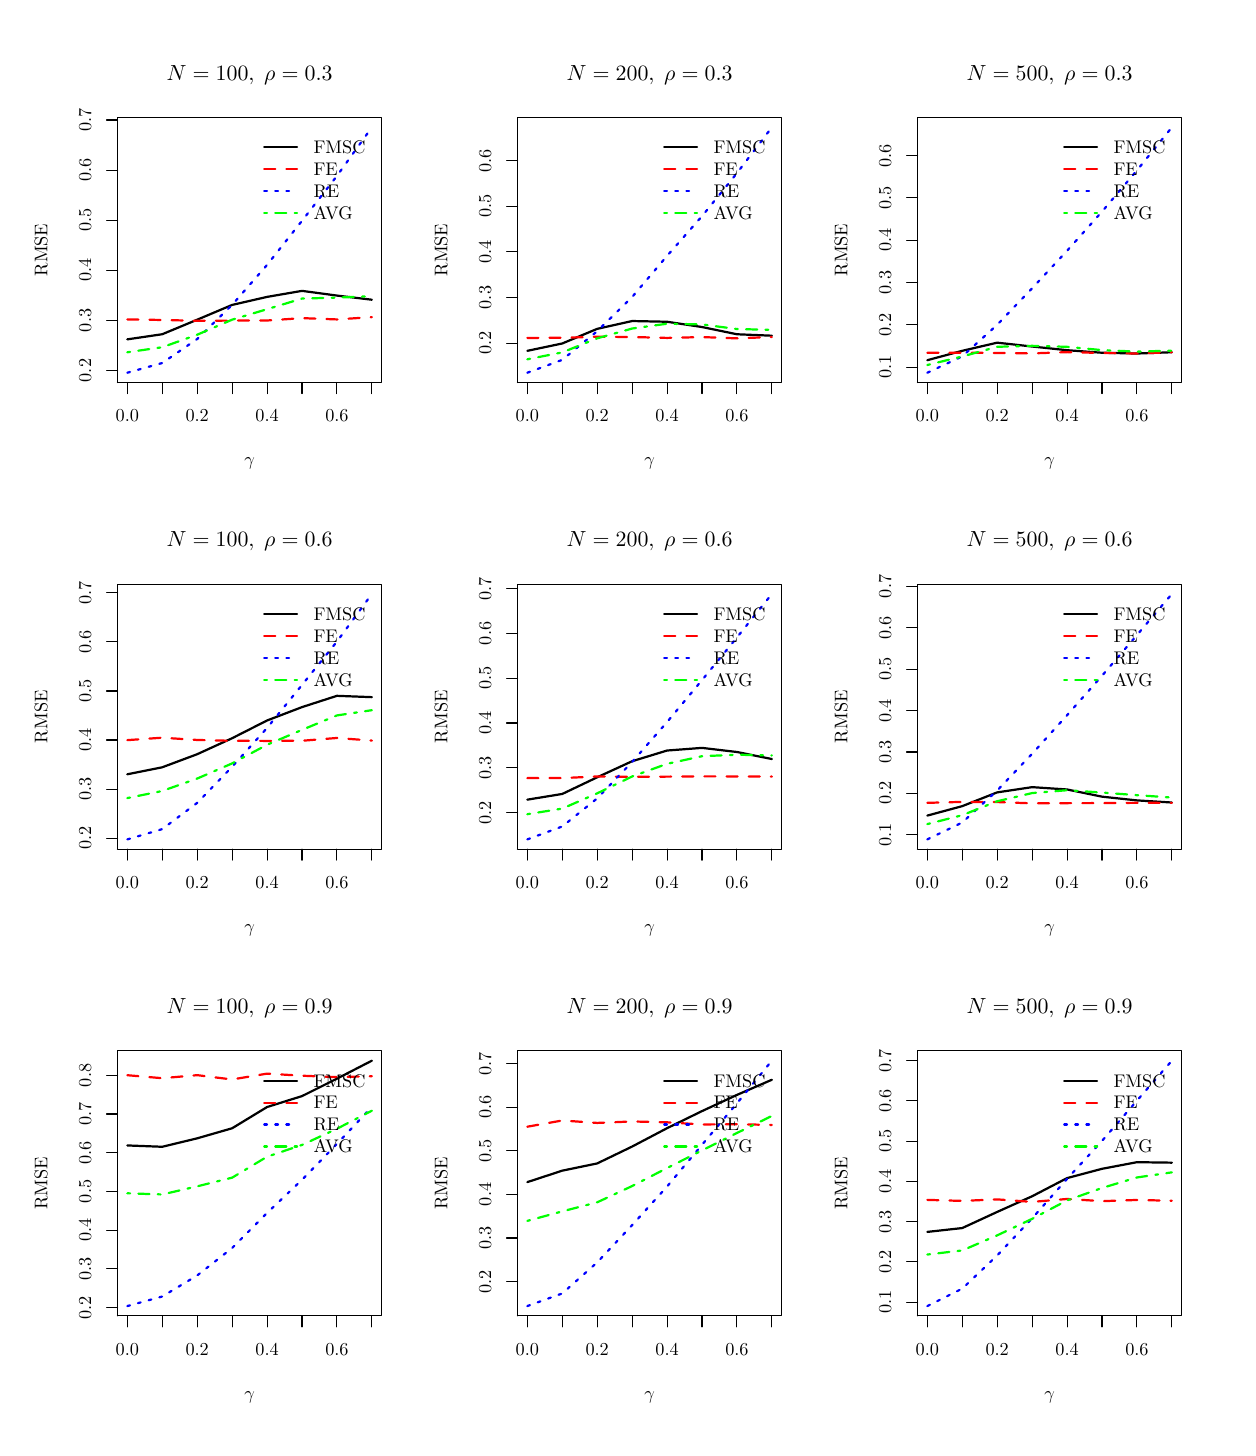
\begin{tikzpicture}[x=1pt,y=1pt]
\definecolor{fillColor}{RGB}{255,255,255}
\path[use as bounding box,fill=fillColor,fill opacity=0.00] (0,0) rectangle (433.62,505.89);
\begin{scope}
\path[clip] ( 32.47,377.65) rectangle (127.91,473.42);
\definecolor{drawColor}{RGB}{0,0,0}

\path[draw=drawColor,line width= 0.8pt,line join=round,line cap=round] ( 36.01,393.26) --
	( 48.63,395.11) --
	( 61.25,400.36) --
	( 73.88,405.70) --
	( 86.50,408.60) --
	( 99.13,410.78) --
	(111.75,409.08) --
	(124.37,407.58);
\end{scope}
\begin{scope}
\path[clip] (  0.00,  0.00) rectangle (433.62,505.89);
\definecolor{drawColor}{RGB}{0,0,0}

\path[draw=drawColor,line width= 0.4pt,line join=round,line cap=round] ( 36.01,377.65) -- (124.37,377.65);

\path[draw=drawColor,line width= 0.4pt,line join=round,line cap=round] ( 36.01,377.65) -- ( 36.01,373.69);

\path[draw=drawColor,line width= 0.4pt,line join=round,line cap=round] ( 48.63,377.65) -- ( 48.63,373.69);

\path[draw=drawColor,line width= 0.4pt,line join=round,line cap=round] ( 61.25,377.65) -- ( 61.25,373.69);

\path[draw=drawColor,line width= 0.4pt,line join=round,line cap=round] ( 73.88,377.65) -- ( 73.88,373.69);

\path[draw=drawColor,line width= 0.4pt,line join=round,line cap=round] ( 86.50,377.65) -- ( 86.50,373.69);

\path[draw=drawColor,line width= 0.4pt,line join=round,line cap=round] ( 99.13,377.65) -- ( 99.13,373.69);

\path[draw=drawColor,line width= 0.4pt,line join=round,line cap=round] (111.75,377.65) -- (111.75,373.69);

\path[draw=drawColor,line width= 0.4pt,line join=round,line cap=round] (124.37,377.65) -- (124.37,373.69);

\node[text=drawColor,anchor=base,inner sep=0pt, outer sep=0pt, scale=  0.66] at ( 36.01,363.40) {0.0};

\node[text=drawColor,anchor=base,inner sep=0pt, outer sep=0pt, scale=  0.66] at ( 61.25,363.40) {0.2};

\node[text=drawColor,anchor=base,inner sep=0pt, outer sep=0pt, scale=  0.66] at ( 86.50,363.40) {0.4};

\node[text=drawColor,anchor=base,inner sep=0pt, outer sep=0pt, scale=  0.66] at (111.75,363.40) {0.6};

\path[draw=drawColor,line width= 0.4pt,line join=round,line cap=round] ( 32.47,382.00) -- ( 32.47,472.53);

\path[draw=drawColor,line width= 0.4pt,line join=round,line cap=round] ( 32.47,382.00) -- ( 28.51,382.00);

\path[draw=drawColor,line width= 0.4pt,line join=round,line cap=round] ( 32.47,400.11) -- ( 28.51,400.11);

\path[draw=drawColor,line width= 0.4pt,line join=round,line cap=round] ( 32.47,418.21) -- ( 28.51,418.21);

\path[draw=drawColor,line width= 0.4pt,line join=round,line cap=round] ( 32.47,436.32) -- ( 28.51,436.32);

\path[draw=drawColor,line width= 0.4pt,line join=round,line cap=round] ( 32.47,454.43) -- ( 28.51,454.43);

\path[draw=drawColor,line width= 0.4pt,line join=round,line cap=round] ( 32.47,472.53) -- ( 28.51,472.53);

\node[text=drawColor,rotate= 90.00,anchor=base,inner sep=0pt, outer sep=0pt, scale=  0.66] at ( 22.97,382.00) {0.2};

\node[text=drawColor,rotate= 90.00,anchor=base,inner sep=0pt, outer sep=0pt, scale=  0.66] at ( 22.97,400.11) {0.3};

\node[text=drawColor,rotate= 90.00,anchor=base,inner sep=0pt, outer sep=0pt, scale=  0.66] at ( 22.97,418.21) {0.4};

\node[text=drawColor,rotate= 90.00,anchor=base,inner sep=0pt, outer sep=0pt, scale=  0.66] at ( 22.97,436.32) {0.5};

\node[text=drawColor,rotate= 90.00,anchor=base,inner sep=0pt, outer sep=0pt, scale=  0.66] at ( 22.97,454.43) {0.6};

\node[text=drawColor,rotate= 90.00,anchor=base,inner sep=0pt, outer sep=0pt, scale=  0.66] at ( 22.97,472.53) {0.7};

\path[draw=drawColor,line width= 0.4pt,line join=round,line cap=round] ( 32.47,377.65) --
	(127.91,377.65) --
	(127.91,473.42) --
	( 32.47,473.42) --
	( 32.47,377.65);
\end{scope}
\begin{scope}
\path[clip] (  0.00,337.26) rectangle (144.54,505.89);
\definecolor{drawColor}{RGB}{0,0,0}

\node[text=drawColor,anchor=base,inner sep=0pt, outer sep=0pt, scale=  0.79] at ( 80.19,486.92) {\bfseries $N=100, \;\rho=0.3$};

\node[text=drawColor,anchor=base,inner sep=0pt, outer sep=0pt, scale=  0.66] at ( 80.19,347.56) {$\gamma$};

\node[text=drawColor,rotate= 90.00,anchor=base,inner sep=0pt, outer sep=0pt, scale=  0.66] at (  7.13,425.53) {RMSE};
\end{scope}
\begin{scope}
\path[clip] ( 32.47,377.65) rectangle (127.91,473.42);
\definecolor{drawColor}{RGB}{255,0,0}

\path[draw=drawColor,line width= 0.8pt,dash pattern=on 4pt off 4pt ,line join=round,line cap=round] ( 36.01,400.47) --
	( 48.63,400.26) --
	( 61.25,399.97) --
	( 73.88,400.04) --
	( 86.50,400.07) --
	( 99.13,400.93) --
	(111.75,400.46) --
	(124.37,401.29);
\definecolor{drawColor}{RGB}{0,0,255}

\path[draw=drawColor,line width= 0.8pt,dash pattern=on 1pt off 3pt ,line join=round,line cap=round] ( 36.01,381.20) --
	( 48.63,384.71) --
	( 61.25,393.38) --
	( 73.88,405.72) --
	( 86.50,420.15) --
	( 99.13,436.10) --
	(111.75,452.31) --
	(124.37,469.87);
\definecolor{drawColor}{RGB}{0,255,0}

\path[draw=drawColor,line width= 0.8pt,dash pattern=on 1pt off 3pt on 4pt off 3pt ,line join=round,line cap=round] ( 36.01,388.59) --
	( 48.63,390.41) --
	( 61.25,394.93) --
	( 73.88,400.37) --
	( 86.50,404.15) --
	( 99.13,407.99) --
	(111.75,408.35) --
	(124.37,408.84);
\definecolor{drawColor}{RGB}{0,0,0}

\path[draw=drawColor,line width= 0.8pt,line join=round,line cap=round] ( 85.47,462.63) -- ( 97.35,462.63);
\definecolor{drawColor}{RGB}{255,0,0}

\path[draw=drawColor,line width= 0.8pt,dash pattern=on 4pt off 4pt ,line join=round,line cap=round] ( 85.47,454.71) -- ( 97.35,454.71);
\definecolor{drawColor}{RGB}{0,0,255}

\path[draw=drawColor,line width= 0.8pt,dash pattern=on 1pt off 3pt ,line join=round,line cap=round] ( 85.47,446.79) -- ( 97.35,446.79);
\definecolor{drawColor}{RGB}{0,255,0}

\path[draw=drawColor,line width= 0.8pt,dash pattern=on 1pt off 3pt on 4pt off 3pt ,line join=round,line cap=round] ( 85.47,438.87) -- ( 97.35,438.87);
\definecolor{drawColor}{RGB}{0,0,0}

\node[text=drawColor,anchor=base west,inner sep=0pt, outer sep=0pt, scale=  0.66] at (103.29,460.35) {FMSC};

\node[text=drawColor,anchor=base west,inner sep=0pt, outer sep=0pt, scale=  0.66] at (103.29,452.43) {FE};

\node[text=drawColor,anchor=base west,inner sep=0pt, outer sep=0pt, scale=  0.66] at (103.29,444.51) {RE};

\node[text=drawColor,anchor=base west,inner sep=0pt, outer sep=0pt, scale=  0.66] at (103.29,436.59) {AVG};
\end{scope}
\begin{scope}
\path[clip] (177.01,377.65) rectangle (272.45,473.42);
\definecolor{drawColor}{RGB}{0,0,0}

\path[draw=drawColor,line width= 0.8pt,line join=round,line cap=round] (180.55,389.11) --
	(193.17,391.77) --
	(205.79,397.05) --
	(218.42,399.88) --
	(231.04,399.62) --
	(243.67,397.71) --
	(256.29,395.10) --
	(268.91,394.58);
\end{scope}
\begin{scope}
\path[clip] (  0.00,  0.00) rectangle (433.62,505.89);
\definecolor{drawColor}{RGB}{0,0,0}

\path[draw=drawColor,line width= 0.4pt,line join=round,line cap=round] (180.55,377.65) -- (268.91,377.65);

\path[draw=drawColor,line width= 0.4pt,line join=round,line cap=round] (180.55,377.65) -- (180.55,373.69);

\path[draw=drawColor,line width= 0.4pt,line join=round,line cap=round] (193.17,377.65) -- (193.17,373.69);

\path[draw=drawColor,line width= 0.4pt,line join=round,line cap=round] (205.79,377.65) -- (205.79,373.69);

\path[draw=drawColor,line width= 0.4pt,line join=round,line cap=round] (218.42,377.65) -- (218.42,373.69);

\path[draw=drawColor,line width= 0.4pt,line join=round,line cap=round] (231.04,377.65) -- (231.04,373.69);

\path[draw=drawColor,line width= 0.4pt,line join=round,line cap=round] (243.67,377.65) -- (243.67,373.69);

\path[draw=drawColor,line width= 0.4pt,line join=round,line cap=round] (256.29,377.65) -- (256.29,373.69);

\path[draw=drawColor,line width= 0.4pt,line join=round,line cap=round] (268.91,377.65) -- (268.91,373.69);

\node[text=drawColor,anchor=base,inner sep=0pt, outer sep=0pt, scale=  0.66] at (180.55,363.40) {0.0};

\node[text=drawColor,anchor=base,inner sep=0pt, outer sep=0pt, scale=  0.66] at (205.79,363.40) {0.2};

\node[text=drawColor,anchor=base,inner sep=0pt, outer sep=0pt, scale=  0.66] at (231.04,363.40) {0.4};

\node[text=drawColor,anchor=base,inner sep=0pt, outer sep=0pt, scale=  0.66] at (256.29,363.40) {0.6};

\path[draw=drawColor,line width= 0.4pt,line join=round,line cap=round] (177.01,391.89) -- (177.01,457.84);

\path[draw=drawColor,line width= 0.4pt,line join=round,line cap=round] (177.01,391.89) -- (173.05,391.89);

\path[draw=drawColor,line width= 0.4pt,line join=round,line cap=round] (177.01,408.38) -- (173.05,408.38);

\path[draw=drawColor,line width= 0.4pt,line join=round,line cap=round] (177.01,424.86) -- (173.05,424.86);

\path[draw=drawColor,line width= 0.4pt,line join=round,line cap=round] (177.01,441.35) -- (173.05,441.35);

\path[draw=drawColor,line width= 0.4pt,line join=round,line cap=round] (177.01,457.84) -- (173.05,457.84);

\node[text=drawColor,rotate= 90.00,anchor=base,inner sep=0pt, outer sep=0pt, scale=  0.66] at (167.51,391.89) {0.2};

\node[text=drawColor,rotate= 90.00,anchor=base,inner sep=0pt, outer sep=0pt, scale=  0.66] at (167.51,408.38) {0.3};

\node[text=drawColor,rotate= 90.00,anchor=base,inner sep=0pt, outer sep=0pt, scale=  0.66] at (167.51,424.86) {0.4};

\node[text=drawColor,rotate= 90.00,anchor=base,inner sep=0pt, outer sep=0pt, scale=  0.66] at (167.51,441.35) {0.5};

\node[text=drawColor,rotate= 90.00,anchor=base,inner sep=0pt, outer sep=0pt, scale=  0.66] at (167.51,457.84) {0.6};

\path[draw=drawColor,line width= 0.4pt,line join=round,line cap=round] (177.01,377.65) --
	(272.45,377.65) --
	(272.45,473.42) --
	(177.01,473.42) --
	(177.01,377.65);
\end{scope}
\begin{scope}
\path[clip] (144.54,337.26) rectangle (289.08,505.89);
\definecolor{drawColor}{RGB}{0,0,0}

\node[text=drawColor,anchor=base,inner sep=0pt, outer sep=0pt, scale=  0.79] at (224.73,486.92) {\bfseries $N=200, \;\rho=0.3$};

\node[text=drawColor,anchor=base,inner sep=0pt, outer sep=0pt, scale=  0.66] at (224.73,347.56) {$\gamma$};

\node[text=drawColor,rotate= 90.00,anchor=base,inner sep=0pt, outer sep=0pt, scale=  0.66] at (151.67,425.53) {RMSE};
\end{scope}
\begin{scope}
\path[clip] (177.01,377.65) rectangle (272.45,473.42);
\definecolor{drawColor}{RGB}{255,0,0}

\path[draw=drawColor,line width= 0.8pt,dash pattern=on 4pt off 4pt ,line join=round,line cap=round] (180.55,393.76) --
	(193.17,393.83) --
	(205.79,394.20) --
	(218.42,394.11) --
	(231.04,393.78) --
	(243.67,394.08) --
	(256.29,393.62) --
	(268.91,394.10);
\definecolor{drawColor}{RGB}{0,0,255}

\path[draw=drawColor,line width= 0.8pt,dash pattern=on 1pt off 3pt ,line join=round,line cap=round] (180.55,381.20) --
	(193.17,385.85) --
	(205.79,396.20) --
	(218.42,408.56) --
	(231.04,423.41) --
	(243.67,437.77) --
	(256.29,453.32) --
	(268.91,469.87);
\definecolor{drawColor}{RGB}{0,255,0}

\path[draw=drawColor,line width= 0.8pt,dash pattern=on 1pt off 3pt on 4pt off 3pt ,line join=round,line cap=round] (180.55,386.05) --
	(193.17,388.54) --
	(205.79,393.63) --
	(218.42,397.17) --
	(231.04,398.91) --
	(243.67,398.66) --
	(256.29,396.98) --
	(268.91,396.70);
\definecolor{drawColor}{RGB}{0,0,0}

\path[draw=drawColor,line width= 0.8pt,line join=round,line cap=round] (230.01,462.63) -- (241.89,462.63);
\definecolor{drawColor}{RGB}{255,0,0}

\path[draw=drawColor,line width= 0.8pt,dash pattern=on 4pt off 4pt ,line join=round,line cap=round] (230.01,454.71) -- (241.89,454.71);
\definecolor{drawColor}{RGB}{0,0,255}

\path[draw=drawColor,line width= 0.8pt,dash pattern=on 1pt off 3pt ,line join=round,line cap=round] (230.01,446.79) -- (241.89,446.79);
\definecolor{drawColor}{RGB}{0,255,0}

\path[draw=drawColor,line width= 0.8pt,dash pattern=on 1pt off 3pt on 4pt off 3pt ,line join=round,line cap=round] (230.01,438.87) -- (241.89,438.87);
\definecolor{drawColor}{RGB}{0,0,0}

\node[text=drawColor,anchor=base west,inner sep=0pt, outer sep=0pt, scale=  0.66] at (247.83,460.35) {FMSC};

\node[text=drawColor,anchor=base west,inner sep=0pt, outer sep=0pt, scale=  0.66] at (247.83,452.43) {FE};

\node[text=drawColor,anchor=base west,inner sep=0pt, outer sep=0pt, scale=  0.66] at (247.83,444.51) {RE};

\node[text=drawColor,anchor=base west,inner sep=0pt, outer sep=0pt, scale=  0.66] at (247.83,436.59) {AVG};
\end{scope}
\begin{scope}
\path[clip] (321.55,377.65) rectangle (416.99,473.42);
\definecolor{drawColor}{RGB}{0,0,0}

\path[draw=drawColor,line width= 0.8pt,line join=round,line cap=round] (325.09,385.73) --
	(337.71,389.12) --
	(350.33,392.06) --
	(362.96,390.67) --
	(375.58,389.34) --
	(388.21,388.42) --
	(400.83,388.14) --
	(413.45,388.60);
\end{scope}
\begin{scope}
\path[clip] (  0.00,  0.00) rectangle (433.62,505.89);
\definecolor{drawColor}{RGB}{0,0,0}

\path[draw=drawColor,line width= 0.4pt,line join=round,line cap=round] (325.09,377.65) -- (413.45,377.65);

\path[draw=drawColor,line width= 0.4pt,line join=round,line cap=round] (325.09,377.65) -- (325.09,373.69);

\path[draw=drawColor,line width= 0.4pt,line join=round,line cap=round] (337.71,377.65) -- (337.71,373.69);

\path[draw=drawColor,line width= 0.4pt,line join=round,line cap=round] (350.33,377.65) -- (350.33,373.69);

\path[draw=drawColor,line width= 0.4pt,line join=round,line cap=round] (362.96,377.65) -- (362.96,373.69);

\path[draw=drawColor,line width= 0.4pt,line join=round,line cap=round] (375.58,377.65) -- (375.58,373.69);

\path[draw=drawColor,line width= 0.4pt,line join=round,line cap=round] (388.21,377.65) -- (388.21,373.69);

\path[draw=drawColor,line width= 0.4pt,line join=round,line cap=round] (400.83,377.65) -- (400.83,373.69);

\path[draw=drawColor,line width= 0.4pt,line join=round,line cap=round] (413.45,377.65) -- (413.45,373.69);

\node[text=drawColor,anchor=base,inner sep=0pt, outer sep=0pt, scale=  0.66] at (325.09,363.40) {0.0};

\node[text=drawColor,anchor=base,inner sep=0pt, outer sep=0pt, scale=  0.66] at (350.33,363.40) {0.2};

\node[text=drawColor,anchor=base,inner sep=0pt, outer sep=0pt, scale=  0.66] at (375.58,363.40) {0.4};

\node[text=drawColor,anchor=base,inner sep=0pt, outer sep=0pt, scale=  0.66] at (400.83,363.40) {0.6};

\path[draw=drawColor,line width= 0.4pt,line join=round,line cap=round] (321.55,383.23) -- (321.55,459.65);

\path[draw=drawColor,line width= 0.4pt,line join=round,line cap=round] (321.55,383.23) -- (317.59,383.23);

\path[draw=drawColor,line width= 0.4pt,line join=round,line cap=round] (321.55,398.51) -- (317.59,398.51);

\path[draw=drawColor,line width= 0.4pt,line join=round,line cap=round] (321.55,413.80) -- (317.59,413.80);

\path[draw=drawColor,line width= 0.4pt,line join=round,line cap=round] (321.55,429.08) -- (317.59,429.08);

\path[draw=drawColor,line width= 0.4pt,line join=round,line cap=round] (321.55,444.37) -- (317.59,444.37);

\path[draw=drawColor,line width= 0.4pt,line join=round,line cap=round] (321.55,459.65) -- (317.59,459.65);

\node[text=drawColor,rotate= 90.00,anchor=base,inner sep=0pt, outer sep=0pt, scale=  0.66] at (312.05,383.23) {0.1};

\node[text=drawColor,rotate= 90.00,anchor=base,inner sep=0pt, outer sep=0pt, scale=  0.66] at (312.05,398.51) {0.2};

\node[text=drawColor,rotate= 90.00,anchor=base,inner sep=0pt, outer sep=0pt, scale=  0.66] at (312.05,413.80) {0.3};

\node[text=drawColor,rotate= 90.00,anchor=base,inner sep=0pt, outer sep=0pt, scale=  0.66] at (312.05,429.08) {0.4};

\node[text=drawColor,rotate= 90.00,anchor=base,inner sep=0pt, outer sep=0pt, scale=  0.66] at (312.05,444.37) {0.5};

\node[text=drawColor,rotate= 90.00,anchor=base,inner sep=0pt, outer sep=0pt, scale=  0.66] at (312.05,459.65) {0.6};

\path[draw=drawColor,line width= 0.4pt,line join=round,line cap=round] (321.55,377.65) --
	(416.99,377.65) --
	(416.99,473.42) --
	(321.55,473.42) --
	(321.55,377.65);
\end{scope}
\begin{scope}
\path[clip] (289.08,337.26) rectangle (433.62,505.89);
\definecolor{drawColor}{RGB}{0,0,0}

\node[text=drawColor,anchor=base,inner sep=0pt, outer sep=0pt, scale=  0.79] at (369.27,486.92) {\bfseries $N=500, \;\rho=0.3$};

\node[text=drawColor,anchor=base,inner sep=0pt, outer sep=0pt, scale=  0.66] at (369.27,347.56) {$\gamma$};

\node[text=drawColor,rotate= 90.00,anchor=base,inner sep=0pt, outer sep=0pt, scale=  0.66] at (296.21,425.53) {RMSE};
\end{scope}
\begin{scope}
\path[clip] (321.55,377.65) rectangle (416.99,473.42);
\definecolor{drawColor}{RGB}{255,0,0}

\path[draw=drawColor,line width= 0.8pt,dash pattern=on 4pt off 4pt ,line join=round,line cap=round] (325.09,388.41) --
	(337.71,388.44) --
	(350.33,388.35) --
	(362.96,388.18) --
	(375.58,388.64) --
	(388.21,388.35) --
	(400.83,388.14) --
	(413.45,388.60);
\definecolor{drawColor}{RGB}{0,0,255}

\path[draw=drawColor,line width= 0.8pt,dash pattern=on 1pt off 3pt ,line join=round,line cap=round] (325.09,381.20) --
	(337.71,387.10) --
	(350.33,398.52) --
	(362.96,411.72) --
	(375.58,425.26) --
	(388.21,439.42) --
	(400.83,454.32) --
	(413.45,469.87);
\definecolor{drawColor}{RGB}{0,255,0}

\path[draw=drawColor,line width= 0.8pt,dash pattern=on 1pt off 3pt on 4pt off 3pt ,line join=round,line cap=round] (325.09,383.99) --
	(337.71,387.07) --
	(350.33,390.57) --
	(362.96,390.92) --
	(375.58,390.56) --
	(388.21,389.37) --
	(400.83,388.83) --
	(413.45,389.18);
\definecolor{drawColor}{RGB}{0,0,0}

\path[draw=drawColor,line width= 0.8pt,line join=round,line cap=round] (374.55,462.63) -- (386.43,462.63);
\definecolor{drawColor}{RGB}{255,0,0}

\path[draw=drawColor,line width= 0.8pt,dash pattern=on 4pt off 4pt ,line join=round,line cap=round] (374.55,454.71) -- (386.43,454.71);
\definecolor{drawColor}{RGB}{0,0,255}

\path[draw=drawColor,line width= 0.8pt,dash pattern=on 1pt off 3pt ,line join=round,line cap=round] (374.55,446.79) -- (386.43,446.79);
\definecolor{drawColor}{RGB}{0,255,0}

\path[draw=drawColor,line width= 0.8pt,dash pattern=on 1pt off 3pt on 4pt off 3pt ,line join=round,line cap=round] (374.55,438.87) -- (386.43,438.87);
\definecolor{drawColor}{RGB}{0,0,0}

\node[text=drawColor,anchor=base west,inner sep=0pt, outer sep=0pt, scale=  0.66] at (392.37,460.35) {FMSC};

\node[text=drawColor,anchor=base west,inner sep=0pt, outer sep=0pt, scale=  0.66] at (392.37,452.43) {FE};

\node[text=drawColor,anchor=base west,inner sep=0pt, outer sep=0pt, scale=  0.66] at (392.37,444.51) {RE};

\node[text=drawColor,anchor=base west,inner sep=0pt, outer sep=0pt, scale=  0.66] at (392.37,436.59) {AVG};
\end{scope}
\begin{scope}
\path[clip] ( 32.47,209.02) rectangle (127.91,304.79);
\definecolor{drawColor}{RGB}{0,0,0}

\path[draw=drawColor,line width= 0.8pt,line join=round,line cap=round] ( 36.01,236.10) --
	( 48.63,238.63) --
	( 61.25,243.35) --
	( 73.88,249.13) --
	( 86.50,255.54) --
	( 99.13,260.37) --
	(111.75,264.45) --
	(124.37,263.97);
\end{scope}
\begin{scope}
\path[clip] (  0.00,  0.00) rectangle (433.62,505.89);
\definecolor{drawColor}{RGB}{0,0,0}

\path[draw=drawColor,line width= 0.4pt,line join=round,line cap=round] ( 36.01,209.02) -- (124.37,209.02);

\path[draw=drawColor,line width= 0.4pt,line join=round,line cap=round] ( 36.01,209.02) -- ( 36.01,205.06);

\path[draw=drawColor,line width= 0.4pt,line join=round,line cap=round] ( 48.63,209.02) -- ( 48.63,205.06);

\path[draw=drawColor,line width= 0.4pt,line join=round,line cap=round] ( 61.25,209.02) -- ( 61.25,205.06);

\path[draw=drawColor,line width= 0.4pt,line join=round,line cap=round] ( 73.88,209.02) -- ( 73.88,205.06);

\path[draw=drawColor,line width= 0.4pt,line join=round,line cap=round] ( 86.50,209.02) -- ( 86.50,205.06);

\path[draw=drawColor,line width= 0.4pt,line join=round,line cap=round] ( 99.13,209.02) -- ( 99.13,205.06);

\path[draw=drawColor,line width= 0.4pt,line join=round,line cap=round] (111.75,209.02) -- (111.75,205.06);

\path[draw=drawColor,line width= 0.4pt,line join=round,line cap=round] (124.37,209.02) -- (124.37,205.06);

\node[text=drawColor,anchor=base,inner sep=0pt, outer sep=0pt, scale=  0.66] at ( 36.01,194.77) {0.0};

\node[text=drawColor,anchor=base,inner sep=0pt, outer sep=0pt, scale=  0.66] at ( 61.25,194.77) {0.2};

\node[text=drawColor,anchor=base,inner sep=0pt, outer sep=0pt, scale=  0.66] at ( 86.50,194.77) {0.4};

\node[text=drawColor,anchor=base,inner sep=0pt, outer sep=0pt, scale=  0.66] at (111.75,194.77) {0.6};

\path[draw=drawColor,line width= 0.4pt,line join=round,line cap=round] ( 32.47,213.01) -- ( 32.47,301.66);

\path[draw=drawColor,line width= 0.4pt,line join=round,line cap=round] ( 32.47,213.01) -- ( 28.51,213.01);

\path[draw=drawColor,line width= 0.4pt,line join=round,line cap=round] ( 32.47,230.74) -- ( 28.51,230.74);

\path[draw=drawColor,line width= 0.4pt,line join=round,line cap=round] ( 32.47,248.47) -- ( 28.51,248.47);

\path[draw=drawColor,line width= 0.4pt,line join=round,line cap=round] ( 32.47,266.20) -- ( 28.51,266.20);

\path[draw=drawColor,line width= 0.4pt,line join=round,line cap=round] ( 32.47,283.93) -- ( 28.51,283.93);

\path[draw=drawColor,line width= 0.4pt,line join=round,line cap=round] ( 32.47,301.66) -- ( 28.51,301.66);

\node[text=drawColor,rotate= 90.00,anchor=base,inner sep=0pt, outer sep=0pt, scale=  0.66] at ( 22.97,213.01) {0.2};

\node[text=drawColor,rotate= 90.00,anchor=base,inner sep=0pt, outer sep=0pt, scale=  0.66] at ( 22.97,230.74) {0.3};

\node[text=drawColor,rotate= 90.00,anchor=base,inner sep=0pt, outer sep=0pt, scale=  0.66] at ( 22.97,248.47) {0.4};

\node[text=drawColor,rotate= 90.00,anchor=base,inner sep=0pt, outer sep=0pt, scale=  0.66] at ( 22.97,266.20) {0.5};

\node[text=drawColor,rotate= 90.00,anchor=base,inner sep=0pt, outer sep=0pt, scale=  0.66] at ( 22.97,283.93) {0.6};

\node[text=drawColor,rotate= 90.00,anchor=base,inner sep=0pt, outer sep=0pt, scale=  0.66] at ( 22.97,301.66) {0.7};

\path[draw=drawColor,line width= 0.4pt,line join=round,line cap=round] ( 32.47,209.02) --
	(127.91,209.02) --
	(127.91,304.79) --
	( 32.47,304.79) --
	( 32.47,209.02);
\end{scope}
\begin{scope}
\path[clip] (  0.00,168.63) rectangle (144.54,337.26);
\definecolor{drawColor}{RGB}{0,0,0}

\node[text=drawColor,anchor=base,inner sep=0pt, outer sep=0pt, scale=  0.79] at ( 80.19,318.29) {\bfseries $N=100, \;\rho=0.6$};

\node[text=drawColor,anchor=base,inner sep=0pt, outer sep=0pt, scale=  0.66] at ( 80.19,178.93) {$\gamma$};

\node[text=drawColor,rotate= 90.00,anchor=base,inner sep=0pt, outer sep=0pt, scale=  0.66] at (  7.13,256.90) {RMSE};
\end{scope}
\begin{scope}
\path[clip] ( 32.47,209.02) rectangle (127.91,304.79);
\definecolor{drawColor}{RGB}{255,0,0}

\path[draw=drawColor,line width= 0.8pt,dash pattern=on 4pt off 4pt ,line join=round,line cap=round] ( 36.01,248.44) --
	( 48.63,249.32) --
	( 61.25,248.50) --
	( 73.88,248.20) --
	( 86.50,248.16) --
	( 99.13,248.21) --
	(111.75,249.22) --
	(124.37,248.27);
\definecolor{drawColor}{RGB}{0,0,255}

\path[draw=drawColor,line width= 0.8pt,dash pattern=on 1pt off 3pt ,line join=round,line cap=round] ( 36.01,212.57) --
	( 48.63,216.29) --
	( 61.25,225.77) --
	( 73.88,238.80) --
	( 86.50,252.84) --
	( 99.13,268.38) --
	(111.75,284.05) --
	(124.37,301.24);
\definecolor{drawColor}{RGB}{0,255,0}

\path[draw=drawColor,line width= 0.8pt,dash pattern=on 1pt off 3pt on 4pt off 3pt ,line join=round,line cap=round] ( 36.01,227.49) --
	( 48.63,230.07) --
	( 61.25,234.55) --
	( 73.88,240.03) --
	( 86.50,246.77) --
	( 99.13,252.15) --
	(111.75,257.37) --
	(124.37,259.26);
\definecolor{drawColor}{RGB}{0,0,0}

\path[draw=drawColor,line width= 0.8pt,line join=round,line cap=round] ( 85.47,294.00) -- ( 97.35,294.00);
\definecolor{drawColor}{RGB}{255,0,0}

\path[draw=drawColor,line width= 0.8pt,dash pattern=on 4pt off 4pt ,line join=round,line cap=round] ( 85.47,286.08) -- ( 97.35,286.08);
\definecolor{drawColor}{RGB}{0,0,255}

\path[draw=drawColor,line width= 0.8pt,dash pattern=on 1pt off 3pt ,line join=round,line cap=round] ( 85.47,278.16) -- ( 97.35,278.16);
\definecolor{drawColor}{RGB}{0,255,0}

\path[draw=drawColor,line width= 0.8pt,dash pattern=on 1pt off 3pt on 4pt off 3pt ,line join=round,line cap=round] ( 85.47,270.24) -- ( 97.35,270.24);
\definecolor{drawColor}{RGB}{0,0,0}

\node[text=drawColor,anchor=base west,inner sep=0pt, outer sep=0pt, scale=  0.66] at (103.29,291.72) {FMSC};

\node[text=drawColor,anchor=base west,inner sep=0pt, outer sep=0pt, scale=  0.66] at (103.29,283.80) {FE};

\node[text=drawColor,anchor=base west,inner sep=0pt, outer sep=0pt, scale=  0.66] at (103.29,275.88) {RE};

\node[text=drawColor,anchor=base west,inner sep=0pt, outer sep=0pt, scale=  0.66] at (103.29,267.96) {AVG};
\end{scope}
\begin{scope}
\path[clip] (177.01,209.02) rectangle (272.45,304.79);
\definecolor{drawColor}{RGB}{0,0,0}

\path[draw=drawColor,line width= 0.8pt,line join=round,line cap=round] (180.55,226.93) --
	(193.17,228.99) --
	(205.79,235.01) --
	(218.42,240.82) --
	(231.04,244.68) --
	(243.67,245.64) --
	(256.29,244.15) --
	(268.91,241.61);
\end{scope}
\begin{scope}
\path[clip] (  0.00,  0.00) rectangle (433.62,505.89);
\definecolor{drawColor}{RGB}{0,0,0}

\path[draw=drawColor,line width= 0.4pt,line join=round,line cap=round] (180.55,209.02) -- (268.91,209.02);

\path[draw=drawColor,line width= 0.4pt,line join=round,line cap=round] (180.55,209.02) -- (180.55,205.06);

\path[draw=drawColor,line width= 0.4pt,line join=round,line cap=round] (193.17,209.02) -- (193.17,205.06);

\path[draw=drawColor,line width= 0.4pt,line join=round,line cap=round] (205.79,209.02) -- (205.79,205.06);

\path[draw=drawColor,line width= 0.4pt,line join=round,line cap=round] (218.42,209.02) -- (218.42,205.06);

\path[draw=drawColor,line width= 0.4pt,line join=round,line cap=round] (231.04,209.02) -- (231.04,205.06);

\path[draw=drawColor,line width= 0.4pt,line join=round,line cap=round] (243.67,209.02) -- (243.67,205.06);

\path[draw=drawColor,line width= 0.4pt,line join=round,line cap=round] (256.29,209.02) -- (256.29,205.06);

\path[draw=drawColor,line width= 0.4pt,line join=round,line cap=round] (268.91,209.02) -- (268.91,205.06);

\node[text=drawColor,anchor=base,inner sep=0pt, outer sep=0pt, scale=  0.66] at (180.55,194.77) {0.0};

\node[text=drawColor,anchor=base,inner sep=0pt, outer sep=0pt, scale=  0.66] at (205.79,194.77) {0.2};

\node[text=drawColor,anchor=base,inner sep=0pt, outer sep=0pt, scale=  0.66] at (231.04,194.77) {0.4};

\node[text=drawColor,anchor=base,inner sep=0pt, outer sep=0pt, scale=  0.66] at (256.29,194.77) {0.6};

\path[draw=drawColor,line width= 0.4pt,line join=round,line cap=round] (177.01,222.23) -- (177.01,303.21);

\path[draw=drawColor,line width= 0.4pt,line join=round,line cap=round] (177.01,222.23) -- (173.05,222.23);

\path[draw=drawColor,line width= 0.4pt,line join=round,line cap=round] (177.01,238.42) -- (173.05,238.42);

\path[draw=drawColor,line width= 0.4pt,line join=round,line cap=round] (177.01,254.62) -- (173.05,254.62);

\path[draw=drawColor,line width= 0.4pt,line join=round,line cap=round] (177.01,270.82) -- (173.05,270.82);

\path[draw=drawColor,line width= 0.4pt,line join=round,line cap=round] (177.01,287.02) -- (173.05,287.02);

\path[draw=drawColor,line width= 0.4pt,line join=round,line cap=round] (177.01,303.21) -- (173.05,303.21);

\node[text=drawColor,rotate= 90.00,anchor=base,inner sep=0pt, outer sep=0pt, scale=  0.66] at (167.51,222.23) {0.2};

\node[text=drawColor,rotate= 90.00,anchor=base,inner sep=0pt, outer sep=0pt, scale=  0.66] at (167.51,238.42) {0.3};

\node[text=drawColor,rotate= 90.00,anchor=base,inner sep=0pt, outer sep=0pt, scale=  0.66] at (167.51,254.62) {0.4};

\node[text=drawColor,rotate= 90.00,anchor=base,inner sep=0pt, outer sep=0pt, scale=  0.66] at (167.51,270.82) {0.5};

\node[text=drawColor,rotate= 90.00,anchor=base,inner sep=0pt, outer sep=0pt, scale=  0.66] at (167.51,287.02) {0.6};

\node[text=drawColor,rotate= 90.00,anchor=base,inner sep=0pt, outer sep=0pt, scale=  0.66] at (167.51,303.21) {0.7};

\path[draw=drawColor,line width= 0.4pt,line join=round,line cap=round] (177.01,209.02) --
	(272.45,209.02) --
	(272.45,304.79) --
	(177.01,304.79) --
	(177.01,209.02);
\end{scope}
\begin{scope}
\path[clip] (144.54,168.63) rectangle (289.08,337.26);
\definecolor{drawColor}{RGB}{0,0,0}

\node[text=drawColor,anchor=base,inner sep=0pt, outer sep=0pt, scale=  0.79] at (224.73,318.29) {\bfseries $N=200, \;\rho=0.6$};

\node[text=drawColor,anchor=base,inner sep=0pt, outer sep=0pt, scale=  0.66] at (224.73,178.93) {$\gamma$};

\node[text=drawColor,rotate= 90.00,anchor=base,inner sep=0pt, outer sep=0pt, scale=  0.66] at (151.67,256.90) {RMSE};
\end{scope}
\begin{scope}
\path[clip] (177.01,209.02) rectangle (272.45,304.79);
\definecolor{drawColor}{RGB}{255,0,0}

\path[draw=drawColor,line width= 0.8pt,dash pattern=on 4pt off 4pt ,line join=round,line cap=round] (180.55,234.73) --
	(193.17,234.72) --
	(205.79,235.31) --
	(218.42,235.18) --
	(231.04,235.25) --
	(243.67,235.35) --
	(256.29,235.32) --
	(268.91,235.28);
\definecolor{drawColor}{RGB}{0,0,255}

\path[draw=drawColor,line width= 0.8pt,dash pattern=on 1pt off 3pt ,line join=round,line cap=round] (180.55,212.57) --
	(193.17,217.24) --
	(205.79,227.39) --
	(218.42,240.56) --
	(231.04,254.96) --
	(243.67,270.13) --
	(256.29,285.55) --
	(268.91,301.24);
\definecolor{drawColor}{RGB}{0,255,0}

\path[draw=drawColor,line width= 0.8pt,dash pattern=on 1pt off 3pt on 4pt off 3pt ,line join=round,line cap=round] (180.55,221.67) --
	(193.17,223.70) --
	(205.79,229.21) --
	(218.42,235.31) --
	(231.04,239.88) --
	(243.67,242.63) --
	(256.29,243.17) --
	(268.91,242.90);
\definecolor{drawColor}{RGB}{0,0,0}

\path[draw=drawColor,line width= 0.8pt,line join=round,line cap=round] (230.01,294.00) -- (241.89,294.00);
\definecolor{drawColor}{RGB}{255,0,0}

\path[draw=drawColor,line width= 0.8pt,dash pattern=on 4pt off 4pt ,line join=round,line cap=round] (230.01,286.08) -- (241.89,286.08);
\definecolor{drawColor}{RGB}{0,0,255}

\path[draw=drawColor,line width= 0.8pt,dash pattern=on 1pt off 3pt ,line join=round,line cap=round] (230.01,278.16) -- (241.89,278.16);
\definecolor{drawColor}{RGB}{0,255,0}

\path[draw=drawColor,line width= 0.8pt,dash pattern=on 1pt off 3pt on 4pt off 3pt ,line join=round,line cap=round] (230.01,270.24) -- (241.89,270.24);
\definecolor{drawColor}{RGB}{0,0,0}

\node[text=drawColor,anchor=base west,inner sep=0pt, outer sep=0pt, scale=  0.66] at (247.83,291.72) {FMSC};

\node[text=drawColor,anchor=base west,inner sep=0pt, outer sep=0pt, scale=  0.66] at (247.83,283.80) {FE};

\node[text=drawColor,anchor=base west,inner sep=0pt, outer sep=0pt, scale=  0.66] at (247.83,275.88) {RE};

\node[text=drawColor,anchor=base west,inner sep=0pt, outer sep=0pt, scale=  0.66] at (247.83,267.96) {AVG};
\end{scope}
\begin{scope}
\path[clip] (321.55,209.02) rectangle (416.99,304.79);
\definecolor{drawColor}{RGB}{0,0,0}

\path[draw=drawColor,line width= 0.8pt,line join=round,line cap=round] (325.09,221.17) --
	(337.71,224.59) --
	(350.33,229.56) --
	(362.96,231.45) --
	(375.58,230.61) --
	(388.21,228.01) --
	(400.83,226.66) --
	(413.45,225.90);
\end{scope}
\begin{scope}
\path[clip] (  0.00,  0.00) rectangle (433.62,505.89);
\definecolor{drawColor}{RGB}{0,0,0}

\path[draw=drawColor,line width= 0.4pt,line join=round,line cap=round] (325.09,209.02) -- (413.45,209.02);

\path[draw=drawColor,line width= 0.4pt,line join=round,line cap=round] (325.09,209.02) -- (325.09,205.06);

\path[draw=drawColor,line width= 0.4pt,line join=round,line cap=round] (337.71,209.02) -- (337.71,205.06);

\path[draw=drawColor,line width= 0.4pt,line join=round,line cap=round] (350.33,209.02) -- (350.33,205.06);

\path[draw=drawColor,line width= 0.4pt,line join=round,line cap=round] (362.96,209.02) -- (362.96,205.06);

\path[draw=drawColor,line width= 0.4pt,line join=round,line cap=round] (375.58,209.02) -- (375.58,205.06);

\path[draw=drawColor,line width= 0.4pt,line join=round,line cap=round] (388.21,209.02) -- (388.21,205.06);

\path[draw=drawColor,line width= 0.4pt,line join=round,line cap=round] (400.83,209.02) -- (400.83,205.06);

\path[draw=drawColor,line width= 0.4pt,line join=round,line cap=round] (413.45,209.02) -- (413.45,205.06);

\node[text=drawColor,anchor=base,inner sep=0pt, outer sep=0pt, scale=  0.66] at (325.09,194.77) {0.0};

\node[text=drawColor,anchor=base,inner sep=0pt, outer sep=0pt, scale=  0.66] at (350.33,194.77) {0.2};

\node[text=drawColor,anchor=base,inner sep=0pt, outer sep=0pt, scale=  0.66] at (375.58,194.77) {0.4};

\node[text=drawColor,anchor=base,inner sep=0pt, outer sep=0pt, scale=  0.66] at (400.83,194.77) {0.6};

\path[draw=drawColor,line width= 0.4pt,line join=round,line cap=round] (321.55,214.27) -- (321.55,303.99);

\path[draw=drawColor,line width= 0.4pt,line join=round,line cap=round] (321.55,214.27) -- (317.59,214.27);

\path[draw=drawColor,line width= 0.4pt,line join=round,line cap=round] (321.55,229.22) -- (317.59,229.22);

\path[draw=drawColor,line width= 0.4pt,line join=round,line cap=round] (321.55,244.17) -- (317.59,244.17);

\path[draw=drawColor,line width= 0.4pt,line join=round,line cap=round] (321.55,259.13) -- (317.59,259.13);

\path[draw=drawColor,line width= 0.4pt,line join=round,line cap=round] (321.55,274.08) -- (317.59,274.08);

\path[draw=drawColor,line width= 0.4pt,line join=round,line cap=round] (321.55,289.03) -- (317.59,289.03);

\path[draw=drawColor,line width= 0.4pt,line join=round,line cap=round] (321.55,303.99) -- (317.59,303.99);

\node[text=drawColor,rotate= 90.00,anchor=base,inner sep=0pt, outer sep=0pt, scale=  0.66] at (312.05,214.27) {0.1};

\node[text=drawColor,rotate= 90.00,anchor=base,inner sep=0pt, outer sep=0pt, scale=  0.66] at (312.05,229.22) {0.2};

\node[text=drawColor,rotate= 90.00,anchor=base,inner sep=0pt, outer sep=0pt, scale=  0.66] at (312.05,244.17) {0.3};

\node[text=drawColor,rotate= 90.00,anchor=base,inner sep=0pt, outer sep=0pt, scale=  0.66] at (312.05,259.13) {0.4};

\node[text=drawColor,rotate= 90.00,anchor=base,inner sep=0pt, outer sep=0pt, scale=  0.66] at (312.05,274.08) {0.5};

\node[text=drawColor,rotate= 90.00,anchor=base,inner sep=0pt, outer sep=0pt, scale=  0.66] at (312.05,289.03) {0.6};

\node[text=drawColor,rotate= 90.00,anchor=base,inner sep=0pt, outer sep=0pt, scale=  0.66] at (312.05,303.99) {0.7};

\path[draw=drawColor,line width= 0.4pt,line join=round,line cap=round] (321.55,209.02) --
	(416.99,209.02) --
	(416.99,304.79) --
	(321.55,304.79) --
	(321.55,209.02);
\end{scope}
\begin{scope}
\path[clip] (289.08,168.63) rectangle (433.62,337.26);
\definecolor{drawColor}{RGB}{0,0,0}

\node[text=drawColor,anchor=base,inner sep=0pt, outer sep=0pt, scale=  0.79] at (369.27,318.29) {\bfseries $N=500, \;\rho=0.6$};

\node[text=drawColor,anchor=base,inner sep=0pt, outer sep=0pt, scale=  0.66] at (369.27,178.93) {$\gamma$};

\node[text=drawColor,rotate= 90.00,anchor=base,inner sep=0pt, outer sep=0pt, scale=  0.66] at (296.21,256.90) {RMSE};
\end{scope}
\begin{scope}
\path[clip] (321.55,209.02) rectangle (416.99,304.79);
\definecolor{drawColor}{RGB}{255,0,0}

\path[draw=drawColor,line width= 0.8pt,dash pattern=on 4pt off 4pt ,line join=round,line cap=round] (325.09,225.78) --
	(337.71,226.12) --
	(350.33,226.06) --
	(362.96,225.60) --
	(375.58,225.67) --
	(388.21,225.69) --
	(400.83,225.78) --
	(413.45,225.77);
\definecolor{drawColor}{RGB}{0,0,255}

\path[draw=drawColor,line width= 0.8pt,dash pattern=on 1pt off 3pt ,line join=round,line cap=round] (325.09,212.57) --
	(337.71,218.68) --
	(350.33,230.24) --
	(362.96,243.50) --
	(375.58,257.44) --
	(388.21,271.71) --
	(400.83,286.40) --
	(413.45,301.24);
\definecolor{drawColor}{RGB}{0,255,0}

\path[draw=drawColor,line width= 0.8pt,dash pattern=on 1pt off 3pt on 4pt off 3pt ,line join=round,line cap=round] (325.09,218.10) --
	(337.71,221.31) --
	(350.33,226.35) --
	(362.96,229.31) --
	(375.58,230.34) --
	(388.21,229.50) --
	(400.83,228.55) --
	(413.45,227.69);
\definecolor{drawColor}{RGB}{0,0,0}

\path[draw=drawColor,line width= 0.8pt,line join=round,line cap=round] (374.55,294.00) -- (386.43,294.00);
\definecolor{drawColor}{RGB}{255,0,0}

\path[draw=drawColor,line width= 0.8pt,dash pattern=on 4pt off 4pt ,line join=round,line cap=round] (374.55,286.08) -- (386.43,286.08);
\definecolor{drawColor}{RGB}{0,0,255}

\path[draw=drawColor,line width= 0.8pt,dash pattern=on 1pt off 3pt ,line join=round,line cap=round] (374.55,278.16) -- (386.43,278.16);
\definecolor{drawColor}{RGB}{0,255,0}

\path[draw=drawColor,line width= 0.8pt,dash pattern=on 1pt off 3pt on 4pt off 3pt ,line join=round,line cap=round] (374.55,270.24) -- (386.43,270.24);
\definecolor{drawColor}{RGB}{0,0,0}

\node[text=drawColor,anchor=base west,inner sep=0pt, outer sep=0pt, scale=  0.66] at (392.37,291.72) {FMSC};

\node[text=drawColor,anchor=base west,inner sep=0pt, outer sep=0pt, scale=  0.66] at (392.37,283.80) {FE};

\node[text=drawColor,anchor=base west,inner sep=0pt, outer sep=0pt, scale=  0.66] at (392.37,275.88) {RE};

\node[text=drawColor,anchor=base west,inner sep=0pt, outer sep=0pt, scale=  0.66] at (392.37,267.96) {AVG};
\end{scope}
\begin{scope}
\path[clip] ( 32.47, 40.39) rectangle (127.91,136.16);
\definecolor{drawColor}{RGB}{0,0,0}

\path[draw=drawColor,line width= 0.8pt,line join=round,line cap=round] ( 36.01,101.98) --
	( 48.63,101.50) --
	( 61.25,104.55) --
	( 73.88,108.19) --
	( 86.50,115.86) --
	( 99.13,119.81) --
	(111.75,126.11) --
	(124.37,132.61);
\end{scope}
\begin{scope}
\path[clip] (  0.00,  0.00) rectangle (433.62,505.89);
\definecolor{drawColor}{RGB}{0,0,0}

\path[draw=drawColor,line width= 0.4pt,line join=round,line cap=round] ( 36.01, 40.39) -- (124.37, 40.39);

\path[draw=drawColor,line width= 0.4pt,line join=round,line cap=round] ( 36.01, 40.39) -- ( 36.01, 36.43);

\path[draw=drawColor,line width= 0.4pt,line join=round,line cap=round] ( 48.63, 40.39) -- ( 48.63, 36.43);

\path[draw=drawColor,line width= 0.4pt,line join=round,line cap=round] ( 61.25, 40.39) -- ( 61.25, 36.43);

\path[draw=drawColor,line width= 0.4pt,line join=round,line cap=round] ( 73.88, 40.39) -- ( 73.88, 36.43);

\path[draw=drawColor,line width= 0.4pt,line join=round,line cap=round] ( 86.50, 40.39) -- ( 86.50, 36.43);

\path[draw=drawColor,line width= 0.4pt,line join=round,line cap=round] ( 99.13, 40.39) -- ( 99.13, 36.43);

\path[draw=drawColor,line width= 0.4pt,line join=round,line cap=round] (111.75, 40.39) -- (111.75, 36.43);

\path[draw=drawColor,line width= 0.4pt,line join=round,line cap=round] (124.37, 40.39) -- (124.37, 36.43);

\node[text=drawColor,anchor=base,inner sep=0pt, outer sep=0pt, scale=  0.66] at ( 36.01, 26.14) {0.0};

\node[text=drawColor,anchor=base,inner sep=0pt, outer sep=0pt, scale=  0.66] at ( 61.25, 26.14) {0.2};

\node[text=drawColor,anchor=base,inner sep=0pt, outer sep=0pt, scale=  0.66] at ( 86.50, 26.14) {0.4};

\node[text=drawColor,anchor=base,inner sep=0pt, outer sep=0pt, scale=  0.66] at (111.75, 26.14) {0.6};

\path[draw=drawColor,line width= 0.4pt,line join=round,line cap=round] ( 32.47, 43.41) -- ( 32.47,127.31);

\path[draw=drawColor,line width= 0.4pt,line join=round,line cap=round] ( 32.47, 43.41) -- ( 28.51, 43.41);

\path[draw=drawColor,line width= 0.4pt,line join=round,line cap=round] ( 32.47, 57.40) -- ( 28.51, 57.40);

\path[draw=drawColor,line width= 0.4pt,line join=round,line cap=round] ( 32.47, 71.38) -- ( 28.51, 71.38);

\path[draw=drawColor,line width= 0.4pt,line join=round,line cap=round] ( 32.47, 85.36) -- ( 28.51, 85.36);

\path[draw=drawColor,line width= 0.4pt,line join=round,line cap=round] ( 32.47, 99.34) -- ( 28.51, 99.34);

\path[draw=drawColor,line width= 0.4pt,line join=round,line cap=round] ( 32.47,113.33) -- ( 28.51,113.33);

\path[draw=drawColor,line width= 0.4pt,line join=round,line cap=round] ( 32.47,127.31) -- ( 28.51,127.31);

\node[text=drawColor,rotate= 90.00,anchor=base,inner sep=0pt, outer sep=0pt, scale=  0.66] at ( 22.97, 43.41) {0.2};

\node[text=drawColor,rotate= 90.00,anchor=base,inner sep=0pt, outer sep=0pt, scale=  0.66] at ( 22.97, 57.40) {0.3};

\node[text=drawColor,rotate= 90.00,anchor=base,inner sep=0pt, outer sep=0pt, scale=  0.66] at ( 22.97, 71.38) {0.4};

\node[text=drawColor,rotate= 90.00,anchor=base,inner sep=0pt, outer sep=0pt, scale=  0.66] at ( 22.97, 85.36) {0.5};

\node[text=drawColor,rotate= 90.00,anchor=base,inner sep=0pt, outer sep=0pt, scale=  0.66] at ( 22.97, 99.34) {0.6};

\node[text=drawColor,rotate= 90.00,anchor=base,inner sep=0pt, outer sep=0pt, scale=  0.66] at ( 22.97,113.33) {0.7};

\node[text=drawColor,rotate= 90.00,anchor=base,inner sep=0pt, outer sep=0pt, scale=  0.66] at ( 22.97,127.31) {0.8};

\path[draw=drawColor,line width= 0.4pt,line join=round,line cap=round] ( 32.47, 40.39) --
	(127.91, 40.39) --
	(127.91,136.16) --
	( 32.47,136.16) --
	( 32.47, 40.39);
\end{scope}
\begin{scope}
\path[clip] (  0.00,  0.00) rectangle (144.54,168.63);
\definecolor{drawColor}{RGB}{0,0,0}

\node[text=drawColor,anchor=base,inner sep=0pt, outer sep=0pt, scale=  0.79] at ( 80.19,149.66) {\bfseries $N=100, \;\rho=0.9$};

\node[text=drawColor,anchor=base,inner sep=0pt, outer sep=0pt, scale=  0.66] at ( 80.19, 10.30) {$\gamma$};

\node[text=drawColor,rotate= 90.00,anchor=base,inner sep=0pt, outer sep=0pt, scale=  0.66] at (  7.13, 88.27) {RMSE};
\end{scope}
\begin{scope}
\path[clip] ( 32.47, 40.39) rectangle (127.91,136.16);
\definecolor{drawColor}{RGB}{255,0,0}

\path[draw=drawColor,line width= 0.8pt,dash pattern=on 4pt off 4pt ,line join=round,line cap=round] ( 36.01,127.36) --
	( 48.63,126.28) --
	( 61.25,127.38) --
	( 73.88,125.82) --
	( 86.50,127.93) --
	( 99.13,127.18) --
	(111.75,126.67) --
	(124.37,127.00);
\definecolor{drawColor}{RGB}{0,0,255}

\path[draw=drawColor,line width= 0.8pt,dash pattern=on 1pt off 3pt ,line join=round,line cap=round] ( 36.01, 43.94) --
	( 48.63, 47.40) --
	( 61.25, 55.00) --
	( 73.88, 64.91) --
	( 86.50, 77.59) --
	( 99.13, 89.56) --
	(111.75,102.54) --
	(124.37,115.92);
\definecolor{drawColor}{RGB}{0,255,0}

\path[draw=drawColor,line width= 0.8pt,dash pattern=on 1pt off 3pt on 4pt off 3pt ,line join=round,line cap=round] ( 36.01, 84.69) --
	( 48.63, 84.27) --
	( 61.25, 87.20) --
	( 73.88, 90.34) --
	( 86.50, 97.91) --
	( 99.13,102.17) --
	(111.75,108.01) --
	(124.37,114.54);
\definecolor{drawColor}{RGB}{0,0,0}

\path[draw=drawColor,line width= 0.8pt,line join=round,line cap=round] ( 85.47,125.37) -- ( 97.35,125.37);
\definecolor{drawColor}{RGB}{255,0,0}

\path[draw=drawColor,line width= 0.8pt,dash pattern=on 4pt off 4pt ,line join=round,line cap=round] ( 85.47,117.45) -- ( 97.35,117.45);
\definecolor{drawColor}{RGB}{0,0,255}

\path[draw=drawColor,line width= 0.8pt,dash pattern=on 1pt off 3pt ,line join=round,line cap=round] ( 85.47,109.53) -- ( 97.35,109.53);
\definecolor{drawColor}{RGB}{0,255,0}

\path[draw=drawColor,line width= 0.8pt,dash pattern=on 1pt off 3pt on 4pt off 3pt ,line join=round,line cap=round] ( 85.47,101.61) -- ( 97.35,101.61);
\definecolor{drawColor}{RGB}{0,0,0}

\node[text=drawColor,anchor=base west,inner sep=0pt, outer sep=0pt, scale=  0.66] at (103.29,123.09) {FMSC};

\node[text=drawColor,anchor=base west,inner sep=0pt, outer sep=0pt, scale=  0.66] at (103.29,115.17) {FE};

\node[text=drawColor,anchor=base west,inner sep=0pt, outer sep=0pt, scale=  0.66] at (103.29,107.25) {RE};

\node[text=drawColor,anchor=base west,inner sep=0pt, outer sep=0pt, scale=  0.66] at (103.29, 99.33) {AVG};
\end{scope}
\begin{scope}
\path[clip] (177.01, 40.39) rectangle (272.45,136.16);
\definecolor{drawColor}{RGB}{0,0,0}

\path[draw=drawColor,line width= 0.8pt,line join=round,line cap=round] (180.55, 88.73) --
	(193.17, 92.87) --
	(205.79, 95.48) --
	(218.42,101.58) --
	(231.04,108.22) --
	(243.67,114.39) --
	(256.29,120.24) --
	(268.91,125.72);
\end{scope}
\begin{scope}
\path[clip] (  0.00,  0.00) rectangle (433.62,505.89);
\definecolor{drawColor}{RGB}{0,0,0}

\path[draw=drawColor,line width= 0.4pt,line join=round,line cap=round] (180.55, 40.39) -- (268.91, 40.39);

\path[draw=drawColor,line width= 0.4pt,line join=round,line cap=round] (180.55, 40.39) -- (180.55, 36.43);

\path[draw=drawColor,line width= 0.4pt,line join=round,line cap=round] (193.17, 40.39) -- (193.17, 36.43);

\path[draw=drawColor,line width= 0.4pt,line join=round,line cap=round] (205.79, 40.39) -- (205.79, 36.43);

\path[draw=drawColor,line width= 0.4pt,line join=round,line cap=round] (218.42, 40.39) -- (218.42, 36.43);

\path[draw=drawColor,line width= 0.4pt,line join=round,line cap=round] (231.04, 40.39) -- (231.04, 36.43);

\path[draw=drawColor,line width= 0.4pt,line join=round,line cap=round] (243.67, 40.39) -- (243.67, 36.43);

\path[draw=drawColor,line width= 0.4pt,line join=round,line cap=round] (256.29, 40.39) -- (256.29, 36.43);

\path[draw=drawColor,line width= 0.4pt,line join=round,line cap=round] (268.91, 40.39) -- (268.91, 36.43);

\node[text=drawColor,anchor=base,inner sep=0pt, outer sep=0pt, scale=  0.66] at (180.55, 26.14) {0.0};

\node[text=drawColor,anchor=base,inner sep=0pt, outer sep=0pt, scale=  0.66] at (205.79, 26.14) {0.2};

\node[text=drawColor,anchor=base,inner sep=0pt, outer sep=0pt, scale=  0.66] at (231.04, 26.14) {0.4};

\node[text=drawColor,anchor=base,inner sep=0pt, outer sep=0pt, scale=  0.66] at (256.29, 26.14) {0.6};

\path[draw=drawColor,line width= 0.4pt,line join=round,line cap=round] (177.01, 52.76) -- (177.01,131.55);

\path[draw=drawColor,line width= 0.4pt,line join=round,line cap=round] (177.01, 52.76) -- (173.05, 52.76);

\path[draw=drawColor,line width= 0.4pt,line join=round,line cap=round] (177.01, 68.52) -- (173.05, 68.52);

\path[draw=drawColor,line width= 0.4pt,line join=round,line cap=round] (177.01, 84.28) -- (173.05, 84.28);

\path[draw=drawColor,line width= 0.4pt,line join=round,line cap=round] (177.01,100.03) -- (173.05,100.03);

\path[draw=drawColor,line width= 0.4pt,line join=round,line cap=round] (177.01,115.79) -- (173.05,115.79);

\path[draw=drawColor,line width= 0.4pt,line join=round,line cap=round] (177.01,131.55) -- (173.05,131.55);

\node[text=drawColor,rotate= 90.00,anchor=base,inner sep=0pt, outer sep=0pt, scale=  0.66] at (167.51, 52.76) {0.2};

\node[text=drawColor,rotate= 90.00,anchor=base,inner sep=0pt, outer sep=0pt, scale=  0.66] at (167.51, 68.52) {0.3};

\node[text=drawColor,rotate= 90.00,anchor=base,inner sep=0pt, outer sep=0pt, scale=  0.66] at (167.51, 84.28) {0.4};

\node[text=drawColor,rotate= 90.00,anchor=base,inner sep=0pt, outer sep=0pt, scale=  0.66] at (167.51,100.03) {0.5};

\node[text=drawColor,rotate= 90.00,anchor=base,inner sep=0pt, outer sep=0pt, scale=  0.66] at (167.51,115.79) {0.6};

\node[text=drawColor,rotate= 90.00,anchor=base,inner sep=0pt, outer sep=0pt, scale=  0.66] at (167.51,131.55) {0.7};

\path[draw=drawColor,line width= 0.4pt,line join=round,line cap=round] (177.01, 40.39) --
	(272.45, 40.39) --
	(272.45,136.16) --
	(177.01,136.16) --
	(177.01, 40.39);
\end{scope}
\begin{scope}
\path[clip] (144.54,  0.00) rectangle (289.08,168.63);
\definecolor{drawColor}{RGB}{0,0,0}

\node[text=drawColor,anchor=base,inner sep=0pt, outer sep=0pt, scale=  0.79] at (224.73,149.66) {\bfseries $N=200, \;\rho=0.9$};

\node[text=drawColor,anchor=base,inner sep=0pt, outer sep=0pt, scale=  0.66] at (224.73, 10.30) {$\gamma$};

\node[text=drawColor,rotate= 90.00,anchor=base,inner sep=0pt, outer sep=0pt, scale=  0.66] at (151.67, 88.27) {RMSE};
\end{scope}
\begin{scope}
\path[clip] (177.01, 40.39) rectangle (272.45,136.16);
\definecolor{drawColor}{RGB}{255,0,0}

\path[draw=drawColor,line width= 0.8pt,dash pattern=on 4pt off 4pt ,line join=round,line cap=round] (180.55,108.75) --
	(193.17,111.00) --
	(205.79,110.12) --
	(218.42,110.65) --
	(231.04,110.34) --
	(243.67,109.56) --
	(256.29,109.67) --
	(268.91,109.38);
\definecolor{drawColor}{RGB}{0,0,255}

\path[draw=drawColor,line width= 0.8pt,dash pattern=on 1pt off 3pt ,line join=round,line cap=round] (180.55, 43.94) --
	(193.17, 48.50) --
	(205.79, 59.72) --
	(218.42, 73.19) --
	(231.04, 87.13) --
	(243.67,102.23) --
	(256.29,117.19) --
	(268.91,132.61);
\definecolor{drawColor}{RGB}{0,255,0}

\path[draw=drawColor,line width= 0.8pt,dash pattern=on 1pt off 3pt on 4pt off 3pt ,line join=round,line cap=round] (180.55, 74.72) --
	(193.17, 78.16) --
	(205.79, 81.43) --
	(218.42, 87.31) --
	(231.04, 93.82) --
	(243.67,100.18) --
	(256.29,106.48) --
	(268.91,112.64);
\definecolor{drawColor}{RGB}{0,0,0}

\path[draw=drawColor,line width= 0.8pt,line join=round,line cap=round] (230.01,125.37) -- (241.89,125.37);
\definecolor{drawColor}{RGB}{255,0,0}

\path[draw=drawColor,line width= 0.8pt,dash pattern=on 4pt off 4pt ,line join=round,line cap=round] (230.01,117.45) -- (241.89,117.45);
\definecolor{drawColor}{RGB}{0,0,255}

\path[draw=drawColor,line width= 0.8pt,dash pattern=on 1pt off 3pt ,line join=round,line cap=round] (230.01,109.53) -- (241.89,109.53);
\definecolor{drawColor}{RGB}{0,255,0}

\path[draw=drawColor,line width= 0.8pt,dash pattern=on 1pt off 3pt on 4pt off 3pt ,line join=round,line cap=round] (230.01,101.61) -- (241.89,101.61);
\definecolor{drawColor}{RGB}{0,0,0}

\node[text=drawColor,anchor=base west,inner sep=0pt, outer sep=0pt, scale=  0.66] at (247.83,123.09) {FMSC};

\node[text=drawColor,anchor=base west,inner sep=0pt, outer sep=0pt, scale=  0.66] at (247.83,115.17) {FE};

\node[text=drawColor,anchor=base west,inner sep=0pt, outer sep=0pt, scale=  0.66] at (247.83,107.25) {RE};

\node[text=drawColor,anchor=base west,inner sep=0pt, outer sep=0pt, scale=  0.66] at (247.83, 99.33) {AVG};
\end{scope}
\begin{scope}
\path[clip] (321.55, 40.39) rectangle (416.99,136.16);
\definecolor{drawColor}{RGB}{0,0,0}

\path[draw=drawColor,line width= 0.8pt,line join=round,line cap=round] (325.09, 70.74) --
	(337.71, 72.13) --
	(350.33, 77.96) --
	(362.96, 83.62) --
	(375.58, 90.18) --
	(388.21, 93.54) --
	(400.83, 95.93) --
	(413.45, 95.76);
\end{scope}
\begin{scope}
\path[clip] (  0.00,  0.00) rectangle (433.62,505.89);
\definecolor{drawColor}{RGB}{0,0,0}

\path[draw=drawColor,line width= 0.4pt,line join=round,line cap=round] (325.09, 40.39) -- (413.45, 40.39);

\path[draw=drawColor,line width= 0.4pt,line join=round,line cap=round] (325.09, 40.39) -- (325.09, 36.43);

\path[draw=drawColor,line width= 0.4pt,line join=round,line cap=round] (337.71, 40.39) -- (337.71, 36.43);

\path[draw=drawColor,line width= 0.4pt,line join=round,line cap=round] (350.33, 40.39) -- (350.33, 36.43);

\path[draw=drawColor,line width= 0.4pt,line join=round,line cap=round] (362.96, 40.39) -- (362.96, 36.43);

\path[draw=drawColor,line width= 0.4pt,line join=round,line cap=round] (375.58, 40.39) -- (375.58, 36.43);

\path[draw=drawColor,line width= 0.4pt,line join=round,line cap=round] (388.21, 40.39) -- (388.21, 36.43);

\path[draw=drawColor,line width= 0.4pt,line join=round,line cap=round] (400.83, 40.39) -- (400.83, 36.43);

\path[draw=drawColor,line width= 0.4pt,line join=round,line cap=round] (413.45, 40.39) -- (413.45, 36.43);

\node[text=drawColor,anchor=base,inner sep=0pt, outer sep=0pt, scale=  0.66] at (325.09, 26.14) {0.0};

\node[text=drawColor,anchor=base,inner sep=0pt, outer sep=0pt, scale=  0.66] at (350.33, 26.14) {0.2};

\node[text=drawColor,anchor=base,inner sep=0pt, outer sep=0pt, scale=  0.66] at (375.58, 26.14) {0.4};

\node[text=drawColor,anchor=base,inner sep=0pt, outer sep=0pt, scale=  0.66] at (400.83, 26.14) {0.6};

\path[draw=drawColor,line width= 0.4pt,line join=round,line cap=round] (321.55, 45.35) -- (321.55,132.66);

\path[draw=drawColor,line width= 0.4pt,line join=round,line cap=round] (321.55, 45.35) -- (317.59, 45.35);

\path[draw=drawColor,line width= 0.4pt,line join=round,line cap=round] (321.55, 59.90) -- (317.59, 59.90);

\path[draw=drawColor,line width= 0.4pt,line join=round,line cap=round] (321.55, 74.45) -- (317.59, 74.45);

\path[draw=drawColor,line width= 0.4pt,line join=round,line cap=round] (321.55, 89.00) -- (317.59, 89.00);

\path[draw=drawColor,line width= 0.4pt,line join=round,line cap=round] (321.55,103.56) -- (317.59,103.56);

\path[draw=drawColor,line width= 0.4pt,line join=round,line cap=round] (321.55,118.11) -- (317.59,118.11);

\path[draw=drawColor,line width= 0.4pt,line join=round,line cap=round] (321.55,132.66) -- (317.59,132.66);

\node[text=drawColor,rotate= 90.00,anchor=base,inner sep=0pt, outer sep=0pt, scale=  0.66] at (312.05, 45.35) {0.1};

\node[text=drawColor,rotate= 90.00,anchor=base,inner sep=0pt, outer sep=0pt, scale=  0.66] at (312.05, 59.90) {0.2};

\node[text=drawColor,rotate= 90.00,anchor=base,inner sep=0pt, outer sep=0pt, scale=  0.66] at (312.05, 74.45) {0.3};

\node[text=drawColor,rotate= 90.00,anchor=base,inner sep=0pt, outer sep=0pt, scale=  0.66] at (312.05, 89.00) {0.4};

\node[text=drawColor,rotate= 90.00,anchor=base,inner sep=0pt, outer sep=0pt, scale=  0.66] at (312.05,103.56) {0.5};

\node[text=drawColor,rotate= 90.00,anchor=base,inner sep=0pt, outer sep=0pt, scale=  0.66] at (312.05,118.11) {0.6};

\node[text=drawColor,rotate= 90.00,anchor=base,inner sep=0pt, outer sep=0pt, scale=  0.66] at (312.05,132.66) {0.7};

\path[draw=drawColor,line width= 0.4pt,line join=round,line cap=round] (321.55, 40.39) --
	(416.99, 40.39) --
	(416.99,136.16) --
	(321.55,136.16) --
	(321.55, 40.39);
\end{scope}
\begin{scope}
\path[clip] (289.08,  0.00) rectangle (433.62,168.63);
\definecolor{drawColor}{RGB}{0,0,0}

\node[text=drawColor,anchor=base,inner sep=0pt, outer sep=0pt, scale=  0.79] at (369.27,149.66) {\bfseries $N=500, \;\rho=0.9$};

\node[text=drawColor,anchor=base,inner sep=0pt, outer sep=0pt, scale=  0.66] at (369.27, 10.30) {$\gamma$};

\node[text=drawColor,rotate= 90.00,anchor=base,inner sep=0pt, outer sep=0pt, scale=  0.66] at (296.21, 88.27) {RMSE};
\end{scope}
\begin{scope}
\path[clip] (321.55, 40.39) rectangle (416.99,136.16);
\definecolor{drawColor}{RGB}{255,0,0}

\path[draw=drawColor,line width= 0.8pt,dash pattern=on 4pt off 4pt ,line join=round,line cap=round] (325.09, 82.31) --
	(337.71, 81.94) --
	(350.33, 82.49) --
	(362.96, 81.58) --
	(375.58, 82.64) --
	(388.21, 81.85) --
	(400.83, 82.28) --
	(413.45, 82.00);
\definecolor{drawColor}{RGB}{0,0,255}

\path[draw=drawColor,line width= 0.8pt,dash pattern=on 1pt off 3pt ,line join=round,line cap=round] (325.09, 43.94) --
	(337.71, 50.25) --
	(350.33, 62.23) --
	(362.96, 75.65) --
	(375.58, 89.89) --
	(388.21,103.63) --
	(400.83,118.16) --
	(413.45,132.61);
\definecolor{drawColor}{RGB}{0,255,0}

\path[draw=drawColor,line width= 0.8pt,dash pattern=on 1pt off 3pt on 4pt off 3pt ,line join=round,line cap=round] (325.09, 62.56) --
	(337.71, 64.04) --
	(350.33, 69.49) --
	(362.96, 75.46) --
	(375.58, 82.13) --
	(388.21, 86.61) --
	(400.83, 90.41) --
	(413.45, 92.26);
\definecolor{drawColor}{RGB}{0,0,0}

\path[draw=drawColor,line width= 0.8pt,line join=round,line cap=round] (374.55,125.37) -- (386.43,125.37);
\definecolor{drawColor}{RGB}{255,0,0}

\path[draw=drawColor,line width= 0.8pt,dash pattern=on 4pt off 4pt ,line join=round,line cap=round] (374.55,117.45) -- (386.43,117.45);
\definecolor{drawColor}{RGB}{0,0,255}

\path[draw=drawColor,line width= 0.8pt,dash pattern=on 1pt off 3pt ,line join=round,line cap=round] (374.55,109.53) -- (386.43,109.53);
\definecolor{drawColor}{RGB}{0,255,0}

\path[draw=drawColor,line width= 0.8pt,dash pattern=on 1pt off 3pt on 4pt off 3pt ,line join=round,line cap=round] (374.55,101.61) -- (386.43,101.61);
\definecolor{drawColor}{RGB}{0,0,0}

\node[text=drawColor,anchor=base west,inner sep=0pt, outer sep=0pt, scale=  0.66] at (392.37,123.09) {FMSC};

\node[text=drawColor,anchor=base west,inner sep=0pt, outer sep=0pt, scale=  0.66] at (392.37,115.17) {FE};

\node[text=drawColor,anchor=base west,inner sep=0pt, outer sep=0pt, scale=  0.66] at (392.37,107.25) {RE};

\node[text=drawColor,anchor=base west,inner sep=0pt, outer sep=0pt, scale=  0.66] at (392.37, 99.33) {AVG};
\end{scope}
\end{tikzpicture}

  \caption{Random vs.\ Fixed effects estimator: $T=2, \sigma_{\varepsilon}^2 = 2.5$}
  \label{fig:REvsFE_T2}
\end{figure}

\begin{figure}[h]
  \centering
  % Created by tikzDevice version 0.8.1 on 2015-08-26 14:24:53
% !TEX encoding = UTF-8 Unicode
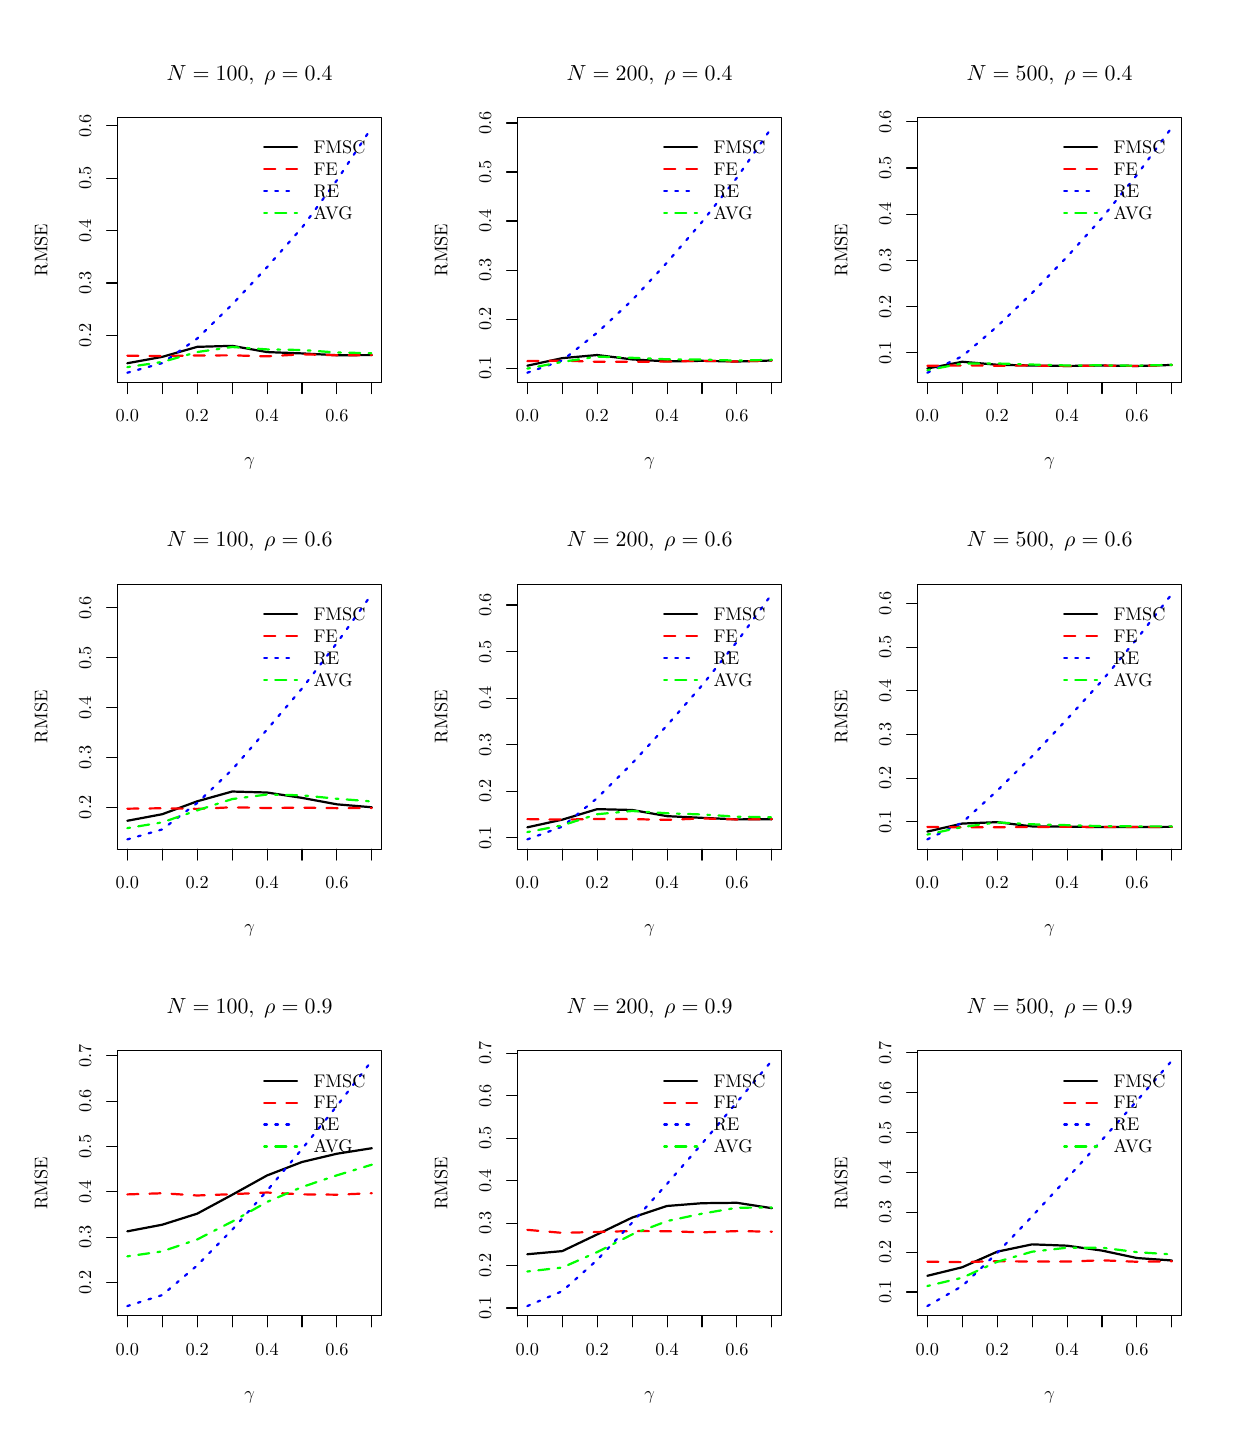
\begin{tikzpicture}[x=1pt,y=1pt]
\definecolor{fillColor}{RGB}{255,255,255}
\path[use as bounding box,fill=fillColor,fill opacity=0.00] (0,0) rectangle (433.62,505.89);
\begin{scope}
\path[clip] ( 32.47,377.65) rectangle (127.91,473.42);
\definecolor{drawColor}{RGB}{0,0,0}

\path[draw=drawColor,line width= 0.8pt,line join=round,line cap=round] ( 36.01,384.63) --
	( 48.63,386.93) --
	( 61.25,390.55) --
	( 73.88,390.91) --
	( 86.50,388.66) --
	( 99.13,388.18) --
	(111.75,387.53) --
	(124.37,387.57);
\end{scope}
\begin{scope}
\path[clip] (  0.00,  0.00) rectangle (433.62,505.89);
\definecolor{drawColor}{RGB}{0,0,0}

\path[draw=drawColor,line width= 0.4pt,line join=round,line cap=round] ( 36.01,377.65) -- (124.37,377.65);

\path[draw=drawColor,line width= 0.4pt,line join=round,line cap=round] ( 36.01,377.65) -- ( 36.01,373.69);

\path[draw=drawColor,line width= 0.4pt,line join=round,line cap=round] ( 48.63,377.65) -- ( 48.63,373.69);

\path[draw=drawColor,line width= 0.4pt,line join=round,line cap=round] ( 61.25,377.65) -- ( 61.25,373.69);

\path[draw=drawColor,line width= 0.4pt,line join=round,line cap=round] ( 73.88,377.65) -- ( 73.88,373.69);

\path[draw=drawColor,line width= 0.4pt,line join=round,line cap=round] ( 86.50,377.65) -- ( 86.50,373.69);

\path[draw=drawColor,line width= 0.4pt,line join=round,line cap=round] ( 99.13,377.65) -- ( 99.13,373.69);

\path[draw=drawColor,line width= 0.4pt,line join=round,line cap=round] (111.75,377.65) -- (111.75,373.69);

\path[draw=drawColor,line width= 0.4pt,line join=round,line cap=round] (124.37,377.65) -- (124.37,373.69);

\node[text=drawColor,anchor=base,inner sep=0pt, outer sep=0pt, scale=  0.66] at ( 36.01,363.40) {0.0};

\node[text=drawColor,anchor=base,inner sep=0pt, outer sep=0pt, scale=  0.66] at ( 61.25,363.40) {0.2};

\node[text=drawColor,anchor=base,inner sep=0pt, outer sep=0pt, scale=  0.66] at ( 86.50,363.40) {0.4};

\node[text=drawColor,anchor=base,inner sep=0pt, outer sep=0pt, scale=  0.66] at (111.75,363.40) {0.6};

\path[draw=drawColor,line width= 0.4pt,line join=round,line cap=round] ( 32.47,394.70) -- ( 32.47,470.39);

\path[draw=drawColor,line width= 0.4pt,line join=round,line cap=round] ( 32.47,394.70) -- ( 28.51,394.70);

\path[draw=drawColor,line width= 0.4pt,line join=round,line cap=round] ( 32.47,413.63) -- ( 28.51,413.63);

\path[draw=drawColor,line width= 0.4pt,line join=round,line cap=round] ( 32.47,432.55) -- ( 28.51,432.55);

\path[draw=drawColor,line width= 0.4pt,line join=round,line cap=round] ( 32.47,451.47) -- ( 28.51,451.47);

\path[draw=drawColor,line width= 0.4pt,line join=round,line cap=round] ( 32.47,470.39) -- ( 28.51,470.39);

\node[text=drawColor,rotate= 90.00,anchor=base,inner sep=0pt, outer sep=0pt, scale=  0.66] at ( 22.97,394.70) {0.2};

\node[text=drawColor,rotate= 90.00,anchor=base,inner sep=0pt, outer sep=0pt, scale=  0.66] at ( 22.97,413.63) {0.3};

\node[text=drawColor,rotate= 90.00,anchor=base,inner sep=0pt, outer sep=0pt, scale=  0.66] at ( 22.97,432.55) {0.4};

\node[text=drawColor,rotate= 90.00,anchor=base,inner sep=0pt, outer sep=0pt, scale=  0.66] at ( 22.97,451.47) {0.5};

\node[text=drawColor,rotate= 90.00,anchor=base,inner sep=0pt, outer sep=0pt, scale=  0.66] at ( 22.97,470.39) {0.6};

\path[draw=drawColor,line width= 0.4pt,line join=round,line cap=round] ( 32.47,377.65) --
	(127.91,377.65) --
	(127.91,473.42) --
	( 32.47,473.42) --
	( 32.47,377.65);
\end{scope}
\begin{scope}
\path[clip] (  0.00,337.26) rectangle (144.54,505.89);
\definecolor{drawColor}{RGB}{0,0,0}

\node[text=drawColor,anchor=base,inner sep=0pt, outer sep=0pt, scale=  0.79] at ( 80.19,486.92) {\bfseries $N=100, \;\rho=0.4$};

\node[text=drawColor,anchor=base,inner sep=0pt, outer sep=0pt, scale=  0.66] at ( 80.19,347.56) {$\gamma$};

\node[text=drawColor,rotate= 90.00,anchor=base,inner sep=0pt, outer sep=0pt, scale=  0.66] at (  7.13,425.53) {RMSE};
\end{scope}
\begin{scope}
\path[clip] ( 32.47,377.65) rectangle (127.91,473.42);
\definecolor{drawColor}{RGB}{255,0,0}

\path[draw=drawColor,line width= 0.8pt,dash pattern=on 4pt off 4pt ,line join=round,line cap=round] ( 36.01,387.35) --
	( 48.63,387.21) --
	( 61.25,387.43) --
	( 73.88,387.48) --
	( 86.50,387.12) --
	( 99.13,387.86) --
	(111.75,387.50) --
	(124.37,387.57);
\definecolor{drawColor}{RGB}{0,0,255}

\path[draw=drawColor,line width= 0.8pt,dash pattern=on 1pt off 3pt ,line join=round,line cap=round] ( 36.01,381.20) --
	( 48.63,384.68) --
	( 61.25,393.54) --
	( 73.88,405.84) --
	( 86.50,419.35) --
	( 99.13,433.63) --
	(111.75,450.76) --
	(124.37,469.87);
\definecolor{drawColor}{RGB}{0,255,0}

\path[draw=drawColor,line width= 0.8pt,dash pattern=on 1pt off 3pt on 4pt off 3pt ,line join=round,line cap=round] ( 36.01,383.22) --
	( 48.63,385.08) --
	( 61.25,388.67) --
	( 73.88,390.49) --
	( 86.50,389.63) --
	( 99.13,389.41) --
	(111.75,388.51) --
	(124.37,388.26);
\definecolor{drawColor}{RGB}{0,0,0}

\path[draw=drawColor,line width= 0.8pt,line join=round,line cap=round] ( 85.47,462.63) -- ( 97.35,462.63);
\definecolor{drawColor}{RGB}{255,0,0}

\path[draw=drawColor,line width= 0.8pt,dash pattern=on 4pt off 4pt ,line join=round,line cap=round] ( 85.47,454.71) -- ( 97.35,454.71);
\definecolor{drawColor}{RGB}{0,0,255}

\path[draw=drawColor,line width= 0.8pt,dash pattern=on 1pt off 3pt ,line join=round,line cap=round] ( 85.47,446.79) -- ( 97.35,446.79);
\definecolor{drawColor}{RGB}{0,255,0}

\path[draw=drawColor,line width= 0.8pt,dash pattern=on 1pt off 3pt on 4pt off 3pt ,line join=round,line cap=round] ( 85.47,438.87) -- ( 97.35,438.87);
\definecolor{drawColor}{RGB}{0,0,0}

\node[text=drawColor,anchor=base west,inner sep=0pt, outer sep=0pt, scale=  0.66] at (103.29,460.35) {FMSC};

\node[text=drawColor,anchor=base west,inner sep=0pt, outer sep=0pt, scale=  0.66] at (103.29,452.43) {FE};

\node[text=drawColor,anchor=base west,inner sep=0pt, outer sep=0pt, scale=  0.66] at (103.29,444.51) {RE};

\node[text=drawColor,anchor=base west,inner sep=0pt, outer sep=0pt, scale=  0.66] at (103.29,436.59) {AVG};
\end{scope}
\begin{scope}
\path[clip] (177.01,377.65) rectangle (272.45,473.42);
\definecolor{drawColor}{RGB}{0,0,0}

\path[draw=drawColor,line width= 0.8pt,line join=round,line cap=round] (180.55,383.74) --
	(193.17,386.47) --
	(205.79,387.60) --
	(218.42,386.01) --
	(231.04,385.30) --
	(243.67,385.50) --
	(256.29,385.25) --
	(268.91,385.62);
\end{scope}
\begin{scope}
\path[clip] (  0.00,  0.00) rectangle (433.62,505.89);
\definecolor{drawColor}{RGB}{0,0,0}

\path[draw=drawColor,line width= 0.4pt,line join=round,line cap=round] (180.55,377.65) -- (268.91,377.65);

\path[draw=drawColor,line width= 0.4pt,line join=round,line cap=round] (180.55,377.65) -- (180.55,373.69);

\path[draw=drawColor,line width= 0.4pt,line join=round,line cap=round] (193.17,377.65) -- (193.17,373.69);

\path[draw=drawColor,line width= 0.4pt,line join=round,line cap=round] (205.79,377.65) -- (205.79,373.69);

\path[draw=drawColor,line width= 0.4pt,line join=round,line cap=round] (218.42,377.65) -- (218.42,373.69);

\path[draw=drawColor,line width= 0.4pt,line join=round,line cap=round] (231.04,377.65) -- (231.04,373.69);

\path[draw=drawColor,line width= 0.4pt,line join=round,line cap=round] (243.67,377.65) -- (243.67,373.69);

\path[draw=drawColor,line width= 0.4pt,line join=round,line cap=round] (256.29,377.65) -- (256.29,373.69);

\path[draw=drawColor,line width= 0.4pt,line join=round,line cap=round] (268.91,377.65) -- (268.91,373.69);

\node[text=drawColor,anchor=base,inner sep=0pt, outer sep=0pt, scale=  0.66] at (180.55,363.40) {0.0};

\node[text=drawColor,anchor=base,inner sep=0pt, outer sep=0pt, scale=  0.66] at (205.79,363.40) {0.2};

\node[text=drawColor,anchor=base,inner sep=0pt, outer sep=0pt, scale=  0.66] at (231.04,363.40) {0.4};

\node[text=drawColor,anchor=base,inner sep=0pt, outer sep=0pt, scale=  0.66] at (256.29,363.40) {0.6};

\path[draw=drawColor,line width= 0.4pt,line join=round,line cap=round] (177.01,382.87) -- (177.01,471.44);

\path[draw=drawColor,line width= 0.4pt,line join=round,line cap=round] (177.01,382.87) -- (173.05,382.87);

\path[draw=drawColor,line width= 0.4pt,line join=round,line cap=round] (177.01,400.59) -- (173.05,400.59);

\path[draw=drawColor,line width= 0.4pt,line join=round,line cap=round] (177.01,418.30) -- (173.05,418.30);

\path[draw=drawColor,line width= 0.4pt,line join=round,line cap=round] (177.01,436.01) -- (173.05,436.01);

\path[draw=drawColor,line width= 0.4pt,line join=round,line cap=round] (177.01,453.72) -- (173.05,453.72);

\path[draw=drawColor,line width= 0.4pt,line join=round,line cap=round] (177.01,471.44) -- (173.05,471.44);

\node[text=drawColor,rotate= 90.00,anchor=base,inner sep=0pt, outer sep=0pt, scale=  0.66] at (167.51,382.87) {0.1};

\node[text=drawColor,rotate= 90.00,anchor=base,inner sep=0pt, outer sep=0pt, scale=  0.66] at (167.51,400.59) {0.2};

\node[text=drawColor,rotate= 90.00,anchor=base,inner sep=0pt, outer sep=0pt, scale=  0.66] at (167.51,418.30) {0.3};

\node[text=drawColor,rotate= 90.00,anchor=base,inner sep=0pt, outer sep=0pt, scale=  0.66] at (167.51,436.01) {0.4};

\node[text=drawColor,rotate= 90.00,anchor=base,inner sep=0pt, outer sep=0pt, scale=  0.66] at (167.51,453.72) {0.5};

\node[text=drawColor,rotate= 90.00,anchor=base,inner sep=0pt, outer sep=0pt, scale=  0.66] at (167.51,471.44) {0.6};

\path[draw=drawColor,line width= 0.4pt,line join=round,line cap=round] (177.01,377.65) --
	(272.45,377.65) --
	(272.45,473.42) --
	(177.01,473.42) --
	(177.01,377.65);
\end{scope}
\begin{scope}
\path[clip] (144.54,337.26) rectangle (289.08,505.89);
\definecolor{drawColor}{RGB}{0,0,0}

\node[text=drawColor,anchor=base,inner sep=0pt, outer sep=0pt, scale=  0.79] at (224.73,486.92) {\bfseries $N=200, \;\rho=0.4$};

\node[text=drawColor,anchor=base,inner sep=0pt, outer sep=0pt, scale=  0.66] at (224.73,347.56) {$\gamma$};

\node[text=drawColor,rotate= 90.00,anchor=base,inner sep=0pt, outer sep=0pt, scale=  0.66] at (151.67,425.53) {RMSE};
\end{scope}
\begin{scope}
\path[clip] (177.01,377.65) rectangle (272.45,473.42);
\definecolor{drawColor}{RGB}{255,0,0}

\path[draw=drawColor,line width= 0.8pt,dash pattern=on 4pt off 4pt ,line join=round,line cap=round] (180.55,385.40) --
	(193.17,385.57) --
	(205.79,385.17) --
	(218.42,385.16) --
	(231.04,385.24) --
	(243.67,385.50) --
	(256.29,385.25) --
	(268.91,385.62);
\definecolor{drawColor}{RGB}{0,0,255}

\path[draw=drawColor,line width= 0.8pt,dash pattern=on 1pt off 3pt ,line join=round,line cap=round] (180.55,381.20) --
	(193.17,385.62) --
	(205.79,395.66) --
	(218.42,407.39) --
	(231.04,421.03) --
	(243.67,435.69) --
	(256.29,451.67) --
	(268.91,469.87);
\definecolor{drawColor}{RGB}{0,255,0}

\path[draw=drawColor,line width= 0.8pt,dash pattern=on 1pt off 3pt on 4pt off 3pt ,line join=round,line cap=round] (180.55,382.69) --
	(193.17,385.12) --
	(205.79,387.03) --
	(218.42,386.59) --
	(231.04,386.06) --
	(243.67,385.95) --
	(256.29,385.57) --
	(268.91,385.86);
\definecolor{drawColor}{RGB}{0,0,0}

\path[draw=drawColor,line width= 0.8pt,line join=round,line cap=round] (230.01,462.63) -- (241.89,462.63);
\definecolor{drawColor}{RGB}{255,0,0}

\path[draw=drawColor,line width= 0.8pt,dash pattern=on 4pt off 4pt ,line join=round,line cap=round] (230.01,454.71) -- (241.89,454.71);
\definecolor{drawColor}{RGB}{0,0,255}

\path[draw=drawColor,line width= 0.8pt,dash pattern=on 1pt off 3pt ,line join=round,line cap=round] (230.01,446.79) -- (241.89,446.79);
\definecolor{drawColor}{RGB}{0,255,0}

\path[draw=drawColor,line width= 0.8pt,dash pattern=on 1pt off 3pt on 4pt off 3pt ,line join=round,line cap=round] (230.01,438.87) -- (241.89,438.87);
\definecolor{drawColor}{RGB}{0,0,0}

\node[text=drawColor,anchor=base west,inner sep=0pt, outer sep=0pt, scale=  0.66] at (247.83,460.35) {FMSC};

\node[text=drawColor,anchor=base west,inner sep=0pt, outer sep=0pt, scale=  0.66] at (247.83,452.43) {FE};

\node[text=drawColor,anchor=base west,inner sep=0pt, outer sep=0pt, scale=  0.66] at (247.83,444.51) {RE};

\node[text=drawColor,anchor=base west,inner sep=0pt, outer sep=0pt, scale=  0.66] at (247.83,436.59) {AVG};
\end{scope}
\begin{scope}
\path[clip] (321.55,377.65) rectangle (416.99,473.42);
\definecolor{drawColor}{RGB}{0,0,0}

\path[draw=drawColor,line width= 0.8pt,line join=round,line cap=round] (325.09,382.72) --
	(337.71,385.16) --
	(350.33,384.08) --
	(362.96,383.80) --
	(375.58,383.65) --
	(388.21,383.79) --
	(400.83,383.65) --
	(413.45,384.00);
\end{scope}
\begin{scope}
\path[clip] (  0.00,  0.00) rectangle (433.62,505.89);
\definecolor{drawColor}{RGB}{0,0,0}

\path[draw=drawColor,line width= 0.4pt,line join=round,line cap=round] (325.09,377.65) -- (413.45,377.65);

\path[draw=drawColor,line width= 0.4pt,line join=round,line cap=round] (325.09,377.65) -- (325.09,373.69);

\path[draw=drawColor,line width= 0.4pt,line join=round,line cap=round] (337.71,377.65) -- (337.71,373.69);

\path[draw=drawColor,line width= 0.4pt,line join=round,line cap=round] (350.33,377.65) -- (350.33,373.69);

\path[draw=drawColor,line width= 0.4pt,line join=round,line cap=round] (362.96,377.65) -- (362.96,373.69);

\path[draw=drawColor,line width= 0.4pt,line join=round,line cap=round] (375.58,377.65) -- (375.58,373.69);

\path[draw=drawColor,line width= 0.4pt,line join=round,line cap=round] (388.21,377.65) -- (388.21,373.69);

\path[draw=drawColor,line width= 0.4pt,line join=round,line cap=round] (400.83,377.65) -- (400.83,373.69);

\path[draw=drawColor,line width= 0.4pt,line join=round,line cap=round] (413.45,377.65) -- (413.45,373.69);

\node[text=drawColor,anchor=base,inner sep=0pt, outer sep=0pt, scale=  0.66] at (325.09,363.40) {0.0};

\node[text=drawColor,anchor=base,inner sep=0pt, outer sep=0pt, scale=  0.66] at (350.33,363.40) {0.2};

\node[text=drawColor,anchor=base,inner sep=0pt, outer sep=0pt, scale=  0.66] at (375.58,363.40) {0.4};

\node[text=drawColor,anchor=base,inner sep=0pt, outer sep=0pt, scale=  0.66] at (400.83,363.40) {0.6};

\path[draw=drawColor,line width= 0.4pt,line join=round,line cap=round] (321.55,388.42) -- (321.55,471.89);

\path[draw=drawColor,line width= 0.4pt,line join=round,line cap=round] (321.55,388.42) -- (317.59,388.42);

\path[draw=drawColor,line width= 0.4pt,line join=round,line cap=round] (321.55,405.11) -- (317.59,405.11);

\path[draw=drawColor,line width= 0.4pt,line join=round,line cap=round] (321.55,421.80) -- (317.59,421.80);

\path[draw=drawColor,line width= 0.4pt,line join=round,line cap=round] (321.55,438.50) -- (317.59,438.50);

\path[draw=drawColor,line width= 0.4pt,line join=round,line cap=round] (321.55,455.19) -- (317.59,455.19);

\path[draw=drawColor,line width= 0.4pt,line join=round,line cap=round] (321.55,471.89) -- (317.59,471.89);

\node[text=drawColor,rotate= 90.00,anchor=base,inner sep=0pt, outer sep=0pt, scale=  0.66] at (312.05,388.42) {0.1};

\node[text=drawColor,rotate= 90.00,anchor=base,inner sep=0pt, outer sep=0pt, scale=  0.66] at (312.05,405.11) {0.2};

\node[text=drawColor,rotate= 90.00,anchor=base,inner sep=0pt, outer sep=0pt, scale=  0.66] at (312.05,421.80) {0.3};

\node[text=drawColor,rotate= 90.00,anchor=base,inner sep=0pt, outer sep=0pt, scale=  0.66] at (312.05,438.50) {0.4};

\node[text=drawColor,rotate= 90.00,anchor=base,inner sep=0pt, outer sep=0pt, scale=  0.66] at (312.05,455.19) {0.5};

\node[text=drawColor,rotate= 90.00,anchor=base,inner sep=0pt, outer sep=0pt, scale=  0.66] at (312.05,471.89) {0.6};

\path[draw=drawColor,line width= 0.4pt,line join=round,line cap=round] (321.55,377.65) --
	(416.99,377.65) --
	(416.99,473.42) --
	(321.55,473.42) --
	(321.55,377.65);
\end{scope}
\begin{scope}
\path[clip] (289.08,337.26) rectangle (433.62,505.89);
\definecolor{drawColor}{RGB}{0,0,0}

\node[text=drawColor,anchor=base,inner sep=0pt, outer sep=0pt, scale=  0.79] at (369.27,486.92) {\bfseries $N=500, \;\rho=0.4$};

\node[text=drawColor,anchor=base,inner sep=0pt, outer sep=0pt, scale=  0.66] at (369.27,347.56) {$\gamma$};

\node[text=drawColor,rotate= 90.00,anchor=base,inner sep=0pt, outer sep=0pt, scale=  0.66] at (296.21,425.53) {RMSE};
\end{scope}
\begin{scope}
\path[clip] (321.55,377.65) rectangle (416.99,473.42);
\definecolor{drawColor}{RGB}{255,0,0}

\path[draw=drawColor,line width= 0.8pt,dash pattern=on 4pt off 4pt ,line join=round,line cap=round] (325.09,383.71) --
	(337.71,383.85) --
	(350.33,383.74) --
	(362.96,383.80) --
	(375.58,383.65) --
	(388.21,383.79) --
	(400.83,383.65) --
	(413.45,384.00);
\definecolor{drawColor}{RGB}{0,0,255}

\path[draw=drawColor,line width= 0.8pt,dash pattern=on 1pt off 3pt ,line join=round,line cap=round] (325.09,381.20) --
	(337.71,387.13) --
	(350.33,397.92) --
	(362.96,410.04) --
	(375.58,423.09) --
	(388.21,437.12) --
	(400.83,452.69) --
	(413.45,469.87);
\definecolor{drawColor}{RGB}{0,255,0}

\path[draw=drawColor,line width= 0.8pt,dash pattern=on 1pt off 3pt on 4pt off 3pt ,line join=round,line cap=round] (325.09,382.12) --
	(337.71,384.54) --
	(350.33,384.54) --
	(362.96,384.15) --
	(375.58,383.82) --
	(388.21,383.88) --
	(400.83,383.73) --
	(413.45,384.06);
\definecolor{drawColor}{RGB}{0,0,0}

\path[draw=drawColor,line width= 0.8pt,line join=round,line cap=round] (374.55,462.63) -- (386.43,462.63);
\definecolor{drawColor}{RGB}{255,0,0}

\path[draw=drawColor,line width= 0.8pt,dash pattern=on 4pt off 4pt ,line join=round,line cap=round] (374.55,454.71) -- (386.43,454.71);
\definecolor{drawColor}{RGB}{0,0,255}

\path[draw=drawColor,line width= 0.8pt,dash pattern=on 1pt off 3pt ,line join=round,line cap=round] (374.55,446.79) -- (386.43,446.79);
\definecolor{drawColor}{RGB}{0,255,0}

\path[draw=drawColor,line width= 0.8pt,dash pattern=on 1pt off 3pt on 4pt off 3pt ,line join=round,line cap=round] (374.55,438.87) -- (386.43,438.87);
\definecolor{drawColor}{RGB}{0,0,0}

\node[text=drawColor,anchor=base west,inner sep=0pt, outer sep=0pt, scale=  0.66] at (392.37,460.35) {FMSC};

\node[text=drawColor,anchor=base west,inner sep=0pt, outer sep=0pt, scale=  0.66] at (392.37,452.43) {FE};

\node[text=drawColor,anchor=base west,inner sep=0pt, outer sep=0pt, scale=  0.66] at (392.37,444.51) {RE};

\node[text=drawColor,anchor=base west,inner sep=0pt, outer sep=0pt, scale=  0.66] at (392.37,436.59) {AVG};
\end{scope}
\begin{scope}
\path[clip] ( 32.47,209.02) rectangle (127.91,304.79);
\definecolor{drawColor}{RGB}{0,0,0}

\path[draw=drawColor,line width= 0.8pt,line join=round,line cap=round] ( 36.01,219.30) --
	( 48.63,221.67) --
	( 61.25,226.33) --
	( 73.88,229.87) --
	( 86.50,229.51) --
	( 99.13,227.57) --
	(111.75,225.24) --
	(124.37,224.18);
\end{scope}
\begin{scope}
\path[clip] (  0.00,  0.00) rectangle (433.62,505.89);
\definecolor{drawColor}{RGB}{0,0,0}

\path[draw=drawColor,line width= 0.4pt,line join=round,line cap=round] ( 36.01,209.02) -- (124.37,209.02);

\path[draw=drawColor,line width= 0.4pt,line join=round,line cap=round] ( 36.01,209.02) -- ( 36.01,205.06);

\path[draw=drawColor,line width= 0.4pt,line join=round,line cap=round] ( 48.63,209.02) -- ( 48.63,205.06);

\path[draw=drawColor,line width= 0.4pt,line join=round,line cap=round] ( 61.25,209.02) -- ( 61.25,205.06);

\path[draw=drawColor,line width= 0.4pt,line join=round,line cap=round] ( 73.88,209.02) -- ( 73.88,205.06);

\path[draw=drawColor,line width= 0.4pt,line join=round,line cap=round] ( 86.50,209.02) -- ( 86.50,205.06);

\path[draw=drawColor,line width= 0.4pt,line join=round,line cap=round] ( 99.13,209.02) -- ( 99.13,205.06);

\path[draw=drawColor,line width= 0.4pt,line join=round,line cap=round] (111.75,209.02) -- (111.75,205.06);

\path[draw=drawColor,line width= 0.4pt,line join=round,line cap=round] (124.37,209.02) -- (124.37,205.06);

\node[text=drawColor,anchor=base,inner sep=0pt, outer sep=0pt, scale=  0.66] at ( 36.01,194.77) {0.0};

\node[text=drawColor,anchor=base,inner sep=0pt, outer sep=0pt, scale=  0.66] at ( 61.25,194.77) {0.2};

\node[text=drawColor,anchor=base,inner sep=0pt, outer sep=0pt, scale=  0.66] at ( 86.50,194.77) {0.4};

\node[text=drawColor,anchor=base,inner sep=0pt, outer sep=0pt, scale=  0.66] at (111.75,194.77) {0.6};

\path[draw=drawColor,line width= 0.4pt,line join=round,line cap=round] ( 32.47,224.14) -- ( 32.47,296.22);

\path[draw=drawColor,line width= 0.4pt,line join=round,line cap=round] ( 32.47,224.14) -- ( 28.51,224.14);

\path[draw=drawColor,line width= 0.4pt,line join=round,line cap=round] ( 32.47,242.16) -- ( 28.51,242.16);

\path[draw=drawColor,line width= 0.4pt,line join=round,line cap=round] ( 32.47,260.18) -- ( 28.51,260.18);

\path[draw=drawColor,line width= 0.4pt,line join=round,line cap=round] ( 32.47,278.20) -- ( 28.51,278.20);

\path[draw=drawColor,line width= 0.4pt,line join=round,line cap=round] ( 32.47,296.22) -- ( 28.51,296.22);

\node[text=drawColor,rotate= 90.00,anchor=base,inner sep=0pt, outer sep=0pt, scale=  0.66] at ( 22.97,224.14) {0.2};

\node[text=drawColor,rotate= 90.00,anchor=base,inner sep=0pt, outer sep=0pt, scale=  0.66] at ( 22.97,242.16) {0.3};

\node[text=drawColor,rotate= 90.00,anchor=base,inner sep=0pt, outer sep=0pt, scale=  0.66] at ( 22.97,260.18) {0.4};

\node[text=drawColor,rotate= 90.00,anchor=base,inner sep=0pt, outer sep=0pt, scale=  0.66] at ( 22.97,278.20) {0.5};

\node[text=drawColor,rotate= 90.00,anchor=base,inner sep=0pt, outer sep=0pt, scale=  0.66] at ( 22.97,296.22) {0.6};

\path[draw=drawColor,line width= 0.4pt,line join=round,line cap=round] ( 32.47,209.02) --
	(127.91,209.02) --
	(127.91,304.79) --
	( 32.47,304.79) --
	( 32.47,209.02);
\end{scope}
\begin{scope}
\path[clip] (  0.00,168.63) rectangle (144.54,337.26);
\definecolor{drawColor}{RGB}{0,0,0}

\node[text=drawColor,anchor=base,inner sep=0pt, outer sep=0pt, scale=  0.79] at ( 80.19,318.29) {\bfseries $N=100, \;\rho=0.6$};

\node[text=drawColor,anchor=base,inner sep=0pt, outer sep=0pt, scale=  0.66] at ( 80.19,178.93) {$\gamma$};

\node[text=drawColor,rotate= 90.00,anchor=base,inner sep=0pt, outer sep=0pt, scale=  0.66] at (  7.13,256.90) {RMSE};
\end{scope}
\begin{scope}
\path[clip] ( 32.47,209.02) rectangle (127.91,304.79);
\definecolor{drawColor}{RGB}{255,0,0}

\path[draw=drawColor,line width= 0.8pt,dash pattern=on 4pt off 4pt ,line join=round,line cap=round] ( 36.01,223.67) --
	( 48.63,223.82) --
	( 61.25,223.59) --
	( 73.88,224.18) --
	( 86.50,223.91) --
	( 99.13,224.03) --
	(111.75,223.86) --
	(124.37,223.92);
\definecolor{drawColor}{RGB}{0,0,255}

\path[draw=drawColor,line width= 0.8pt,dash pattern=on 1pt off 3pt ,line join=round,line cap=round] ( 36.01,212.57) --
	( 48.63,216.18) --
	( 61.25,225.73) --
	( 73.88,237.77) --
	( 86.50,252.27) --
	( 99.13,267.10) --
	(111.75,283.55) --
	(124.37,301.24);
\definecolor{drawColor}{RGB}{0,255,0}

\path[draw=drawColor,line width= 0.8pt,dash pattern=on 1pt off 3pt on 4pt off 3pt ,line join=round,line cap=round] ( 36.01,216.64) --
	( 48.63,218.73) --
	( 61.25,223.06) --
	( 73.88,227.14) --
	( 86.50,228.79) --
	( 99.13,228.50) --
	(111.75,227.26) --
	(124.37,226.28);
\definecolor{drawColor}{RGB}{0,0,0}

\path[draw=drawColor,line width= 0.8pt,line join=round,line cap=round] ( 85.47,294.00) -- ( 97.35,294.00);
\definecolor{drawColor}{RGB}{255,0,0}

\path[draw=drawColor,line width= 0.8pt,dash pattern=on 4pt off 4pt ,line join=round,line cap=round] ( 85.47,286.08) -- ( 97.35,286.08);
\definecolor{drawColor}{RGB}{0,0,255}

\path[draw=drawColor,line width= 0.8pt,dash pattern=on 1pt off 3pt ,line join=round,line cap=round] ( 85.47,278.16) -- ( 97.35,278.16);
\definecolor{drawColor}{RGB}{0,255,0}

\path[draw=drawColor,line width= 0.8pt,dash pattern=on 1pt off 3pt on 4pt off 3pt ,line join=round,line cap=round] ( 85.47,270.24) -- ( 97.35,270.24);
\definecolor{drawColor}{RGB}{0,0,0}

\node[text=drawColor,anchor=base west,inner sep=0pt, outer sep=0pt, scale=  0.66] at (103.29,291.72) {FMSC};

\node[text=drawColor,anchor=base west,inner sep=0pt, outer sep=0pt, scale=  0.66] at (103.29,283.80) {FE};

\node[text=drawColor,anchor=base west,inner sep=0pt, outer sep=0pt, scale=  0.66] at (103.29,275.88) {RE};

\node[text=drawColor,anchor=base west,inner sep=0pt, outer sep=0pt, scale=  0.66] at (103.29,267.96) {AVG};
\end{scope}
\begin{scope}
\path[clip] (177.01,209.02) rectangle (272.45,304.79);
\definecolor{drawColor}{RGB}{0,0,0}

\path[draw=drawColor,line width= 0.8pt,line join=round,line cap=round] (180.55,216.93) --
	(193.17,219.70) --
	(205.79,223.50) --
	(218.42,223.20) --
	(231.04,220.97) --
	(243.67,220.36) --
	(256.29,219.80) --
	(268.91,219.87);
\end{scope}
\begin{scope}
\path[clip] (  0.00,  0.00) rectangle (433.62,505.89);
\definecolor{drawColor}{RGB}{0,0,0}

\path[draw=drawColor,line width= 0.4pt,line join=round,line cap=round] (180.55,209.02) -- (268.91,209.02);

\path[draw=drawColor,line width= 0.4pt,line join=round,line cap=round] (180.55,209.02) -- (180.55,205.06);

\path[draw=drawColor,line width= 0.4pt,line join=round,line cap=round] (193.17,209.02) -- (193.17,205.06);

\path[draw=drawColor,line width= 0.4pt,line join=round,line cap=round] (205.79,209.02) -- (205.79,205.06);

\path[draw=drawColor,line width= 0.4pt,line join=round,line cap=round] (218.42,209.02) -- (218.42,205.06);

\path[draw=drawColor,line width= 0.4pt,line join=round,line cap=round] (231.04,209.02) -- (231.04,205.06);

\path[draw=drawColor,line width= 0.4pt,line join=round,line cap=round] (243.67,209.02) -- (243.67,205.06);

\path[draw=drawColor,line width= 0.4pt,line join=round,line cap=round] (256.29,209.02) -- (256.29,205.06);

\path[draw=drawColor,line width= 0.4pt,line join=round,line cap=round] (268.91,209.02) -- (268.91,205.06);

\node[text=drawColor,anchor=base,inner sep=0pt, outer sep=0pt, scale=  0.66] at (180.55,194.77) {0.0};

\node[text=drawColor,anchor=base,inner sep=0pt, outer sep=0pt, scale=  0.66] at (205.79,194.77) {0.2};

\node[text=drawColor,anchor=base,inner sep=0pt, outer sep=0pt, scale=  0.66] at (231.04,194.77) {0.4};

\node[text=drawColor,anchor=base,inner sep=0pt, outer sep=0pt, scale=  0.66] at (256.29,194.77) {0.6};

\path[draw=drawColor,line width= 0.4pt,line join=round,line cap=round] (177.01,213.14) -- (177.01,297.26);

\path[draw=drawColor,line width= 0.4pt,line join=round,line cap=round] (177.01,213.14) -- (173.05,213.14);

\path[draw=drawColor,line width= 0.4pt,line join=round,line cap=round] (177.01,229.96) -- (173.05,229.96);

\path[draw=drawColor,line width= 0.4pt,line join=round,line cap=round] (177.01,246.79) -- (173.05,246.79);

\path[draw=drawColor,line width= 0.4pt,line join=round,line cap=round] (177.01,263.61) -- (173.05,263.61);

\path[draw=drawColor,line width= 0.4pt,line join=round,line cap=round] (177.01,280.43) -- (173.05,280.43);

\path[draw=drawColor,line width= 0.4pt,line join=round,line cap=round] (177.01,297.26) -- (173.05,297.26);

\node[text=drawColor,rotate= 90.00,anchor=base,inner sep=0pt, outer sep=0pt, scale=  0.66] at (167.51,213.14) {0.1};

\node[text=drawColor,rotate= 90.00,anchor=base,inner sep=0pt, outer sep=0pt, scale=  0.66] at (167.51,229.96) {0.2};

\node[text=drawColor,rotate= 90.00,anchor=base,inner sep=0pt, outer sep=0pt, scale=  0.66] at (167.51,246.79) {0.3};

\node[text=drawColor,rotate= 90.00,anchor=base,inner sep=0pt, outer sep=0pt, scale=  0.66] at (167.51,263.61) {0.4};

\node[text=drawColor,rotate= 90.00,anchor=base,inner sep=0pt, outer sep=0pt, scale=  0.66] at (167.51,280.43) {0.5};

\node[text=drawColor,rotate= 90.00,anchor=base,inner sep=0pt, outer sep=0pt, scale=  0.66] at (167.51,297.26) {0.6};

\path[draw=drawColor,line width= 0.4pt,line join=round,line cap=round] (177.01,209.02) --
	(272.45,209.02) --
	(272.45,304.79) --
	(177.01,304.79) --
	(177.01,209.02);
\end{scope}
\begin{scope}
\path[clip] (144.54,168.63) rectangle (289.08,337.26);
\definecolor{drawColor}{RGB}{0,0,0}

\node[text=drawColor,anchor=base,inner sep=0pt, outer sep=0pt, scale=  0.79] at (224.73,318.29) {\bfseries $N=200, \;\rho=0.6$};

\node[text=drawColor,anchor=base,inner sep=0pt, outer sep=0pt, scale=  0.66] at (224.73,178.93) {$\gamma$};

\node[text=drawColor,rotate= 90.00,anchor=base,inner sep=0pt, outer sep=0pt, scale=  0.66] at (151.67,256.90) {RMSE};
\end{scope}
\begin{scope}
\path[clip] (177.01,209.02) rectangle (272.45,304.79);
\definecolor{drawColor}{RGB}{255,0,0}

\path[draw=drawColor,line width= 0.8pt,dash pattern=on 4pt off 4pt ,line join=round,line cap=round] (180.55,219.90) --
	(193.17,219.74) --
	(205.79,219.92) --
	(218.42,219.91) --
	(231.04,219.63) --
	(243.67,220.15) --
	(256.29,219.77) --
	(268.91,219.87);
\definecolor{drawColor}{RGB}{0,0,255}

\path[draw=drawColor,line width= 0.8pt,dash pattern=on 1pt off 3pt ,line join=round,line cap=round] (180.55,212.57) --
	(193.17,217.18) --
	(205.79,227.50) --
	(218.42,240.03) --
	(231.04,253.78) --
	(243.67,268.20) --
	(256.29,283.99) --
	(268.91,301.24);
\definecolor{drawColor}{RGB}{0,255,0}

\path[draw=drawColor,line width= 0.8pt,dash pattern=on 1pt off 3pt on 4pt off 3pt ,line join=round,line cap=round] (180.55,215.21) --
	(193.17,217.63) --
	(205.79,221.67) --
	(218.42,222.83) --
	(231.04,222.02) --
	(243.67,221.57) --
	(256.29,220.79) --
	(268.91,220.58);
\definecolor{drawColor}{RGB}{0,0,0}

\path[draw=drawColor,line width= 0.8pt,line join=round,line cap=round] (230.01,294.00) -- (241.89,294.00);
\definecolor{drawColor}{RGB}{255,0,0}

\path[draw=drawColor,line width= 0.8pt,dash pattern=on 4pt off 4pt ,line join=round,line cap=round] (230.01,286.08) -- (241.89,286.08);
\definecolor{drawColor}{RGB}{0,0,255}

\path[draw=drawColor,line width= 0.8pt,dash pattern=on 1pt off 3pt ,line join=round,line cap=round] (230.01,278.16) -- (241.89,278.16);
\definecolor{drawColor}{RGB}{0,255,0}

\path[draw=drawColor,line width= 0.8pt,dash pattern=on 1pt off 3pt on 4pt off 3pt ,line join=round,line cap=round] (230.01,270.24) -- (241.89,270.24);
\definecolor{drawColor}{RGB}{0,0,0}

\node[text=drawColor,anchor=base west,inner sep=0pt, outer sep=0pt, scale=  0.66] at (247.83,291.72) {FMSC};

\node[text=drawColor,anchor=base west,inner sep=0pt, outer sep=0pt, scale=  0.66] at (247.83,283.80) {FE};

\node[text=drawColor,anchor=base west,inner sep=0pt, outer sep=0pt, scale=  0.66] at (247.83,275.88) {RE};

\node[text=drawColor,anchor=base west,inner sep=0pt, outer sep=0pt, scale=  0.66] at (247.83,267.96) {AVG};
\end{scope}
\begin{scope}
\path[clip] (321.55,209.02) rectangle (416.99,304.79);
\definecolor{drawColor}{RGB}{0,0,0}

\path[draw=drawColor,line width= 0.8pt,line join=round,line cap=round] (325.09,215.39) --
	(337.71,218.29) --
	(350.33,218.80) --
	(362.96,217.26) --
	(375.58,217.17) --
	(388.21,217.02) --
	(400.83,217.03) --
	(413.45,217.11);
\end{scope}
\begin{scope}
\path[clip] (  0.00,  0.00) rectangle (433.62,505.89);
\definecolor{drawColor}{RGB}{0,0,0}

\path[draw=drawColor,line width= 0.4pt,line join=round,line cap=round] (325.09,209.02) -- (413.45,209.02);

\path[draw=drawColor,line width= 0.4pt,line join=round,line cap=round] (325.09,209.02) -- (325.09,205.06);

\path[draw=drawColor,line width= 0.4pt,line join=round,line cap=round] (337.71,209.02) -- (337.71,205.06);

\path[draw=drawColor,line width= 0.4pt,line join=round,line cap=round] (350.33,209.02) -- (350.33,205.06);

\path[draw=drawColor,line width= 0.4pt,line join=round,line cap=round] (362.96,209.02) -- (362.96,205.06);

\path[draw=drawColor,line width= 0.4pt,line join=round,line cap=round] (375.58,209.02) -- (375.58,205.06);

\path[draw=drawColor,line width= 0.4pt,line join=round,line cap=round] (388.21,209.02) -- (388.21,205.06);

\path[draw=drawColor,line width= 0.4pt,line join=round,line cap=round] (400.83,209.02) -- (400.83,205.06);

\path[draw=drawColor,line width= 0.4pt,line join=round,line cap=round] (413.45,209.02) -- (413.45,205.06);

\node[text=drawColor,anchor=base,inner sep=0pt, outer sep=0pt, scale=  0.66] at (325.09,194.77) {0.0};

\node[text=drawColor,anchor=base,inner sep=0pt, outer sep=0pt, scale=  0.66] at (350.33,194.77) {0.2};

\node[text=drawColor,anchor=base,inner sep=0pt, outer sep=0pt, scale=  0.66] at (375.58,194.77) {0.4};

\node[text=drawColor,anchor=base,inner sep=0pt, outer sep=0pt, scale=  0.66] at (400.83,194.77) {0.6};

\path[draw=drawColor,line width= 0.4pt,line join=round,line cap=round] (321.55,218.88) -- (321.55,297.86);

\path[draw=drawColor,line width= 0.4pt,line join=round,line cap=round] (321.55,218.88) -- (317.59,218.88);

\path[draw=drawColor,line width= 0.4pt,line join=round,line cap=round] (321.55,234.67) -- (317.59,234.67);

\path[draw=drawColor,line width= 0.4pt,line join=round,line cap=round] (321.55,250.47) -- (317.59,250.47);

\path[draw=drawColor,line width= 0.4pt,line join=round,line cap=round] (321.55,266.27) -- (317.59,266.27);

\path[draw=drawColor,line width= 0.4pt,line join=round,line cap=round] (321.55,282.06) -- (317.59,282.06);

\path[draw=drawColor,line width= 0.4pt,line join=round,line cap=round] (321.55,297.86) -- (317.59,297.86);

\node[text=drawColor,rotate= 90.00,anchor=base,inner sep=0pt, outer sep=0pt, scale=  0.66] at (312.05,218.88) {0.1};

\node[text=drawColor,rotate= 90.00,anchor=base,inner sep=0pt, outer sep=0pt, scale=  0.66] at (312.05,234.67) {0.2};

\node[text=drawColor,rotate= 90.00,anchor=base,inner sep=0pt, outer sep=0pt, scale=  0.66] at (312.05,250.47) {0.3};

\node[text=drawColor,rotate= 90.00,anchor=base,inner sep=0pt, outer sep=0pt, scale=  0.66] at (312.05,266.27) {0.4};

\node[text=drawColor,rotate= 90.00,anchor=base,inner sep=0pt, outer sep=0pt, scale=  0.66] at (312.05,282.06) {0.5};

\node[text=drawColor,rotate= 90.00,anchor=base,inner sep=0pt, outer sep=0pt, scale=  0.66] at (312.05,297.86) {0.6};

\path[draw=drawColor,line width= 0.4pt,line join=round,line cap=round] (321.55,209.02) --
	(416.99,209.02) --
	(416.99,304.79) --
	(321.55,304.79) --
	(321.55,209.02);
\end{scope}
\begin{scope}
\path[clip] (289.08,168.63) rectangle (433.62,337.26);
\definecolor{drawColor}{RGB}{0,0,0}

\node[text=drawColor,anchor=base,inner sep=0pt, outer sep=0pt, scale=  0.79] at (369.27,318.29) {\bfseries $N=500, \;\rho=0.6$};

\node[text=drawColor,anchor=base,inner sep=0pt, outer sep=0pt, scale=  0.66] at (369.27,178.93) {$\gamma$};

\node[text=drawColor,rotate= 90.00,anchor=base,inner sep=0pt, outer sep=0pt, scale=  0.66] at (296.21,256.90) {RMSE};
\end{scope}
\begin{scope}
\path[clip] (321.55,209.02) rectangle (416.99,304.79);
\definecolor{drawColor}{RGB}{255,0,0}

\path[draw=drawColor,line width= 0.8pt,dash pattern=on 4pt off 4pt ,line join=round,line cap=round] (325.09,217.08) --
	(337.71,216.92) --
	(350.33,216.99) --
	(362.96,217.01) --
	(375.58,217.16) --
	(388.21,217.02) --
	(400.83,217.03) --
	(413.45,217.11);
\definecolor{drawColor}{RGB}{0,0,255}

\path[draw=drawColor,line width= 0.8pt,dash pattern=on 1pt off 3pt ,line join=round,line cap=round] (325.09,212.57) --
	(337.71,218.66) --
	(350.33,230.16) --
	(362.96,242.63) --
	(375.58,256.01) --
	(388.21,269.91) --
	(400.83,285.04) --
	(413.45,301.24);
\definecolor{drawColor}{RGB}{0,255,0}

\path[draw=drawColor,line width= 0.8pt,dash pattern=on 1pt off 3pt on 4pt off 3pt ,line join=round,line cap=round] (325.09,214.32) --
	(337.71,217.03) --
	(350.33,218.72) --
	(362.96,218.03) --
	(375.58,217.72) --
	(388.21,217.35) --
	(400.83,217.27) --
	(413.45,217.27);
\definecolor{drawColor}{RGB}{0,0,0}

\path[draw=drawColor,line width= 0.8pt,line join=round,line cap=round] (374.55,294.00) -- (386.43,294.00);
\definecolor{drawColor}{RGB}{255,0,0}

\path[draw=drawColor,line width= 0.8pt,dash pattern=on 4pt off 4pt ,line join=round,line cap=round] (374.55,286.08) -- (386.43,286.08);
\definecolor{drawColor}{RGB}{0,0,255}

\path[draw=drawColor,line width= 0.8pt,dash pattern=on 1pt off 3pt ,line join=round,line cap=round] (374.55,278.16) -- (386.43,278.16);
\definecolor{drawColor}{RGB}{0,255,0}

\path[draw=drawColor,line width= 0.8pt,dash pattern=on 1pt off 3pt on 4pt off 3pt ,line join=round,line cap=round] (374.55,270.24) -- (386.43,270.24);
\definecolor{drawColor}{RGB}{0,0,0}

\node[text=drawColor,anchor=base west,inner sep=0pt, outer sep=0pt, scale=  0.66] at (392.37,291.72) {FMSC};

\node[text=drawColor,anchor=base west,inner sep=0pt, outer sep=0pt, scale=  0.66] at (392.37,283.80) {FE};

\node[text=drawColor,anchor=base west,inner sep=0pt, outer sep=0pt, scale=  0.66] at (392.37,275.88) {RE};

\node[text=drawColor,anchor=base west,inner sep=0pt, outer sep=0pt, scale=  0.66] at (392.37,267.96) {AVG};
\end{scope}
\begin{scope}
\path[clip] ( 32.47, 40.39) rectangle (127.91,136.16);
\definecolor{drawColor}{RGB}{0,0,0}

\path[draw=drawColor,line width= 0.8pt,line join=round,line cap=round] ( 36.01, 70.94) --
	( 48.63, 73.34) --
	( 61.25, 77.33) --
	( 73.88, 84.14) --
	( 86.50, 91.14) --
	( 99.13, 96.00) --
	(111.75, 98.99) --
	(124.37,100.98);
\end{scope}
\begin{scope}
\path[clip] (  0.00,  0.00) rectangle (433.62,505.89);
\definecolor{drawColor}{RGB}{0,0,0}

\path[draw=drawColor,line width= 0.4pt,line join=round,line cap=round] ( 36.01, 40.39) -- (124.37, 40.39);

\path[draw=drawColor,line width= 0.4pt,line join=round,line cap=round] ( 36.01, 40.39) -- ( 36.01, 36.43);

\path[draw=drawColor,line width= 0.4pt,line join=round,line cap=round] ( 48.63, 40.39) -- ( 48.63, 36.43);

\path[draw=drawColor,line width= 0.4pt,line join=round,line cap=round] ( 61.25, 40.39) -- ( 61.25, 36.43);

\path[draw=drawColor,line width= 0.4pt,line join=round,line cap=round] ( 73.88, 40.39) -- ( 73.88, 36.43);

\path[draw=drawColor,line width= 0.4pt,line join=round,line cap=round] ( 86.50, 40.39) -- ( 86.50, 36.43);

\path[draw=drawColor,line width= 0.4pt,line join=round,line cap=round] ( 99.13, 40.39) -- ( 99.13, 36.43);

\path[draw=drawColor,line width= 0.4pt,line join=round,line cap=round] (111.75, 40.39) -- (111.75, 36.43);

\path[draw=drawColor,line width= 0.4pt,line join=round,line cap=round] (124.37, 40.39) -- (124.37, 36.43);

\node[text=drawColor,anchor=base,inner sep=0pt, outer sep=0pt, scale=  0.66] at ( 36.01, 26.14) {0.0};

\node[text=drawColor,anchor=base,inner sep=0pt, outer sep=0pt, scale=  0.66] at ( 61.25, 26.14) {0.2};

\node[text=drawColor,anchor=base,inner sep=0pt, outer sep=0pt, scale=  0.66] at ( 86.50, 26.14) {0.4};

\node[text=drawColor,anchor=base,inner sep=0pt, outer sep=0pt, scale=  0.66] at (111.75, 26.14) {0.6};

\path[draw=drawColor,line width= 0.4pt,line join=round,line cap=round] ( 32.47, 52.46) -- ( 32.47,134.38);

\path[draw=drawColor,line width= 0.4pt,line join=round,line cap=round] ( 32.47, 52.46) -- ( 28.51, 52.46);

\path[draw=drawColor,line width= 0.4pt,line join=round,line cap=round] ( 32.47, 68.84) -- ( 28.51, 68.84);

\path[draw=drawColor,line width= 0.4pt,line join=round,line cap=round] ( 32.47, 85.23) -- ( 28.51, 85.23);

\path[draw=drawColor,line width= 0.4pt,line join=round,line cap=round] ( 32.47,101.61) -- ( 28.51,101.61);

\path[draw=drawColor,line width= 0.4pt,line join=round,line cap=round] ( 32.47,118.00) -- ( 28.51,118.00);

\path[draw=drawColor,line width= 0.4pt,line join=round,line cap=round] ( 32.47,134.38) -- ( 28.51,134.38);

\node[text=drawColor,rotate= 90.00,anchor=base,inner sep=0pt, outer sep=0pt, scale=  0.66] at ( 22.97, 52.46) {0.2};

\node[text=drawColor,rotate= 90.00,anchor=base,inner sep=0pt, outer sep=0pt, scale=  0.66] at ( 22.97, 68.84) {0.3};

\node[text=drawColor,rotate= 90.00,anchor=base,inner sep=0pt, outer sep=0pt, scale=  0.66] at ( 22.97, 85.23) {0.4};

\node[text=drawColor,rotate= 90.00,anchor=base,inner sep=0pt, outer sep=0pt, scale=  0.66] at ( 22.97,101.61) {0.5};

\node[text=drawColor,rotate= 90.00,anchor=base,inner sep=0pt, outer sep=0pt, scale=  0.66] at ( 22.97,118.00) {0.6};

\node[text=drawColor,rotate= 90.00,anchor=base,inner sep=0pt, outer sep=0pt, scale=  0.66] at ( 22.97,134.38) {0.7};

\path[draw=drawColor,line width= 0.4pt,line join=round,line cap=round] ( 32.47, 40.39) --
	(127.91, 40.39) --
	(127.91,136.16) --
	( 32.47,136.16) --
	( 32.47, 40.39);
\end{scope}
\begin{scope}
\path[clip] (  0.00,  0.00) rectangle (144.54,168.63);
\definecolor{drawColor}{RGB}{0,0,0}

\node[text=drawColor,anchor=base,inner sep=0pt, outer sep=0pt, scale=  0.79] at ( 80.19,149.66) {\bfseries $N=100, \;\rho=0.9$};

\node[text=drawColor,anchor=base,inner sep=0pt, outer sep=0pt, scale=  0.66] at ( 80.19, 10.30) {$\gamma$};

\node[text=drawColor,rotate= 90.00,anchor=base,inner sep=0pt, outer sep=0pt, scale=  0.66] at (  7.13, 88.27) {RMSE};
\end{scope}
\begin{scope}
\path[clip] ( 32.47, 40.39) rectangle (127.91,136.16);
\definecolor{drawColor}{RGB}{255,0,0}

\path[draw=drawColor,line width= 0.8pt,dash pattern=on 4pt off 4pt ,line join=round,line cap=round] ( 36.01, 84.29) --
	( 48.63, 84.71) --
	( 61.25, 83.90) --
	( 73.88, 84.37) --
	( 86.50, 84.97) --
	( 99.13, 84.31) --
	(111.75, 84.19) --
	(124.37, 84.72);
\definecolor{drawColor}{RGB}{0,0,255}

\path[draw=drawColor,line width= 0.8pt,dash pattern=on 1pt off 3pt ,line join=round,line cap=round] ( 36.01, 43.94) --
	( 48.63, 47.92) --
	( 61.25, 58.62) --
	( 73.88, 71.47) --
	( 86.50, 85.62) --
	( 99.13,100.70) --
	(111.75,116.27) --
	(124.37,132.61);
\definecolor{drawColor}{RGB}{0,255,0}

\path[draw=drawColor,line width= 0.8pt,dash pattern=on 1pt off 3pt on 4pt off 3pt ,line join=round,line cap=round] ( 36.01, 61.90) --
	( 48.63, 63.70) --
	( 61.25, 68.01) --
	( 73.88, 74.46) --
	( 86.50, 81.56) --
	( 99.13, 86.96) --
	(111.75, 91.19) --
	(124.37, 95.03);
\definecolor{drawColor}{RGB}{0,0,0}

\path[draw=drawColor,line width= 0.8pt,line join=round,line cap=round] ( 85.47,125.37) -- ( 97.35,125.37);
\definecolor{drawColor}{RGB}{255,0,0}

\path[draw=drawColor,line width= 0.8pt,dash pattern=on 4pt off 4pt ,line join=round,line cap=round] ( 85.47,117.45) -- ( 97.35,117.45);
\definecolor{drawColor}{RGB}{0,0,255}

\path[draw=drawColor,line width= 0.8pt,dash pattern=on 1pt off 3pt ,line join=round,line cap=round] ( 85.47,109.53) -- ( 97.35,109.53);
\definecolor{drawColor}{RGB}{0,255,0}

\path[draw=drawColor,line width= 0.8pt,dash pattern=on 1pt off 3pt on 4pt off 3pt ,line join=round,line cap=round] ( 85.47,101.61) -- ( 97.35,101.61);
\definecolor{drawColor}{RGB}{0,0,0}

\node[text=drawColor,anchor=base west,inner sep=0pt, outer sep=0pt, scale=  0.66] at (103.29,123.09) {FMSC};

\node[text=drawColor,anchor=base west,inner sep=0pt, outer sep=0pt, scale=  0.66] at (103.29,115.17) {FE};

\node[text=drawColor,anchor=base west,inner sep=0pt, outer sep=0pt, scale=  0.66] at (103.29,107.25) {RE};

\node[text=drawColor,anchor=base west,inner sep=0pt, outer sep=0pt, scale=  0.66] at (103.29, 99.33) {AVG};
\end{scope}
\begin{scope}
\path[clip] (177.01, 40.39) rectangle (272.45,136.16);
\definecolor{drawColor}{RGB}{0,0,0}

\path[draw=drawColor,line width= 0.8pt,line join=round,line cap=round] (180.55, 62.67) --
	(193.17, 63.80) --
	(205.79, 69.83) --
	(218.42, 75.91) --
	(231.04, 80.11) --
	(243.67, 81.11) --
	(256.29, 81.26) --
	(268.91, 79.31);
\end{scope}
\begin{scope}
\path[clip] (  0.00,  0.00) rectangle (433.62,505.89);
\definecolor{drawColor}{RGB}{0,0,0}

\path[draw=drawColor,line width= 0.4pt,line join=round,line cap=round] (180.55, 40.39) -- (268.91, 40.39);

\path[draw=drawColor,line width= 0.4pt,line join=round,line cap=round] (180.55, 40.39) -- (180.55, 36.43);

\path[draw=drawColor,line width= 0.4pt,line join=round,line cap=round] (193.17, 40.39) -- (193.17, 36.43);

\path[draw=drawColor,line width= 0.4pt,line join=round,line cap=round] (205.79, 40.39) -- (205.79, 36.43);

\path[draw=drawColor,line width= 0.4pt,line join=round,line cap=round] (218.42, 40.39) -- (218.42, 36.43);

\path[draw=drawColor,line width= 0.4pt,line join=round,line cap=round] (231.04, 40.39) -- (231.04, 36.43);

\path[draw=drawColor,line width= 0.4pt,line join=round,line cap=round] (243.67, 40.39) -- (243.67, 36.43);

\path[draw=drawColor,line width= 0.4pt,line join=round,line cap=round] (256.29, 40.39) -- (256.29, 36.43);

\path[draw=drawColor,line width= 0.4pt,line join=round,line cap=round] (268.91, 40.39) -- (268.91, 36.43);

\node[text=drawColor,anchor=base,inner sep=0pt, outer sep=0pt, scale=  0.66] at (180.55, 26.14) {0.0};

\node[text=drawColor,anchor=base,inner sep=0pt, outer sep=0pt, scale=  0.66] at (205.79, 26.14) {0.2};

\node[text=drawColor,anchor=base,inner sep=0pt, outer sep=0pt, scale=  0.66] at (231.04, 26.14) {0.4};

\node[text=drawColor,anchor=base,inner sep=0pt, outer sep=0pt, scale=  0.66] at (256.29, 26.14) {0.6};

\path[draw=drawColor,line width= 0.4pt,line join=round,line cap=round] (177.01, 43.26) -- (177.01,135.27);

\path[draw=drawColor,line width= 0.4pt,line join=round,line cap=round] (177.01, 43.26) -- (173.05, 43.26);

\path[draw=drawColor,line width= 0.4pt,line join=round,line cap=round] (177.01, 58.60) -- (173.05, 58.60);

\path[draw=drawColor,line width= 0.4pt,line join=round,line cap=round] (177.01, 73.93) -- (173.05, 73.93);

\path[draw=drawColor,line width= 0.4pt,line join=round,line cap=round] (177.01, 89.27) -- (173.05, 89.27);

\path[draw=drawColor,line width= 0.4pt,line join=round,line cap=round] (177.01,104.60) -- (173.05,104.60);

\path[draw=drawColor,line width= 0.4pt,line join=round,line cap=round] (177.01,119.93) -- (173.05,119.93);

\path[draw=drawColor,line width= 0.4pt,line join=round,line cap=round] (177.01,135.27) -- (173.05,135.27);

\node[text=drawColor,rotate= 90.00,anchor=base,inner sep=0pt, outer sep=0pt, scale=  0.66] at (167.51, 43.26) {0.1};

\node[text=drawColor,rotate= 90.00,anchor=base,inner sep=0pt, outer sep=0pt, scale=  0.66] at (167.51, 58.60) {0.2};

\node[text=drawColor,rotate= 90.00,anchor=base,inner sep=0pt, outer sep=0pt, scale=  0.66] at (167.51, 73.93) {0.3};

\node[text=drawColor,rotate= 90.00,anchor=base,inner sep=0pt, outer sep=0pt, scale=  0.66] at (167.51, 89.27) {0.4};

\node[text=drawColor,rotate= 90.00,anchor=base,inner sep=0pt, outer sep=0pt, scale=  0.66] at (167.51,104.60) {0.5};

\node[text=drawColor,rotate= 90.00,anchor=base,inner sep=0pt, outer sep=0pt, scale=  0.66] at (167.51,119.93) {0.6};

\node[text=drawColor,rotate= 90.00,anchor=base,inner sep=0pt, outer sep=0pt, scale=  0.66] at (167.51,135.27) {0.7};

\path[draw=drawColor,line width= 0.4pt,line join=round,line cap=round] (177.01, 40.39) --
	(272.45, 40.39) --
	(272.45,136.16) --
	(177.01,136.16) --
	(177.01, 40.39);
\end{scope}
\begin{scope}
\path[clip] (144.54,  0.00) rectangle (289.08,168.63);
\definecolor{drawColor}{RGB}{0,0,0}

\node[text=drawColor,anchor=base,inner sep=0pt, outer sep=0pt, scale=  0.79] at (224.73,149.66) {\bfseries $N=200, \;\rho=0.9$};

\node[text=drawColor,anchor=base,inner sep=0pt, outer sep=0pt, scale=  0.66] at (224.73, 10.30) {$\gamma$};

\node[text=drawColor,rotate= 90.00,anchor=base,inner sep=0pt, outer sep=0pt, scale=  0.66] at (151.67, 88.27) {RMSE};
\end{scope}
\begin{scope}
\path[clip] (177.01, 40.39) rectangle (272.45,136.16);
\definecolor{drawColor}{RGB}{255,0,0}

\path[draw=drawColor,line width= 0.8pt,dash pattern=on 4pt off 4pt ,line join=round,line cap=round] (180.55, 71.48) --
	(193.17, 70.39) --
	(205.79, 70.73) --
	(218.42, 71.05) --
	(231.04, 71.00) --
	(243.67, 70.58) --
	(256.29, 71.03) --
	(268.91, 70.83);
\definecolor{drawColor}{RGB}{0,0,255}

\path[draw=drawColor,line width= 0.8pt,dash pattern=on 1pt off 3pt ,line join=round,line cap=round] (180.55, 43.94) --
	(193.17, 49.33) --
	(205.79, 60.59) --
	(218.42, 74.08) --
	(231.04, 88.11) --
	(243.67,102.65) --
	(256.29,117.62) --
	(268.91,132.61);
\definecolor{drawColor}{RGB}{0,255,0}

\path[draw=drawColor,line width= 0.8pt,dash pattern=on 1pt off 3pt on 4pt off 3pt ,line join=round,line cap=round] (180.55, 56.43) --
	(193.17, 57.86) --
	(205.79, 63.45) --
	(218.42, 69.83) --
	(231.04, 74.65) --
	(243.67, 77.33) --
	(256.29, 79.48) --
	(268.91, 79.56);
\definecolor{drawColor}{RGB}{0,0,0}

\path[draw=drawColor,line width= 0.8pt,line join=round,line cap=round] (230.01,125.37) -- (241.89,125.37);
\definecolor{drawColor}{RGB}{255,0,0}

\path[draw=drawColor,line width= 0.8pt,dash pattern=on 4pt off 4pt ,line join=round,line cap=round] (230.01,117.45) -- (241.89,117.45);
\definecolor{drawColor}{RGB}{0,0,255}

\path[draw=drawColor,line width= 0.8pt,dash pattern=on 1pt off 3pt ,line join=round,line cap=round] (230.01,109.53) -- (241.89,109.53);
\definecolor{drawColor}{RGB}{0,255,0}

\path[draw=drawColor,line width= 0.8pt,dash pattern=on 1pt off 3pt on 4pt off 3pt ,line join=round,line cap=round] (230.01,101.61) -- (241.89,101.61);
\definecolor{drawColor}{RGB}{0,0,0}

\node[text=drawColor,anchor=base west,inner sep=0pt, outer sep=0pt, scale=  0.66] at (247.83,123.09) {FMSC};

\node[text=drawColor,anchor=base west,inner sep=0pt, outer sep=0pt, scale=  0.66] at (247.83,115.17) {FE};

\node[text=drawColor,anchor=base west,inner sep=0pt, outer sep=0pt, scale=  0.66] at (247.83,107.25) {RE};

\node[text=drawColor,anchor=base west,inner sep=0pt, outer sep=0pt, scale=  0.66] at (247.83, 99.33) {AVG};
\end{scope}
\begin{scope}
\path[clip] (321.55, 40.39) rectangle (416.99,136.16);
\definecolor{drawColor}{RGB}{0,0,0}

\path[draw=drawColor,line width= 0.8pt,line join=round,line cap=round] (325.09, 54.87) --
	(337.71, 57.97) --
	(350.33, 63.59) --
	(362.96, 66.24) --
	(375.58, 65.76) --
	(388.21, 63.99) --
	(400.83, 61.30) --
	(413.45, 60.42);
\end{scope}
\begin{scope}
\path[clip] (  0.00,  0.00) rectangle (433.62,505.89);
\definecolor{drawColor}{RGB}{0,0,0}

\path[draw=drawColor,line width= 0.4pt,line join=round,line cap=round] (325.09, 40.39) -- (413.45, 40.39);

\path[draw=drawColor,line width= 0.4pt,line join=round,line cap=round] (325.09, 40.39) -- (325.09, 36.43);

\path[draw=drawColor,line width= 0.4pt,line join=round,line cap=round] (337.71, 40.39) -- (337.71, 36.43);

\path[draw=drawColor,line width= 0.4pt,line join=round,line cap=round] (350.33, 40.39) -- (350.33, 36.43);

\path[draw=drawColor,line width= 0.4pt,line join=round,line cap=round] (362.96, 40.39) -- (362.96, 36.43);

\path[draw=drawColor,line width= 0.4pt,line join=round,line cap=round] (375.58, 40.39) -- (375.58, 36.43);

\path[draw=drawColor,line width= 0.4pt,line join=round,line cap=round] (388.21, 40.39) -- (388.21, 36.43);

\path[draw=drawColor,line width= 0.4pt,line join=round,line cap=round] (400.83, 40.39) -- (400.83, 36.43);

\path[draw=drawColor,line width= 0.4pt,line join=round,line cap=round] (413.45, 40.39) -- (413.45, 36.43);

\node[text=drawColor,anchor=base,inner sep=0pt, outer sep=0pt, scale=  0.66] at (325.09, 26.14) {0.0};

\node[text=drawColor,anchor=base,inner sep=0pt, outer sep=0pt, scale=  0.66] at (350.33, 26.14) {0.2};

\node[text=drawColor,anchor=base,inner sep=0pt, outer sep=0pt, scale=  0.66] at (375.58, 26.14) {0.4};

\node[text=drawColor,anchor=base,inner sep=0pt, outer sep=0pt, scale=  0.66] at (400.83, 26.14) {0.6};

\path[draw=drawColor,line width= 0.4pt,line join=round,line cap=round] (321.55, 49.03) -- (321.55,135.45);

\path[draw=drawColor,line width= 0.4pt,line join=round,line cap=round] (321.55, 49.03) -- (317.59, 49.03);

\path[draw=drawColor,line width= 0.4pt,line join=round,line cap=round] (321.55, 63.44) -- (317.59, 63.44);

\path[draw=drawColor,line width= 0.4pt,line join=round,line cap=round] (321.55, 77.84) -- (317.59, 77.84);

\path[draw=drawColor,line width= 0.4pt,line join=round,line cap=round] (321.55, 92.24) -- (317.59, 92.24);

\path[draw=drawColor,line width= 0.4pt,line join=round,line cap=round] (321.55,106.64) -- (317.59,106.64);

\path[draw=drawColor,line width= 0.4pt,line join=round,line cap=round] (321.55,121.05) -- (317.59,121.05);

\path[draw=drawColor,line width= 0.4pt,line join=round,line cap=round] (321.55,135.45) -- (317.59,135.45);

\node[text=drawColor,rotate= 90.00,anchor=base,inner sep=0pt, outer sep=0pt, scale=  0.66] at (312.05, 49.03) {0.1};

\node[text=drawColor,rotate= 90.00,anchor=base,inner sep=0pt, outer sep=0pt, scale=  0.66] at (312.05, 63.44) {0.2};

\node[text=drawColor,rotate= 90.00,anchor=base,inner sep=0pt, outer sep=0pt, scale=  0.66] at (312.05, 77.84) {0.3};

\node[text=drawColor,rotate= 90.00,anchor=base,inner sep=0pt, outer sep=0pt, scale=  0.66] at (312.05, 92.24) {0.4};

\node[text=drawColor,rotate= 90.00,anchor=base,inner sep=0pt, outer sep=0pt, scale=  0.66] at (312.05,106.64) {0.5};

\node[text=drawColor,rotate= 90.00,anchor=base,inner sep=0pt, outer sep=0pt, scale=  0.66] at (312.05,121.05) {0.6};

\node[text=drawColor,rotate= 90.00,anchor=base,inner sep=0pt, outer sep=0pt, scale=  0.66] at (312.05,135.45) {0.7};

\path[draw=drawColor,line width= 0.4pt,line join=round,line cap=round] (321.55, 40.39) --
	(416.99, 40.39) --
	(416.99,136.16) --
	(321.55,136.16) --
	(321.55, 40.39);
\end{scope}
\begin{scope}
\path[clip] (289.08,  0.00) rectangle (433.62,168.63);
\definecolor{drawColor}{RGB}{0,0,0}

\node[text=drawColor,anchor=base,inner sep=0pt, outer sep=0pt, scale=  0.79] at (369.27,149.66) {\bfseries $N=500, \;\rho=0.9$};

\node[text=drawColor,anchor=base,inner sep=0pt, outer sep=0pt, scale=  0.66] at (369.27, 10.30) {$\gamma$};

\node[text=drawColor,rotate= 90.00,anchor=base,inner sep=0pt, outer sep=0pt, scale=  0.66] at (296.21, 88.27) {RMSE};
\end{scope}
\begin{scope}
\path[clip] (321.55, 40.39) rectangle (416.99,136.16);
\definecolor{drawColor}{RGB}{255,0,0}

\path[draw=drawColor,line width= 0.8pt,dash pattern=on 4pt off 4pt ,line join=round,line cap=round] (325.09, 59.99) --
	(337.71, 59.81) --
	(350.33, 60.18) --
	(362.96, 60.02) --
	(375.58, 60.02) --
	(388.21, 60.48) --
	(400.83, 59.95) --
	(413.45, 60.12);
\definecolor{drawColor}{RGB}{0,0,255}

\path[draw=drawColor,line width= 0.8pt,dash pattern=on 1pt off 3pt ,line join=round,line cap=round] (325.09, 43.94) --
	(337.71, 51.17) --
	(350.33, 63.16) --
	(362.96, 76.38) --
	(375.58, 90.06) --
	(388.21,103.98) --
	(400.83,118.13) --
	(413.45,132.61);
\definecolor{drawColor}{RGB}{0,255,0}

\path[draw=drawColor,line width= 0.8pt,dash pattern=on 1pt off 3pt on 4pt off 3pt ,line join=round,line cap=round] (325.09, 51.18) --
	(337.71, 54.18) --
	(350.33, 59.93) --
	(362.96, 63.59) --
	(375.58, 65.03) --
	(388.21, 65.04) --
	(400.83, 63.42) --
	(413.45, 62.60);
\definecolor{drawColor}{RGB}{0,0,0}

\path[draw=drawColor,line width= 0.8pt,line join=round,line cap=round] (374.55,125.37) -- (386.43,125.37);
\definecolor{drawColor}{RGB}{255,0,0}

\path[draw=drawColor,line width= 0.8pt,dash pattern=on 4pt off 4pt ,line join=round,line cap=round] (374.55,117.45) -- (386.43,117.45);
\definecolor{drawColor}{RGB}{0,0,255}

\path[draw=drawColor,line width= 0.8pt,dash pattern=on 1pt off 3pt ,line join=round,line cap=round] (374.55,109.53) -- (386.43,109.53);
\definecolor{drawColor}{RGB}{0,255,0}

\path[draw=drawColor,line width= 0.8pt,dash pattern=on 1pt off 3pt on 4pt off 3pt ,line join=round,line cap=round] (374.55,101.61) -- (386.43,101.61);
\definecolor{drawColor}{RGB}{0,0,0}

\node[text=drawColor,anchor=base west,inner sep=0pt, outer sep=0pt, scale=  0.66] at (392.37,123.09) {FMSC};

\node[text=drawColor,anchor=base west,inner sep=0pt, outer sep=0pt, scale=  0.66] at (392.37,115.17) {FE};

\node[text=drawColor,anchor=base west,inner sep=0pt, outer sep=0pt, scale=  0.66] at (392.37,107.25) {RE};

\node[text=drawColor,anchor=base west,inner sep=0pt, outer sep=0pt, scale=  0.66] at (392.37, 99.33) {AVG};
\end{scope}
\end{tikzpicture}

  \caption{Random vs.\ Fixed effects estimator: $T=5, \sigma_{\varepsilon}^2 = 2.5$}
  \label{fig:REvsFE_T5}
\end{figure}

We see from Figures \ref{fig:REvsFE_T2} and \ref{fig:REvsFE_T5} that, regardless of the configuration of the other parameter values, there is always a range of values for $\gamma$ for which the random effects estimator has a smaller RMSE than the fixed effects estimator.
The width of this range increases as either the number of individuals $N$ or number of time periods $T$ decrease.
It also increases as the persistence $\rho$ of $x_{it}$ increases.
Indeed, when $N$ and $T$ are relatively small and $\rho$ is relatively large, the individual effects $\alpha_{i}$ can be \emph{strongly} correlated with $x_{it}$ and still result in a random effects estimator with a lower RMSE than the fixed effects estimator. 
The post-GFIC estimator essentially ``splits the difference'' between the random and fixed effects estimators.
While it cannot provide a uniform improvement over the fixed effects estimator, the post-GFIC estimator performs well.
When $\gamma$ is not too large it can yield a substantially lower RMSE than the fixed effects estimator.
The gains are particularly substantial when $x_{it}$ is relatively persistent and $T$ relatively small, as is common in micro-panel datasets.
The averaging estimator performs even better, providing a nearly uniform improvement over the post-GFIC estimator.
Only at very large values of $\gamma$ does it yield a higher RMSE, and these are points in the parameter space where the fixed effects, post-GFIC and averaging estimators are for all intents and purposes identical in RMSE.

\subsection{Dynamic Panel Example}
The details of this simulation are similar those of \cite{AndrewsLu}.\footnote{Unlike \cite{AndrewsLu} we do not generate ``extra'' presample observations for use with estimators that include a lagged dependent variable. This is for two reasons. First, in real-world applications such additional observations would not be available. Second, we are explicitly interested in how the loss of time periods for estimation affects finite sample MSE.} 
The simulated covariates and error terms are jointly normal with mean zero and unit variance. 
Specifically,
	\begin{equation}
	\label{eq:covar}
		\left[\begin{array}{c}
			x_{i}\\
			\eta_i\\
			v_{i}
	 \end{array} \right]\sim \mbox{iid}\; N\left(\left[\begin{array}{c}0_T\\ 0\\ 0_T \end{array}\right] ,\left[\begin{array}{ccc}
	 	 I_T & \sigma_{x\eta}\iota_T&\sigma_{xv}\Gamma_T \\
	 		\sigma_{x\eta}\iota_T'& 1&0_T' \\
	 		\sigma_{xv}\Gamma_T'& 0_T&  I_T
	 \end{array}\right]\right)
	\end{equation}
where $0_m$ denotes an $m$-vector of zeros, $I_m$ the $(m\times m)$ identity matrix, $\iota_m$ an $m$-vector of ones, and $\Gamma_m$ an $m\times m$ matrix with ones on the subdiagonal and zeros elsewhere, namely
	\begin{equation}
		\Gamma_m = \left[\begin{array}{cc}
	 	0_{m-1}' & 0\\
	 	I_{m-1} & 0_{m-1}
	 \end{array}\right].
	\end{equation}
Under this covariance matrix structure, $\eta_i$ and $v_{i}$ are uncorrelated with each other, but both are correlated with $x_{i}$: $E[x_{it}\eta_i]=\sigma_{x\eta}$ and $x_{it}$ is predetermined but not strictly exogenous with respect to $v_{it}$. Specifically, $E[x_{it}v_{it-1}]=\sigma_{xv}$, while $E[x_{it}v_{is}]=0$ for $s\neq t-1$. 

We initialize the presample observations $y_{i0}$ to zero, the mean of their stationary distribution, and generate the remaining time periods according to 
$$y_{it} = \gamma y_{it-1} + \theta x_{it} + \eta_i + v_{it}$$
In the simulation we take $\theta = 0.5$, $\sigma_{x\eta}=0.2$ and vary $\gamma$, $\sigma_{xv}$, $T$ and $N$ over a grid.
Each grid point is based on 2000 simulation replications.

The first question is how the finite sample MSE of the 2SLS estimators of $\theta$ based on specifications LW, LS, W, and S (see Section \ref{sec:panel}) changes with $\gamma$ and $\sigma_{xv}$. 
Figures \ref{fig:best} and \ref{fig:advantage} present RMSE comparisons for these four estimators over a simulation grid with $\gamma, \sigma_{xv} \in \{0, 0.005, 0.01, \hdots, 0.195, 0.2\}$, $N \in \{250,500\}$, $T \in \{4,5\}$.\footnote{Taking $T$ no smaller than 4 ensures that MSE exists for all four estimators: the finite sample moments of the 2SLS estimator only exist up to the order of over-identification.} 
For each point in the parameter space, the color in Figure \ref{fig:best} indicates the estimator of $\theta$ with the \emph{lowest} finite sample RMSE. 
The saturation of the color indicates the relative difference in RMSE of the best estimator at that point measured against the second-best estimator: darker indicates a larger advantage; lighter indicates a smaller advantage. 
While Figure  \ref{fig:best} indicates \emph{which} estimator is best, Figure \ref{fig:advantage} indicates how much of an advantage in RMSE can be gained over the correct specification, LW. 
These plots indicate that, provided $\gamma$ and $\sigma_{xv}$ are not too large, there are potentially large gains to be had by intentionally using an incorrectly specified estimator. 
The question remains, can the GFIC identify such situations?

%%%%%%%%%%%%%%%%%%%%%%%%%%%%%%%%%%%%%%%%
\begin{figure}
\centering
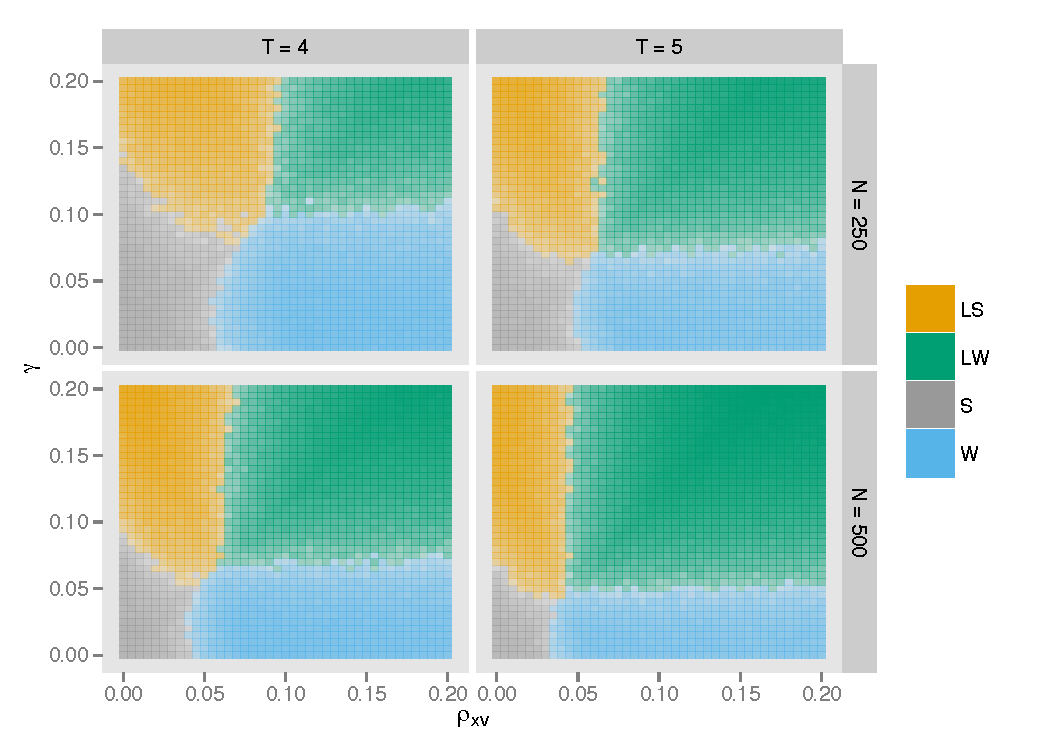
\includegraphics[scale = 0.8]{best_spec_vs_next_best}
\caption{ Minimum RMSE Specification at each combination of parameter values. Shading gives RMSE relative to second best specification.}
\label{fig:best}
\end{figure}

%%%%%%%%%%%%%%%%%%%%%%%%%%%%%%%%%%%%%%%%
\begin{figure}
\centering
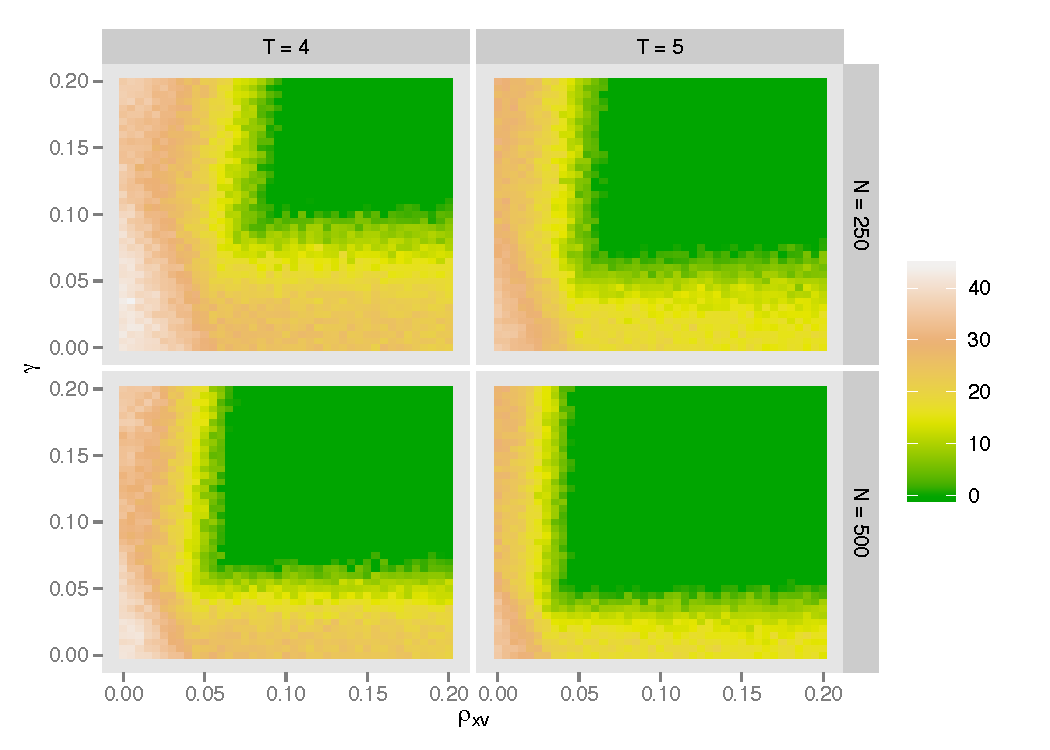
\includegraphics[scale = 0.8]{RMSE_advantage_vs_LW}
\caption{\% RMSE Advantage of Best Specification (vs.\ LW)}
\label{fig:advantage}
\end{figure}

%%%%%%%%%%%%%%%%%%%%%%%%%%%%%%%%%%%%%%%%

To provide a basis for comparison, we consider a number of other selection procedures. 
The first is a ``na\"{i}ve'' Downard J-test. 
To implement this procedure, we select the \emph{most restrictive} specification that is not rejected by the over-identifying restrictions test at a fixed significance level, either 5\% or 10\%. 
Specifically, we proceed as follows:
\begin{enumerate}
\item Use S unless the J-test rejects it. 
\item If S  is rejected, use W unless the J-test rejects it. 
\item If W is rejected, use LS unless the J-test rejects it. 
\item Only use LW if all others specifications are rejected.
\end{enumerate}
This procedure is ``na\"{i}ve'' because the significance thresholds are chosed arbitrarily rather than with a view towards some kind of selection optimality. 
We also consider the GMM model and moment selection criteria of \cite{AndrewsLu}: 
	\begin{eqnarray*}
	 \mbox{GMM-BIC} && J - (|c| - |b|) \log{n}\\
	 \mbox{GMM-AIC}&& J - 2(|c| - |b|)\\ 
	 \mbox{GMM-HQ} && J - 2.01 (|c| - |b|)  \log{\log{n}}
	\end{eqnarray*}
where $|b|$ is the number of parameters estimated, and $|c|$ the number of moment conditions used. 
Under certain assumptions, it can be shown that both the GMM-BIC and GMM-HQ are consistent: they select the maximal correctly specified estimator with probability approaching one in the limit. 
To implement these criteria, we calculate the J-test based on the optimal, two-step GMM estimator with a panel robust, heteroscedasticity-consistent, centered covariance matrix estimator for each specification.

To compare selection procedures we use the same simulation grid as above, namely $\gamma$ and $\sigma_{xv}$, namely $\gamma, \sigma_{xv} \in \{0, 0.005, 0.01, \hdots, 0.195, 0.20\}$.  
Again, each point on the simulation grid is calculated from 2000 simulation replications. 
Tables \ref{tab:rel} and \ref{tab:rmse} compare the performance of GFIC selection against each of the fixed specifications LW, LS, W, and S as well as the Downward J-test and the GMM moment and model selection criteria of \cite{AndrewsLu}. 
Table \ref{tab:rmse} gives average and maximum, i.e.\ worst-case, RMSE over the parameter space for $\gamma, \sigma_{xv}$ while Table \ref{tab:rel} gives \emph{relative} RMSE comparisons. Specifically, the values in the panel ``Average'' of Table \ref{tab:rel} tell how much larger, in percentage points, the average RMSE of a given estimator or selection procedure is than that of the pointwise oracle. 
The pointwise oracle is the infeasible procedure that uses the true minimum RMSE estimator at each point on the parameter grid. 
In contrast, the values in the panel ``Worst-Case'' of Table \ref{tab:rel} tell how much larger, in percentage points, the maximum RMSE of a given estimator or selection procedure is than that of the fixed specification LW. 
Over this parameter grid, LW is the minimax estimator.

Compared both to the fixed specifications and the other selection procedures, the GFIC performs well. 
In particular, it has a substantially lower average and worst-case RMSE than any of the other selection procedures.
Compared to simply using the correct specification, LW, the GFIC also performs relatively well. 
When $T$ and $N$ are small, the GFIC outperforms LW in average RMSE. 
As they grow it performs slightly worse, but only by a small amount.


\begin{table}[!tbp]
\begin{center}
\begin{tabular}{lrrrr}
\hline\hline
\multicolumn{1}{l}{Average}&\multicolumn{2}{c}{$N = 250$}&\multicolumn{2}{c}{$N = 500$}\\
&\multicolumn{1}{c}{$T=4$}&\multicolumn{1}{c}{$T=5$}&\multicolumn{1}{c}{$T=4$}&\multicolumn{1}{c}{$T=5$}\tabularnewline
\hline
LW&19&10&13& 7\tabularnewline
LS&30&44&54&79\tabularnewline
W&24&34&46&64\tabularnewline
S&31&50&64&94\tabularnewline
\hline
GFIC&17&13&15&10\tabularnewline
Downward J-test (10\%)&32&45&55&74\tabularnewline
Downward J-test (5\%)&31&47&57&79\tabularnewline
GMM-BIC&32&48&62&87\tabularnewline
GMM-HQ&32&46&57&77\tabularnewline
GMM-AIC&31&39&47&57\tabularnewline
\hline\\ \\ 

\hline\hline
\multicolumn{1}{l}{Worst-Case}&\multicolumn{2}{c}{$N = 250$}&\multicolumn{2}{c}{$N = 500$}\\
&\multicolumn{1}{c}{$T=4$}&\multicolumn{1}{c}{$T=5$}&\multicolumn{1}{c}{$T=4$}&\multicolumn{1}{c}{$T=5$}\tabularnewline
\hline
LW& 0& 0&  0&  0\tabularnewline
LS&42&81& 94&154\tabularnewline
W&49&88&105&158\tabularnewline
S&48&92&107&171\tabularnewline
\hline
GFIC& 3& 8&  6& 11\tabularnewline
Downward J-test (10\%)&43&78& 91&140\tabularnewline
Downward J-test (5\%)&45&83& 98&153\tabularnewline
GMM-BIC&48&89&106&168\tabularnewline
GMM-HQ&46&85&102&154\tabularnewline
GMM-AIC&39&68& 81&118\tabularnewline
\hline

\end{tabular}
\end{center}
\caption{Average and Worst-case RMSE Relative to Oracle (\% points)}
\label{tab:rel}
\end{table}

%%%%%%%%%%%%%%%%%%%%%%%%%%%%%%%%%%%%%%%%

\begin{table}[!tbp]
\begin{center}
\begin{tabular}{lrrrr}
\hline\hline
\multicolumn{1}{l}{Average}&\multicolumn{2}{c}{$N = 250$}&\multicolumn{2}{c}{$N = 500$}\\
&\multicolumn{1}{c}{$T=4$}&\multicolumn{1}{c}{$T=5$}&\multicolumn{1}{c}{$T=4$}&\multicolumn{1}{c}{$T=5$}\tabularnewline
\hline
LW&0.073&0.057&0.051&0.040\tabularnewline
LS&0.079&0.074&0.070&0.066\tabularnewline
W&0.075&0.069&0.066&0.061\tabularnewline
S&0.080&0.077&0.074&0.072\tabularnewline
\hline
GFIC&0.071&0.058&0.052&0.041\tabularnewline
Downward J-test (10\%)&0.080&0.074&0.070&0.065\tabularnewline
Downward J-test (5\%)&0.080&0.075&0.071&0.067\tabularnewline
GMM-BIC&0.080&0.076&0.073&0.069\tabularnewline
GMM-HQ&0.080&0.075&0.071&0.066\tabularnewline
GMM-AIC&0.080&0.071&0.066&0.058\tabularnewline
\hline\\ \\

\hline\hline
\multicolumn{1}{l}{Worst-Case}&\multicolumn{2}{c}{$N = 250$}&\multicolumn{2}{c}{$N = 500$}\\
&\multicolumn{1}{c}{$T=4$}&\multicolumn{1}{c}{$T=5$}&\multicolumn{1}{c}{$T=4$}&\multicolumn{1}{c}{$T=5$}\tabularnewline
\hline
LW&0.084&0.064&0.059&0.045\tabularnewline
LS&0.120&0.116&0.115&0.113\tabularnewline
W&0.125&0.120&0.122&0.115\tabularnewline
S&0.125&0.123&0.122&0.121\tabularnewline
\hline
GFIC&0.087&0.069&0.063&0.049\tabularnewline
Downward J-test (10\%)&0.120&0.114&0.113&0.107\tabularnewline
Downward J-test (5\%)&0.122&0.117&0.117&0.113\tabularnewline
GMM-BIC&0.125&0.121&0.122&0.119\tabularnewline
GMM-HQ&0.123&0.118&0.120&0.113\tabularnewline
GMM-AIC&0.117&0.107&0.107&0.097\tabularnewline
\hline
\end{tabular}
\end{center}
\caption{Average and Worst-case RMSE.}
\label{tab:rmse}
\end{table}
%%%%%%%%%%%%%%%%%%%%%%%%%%%%%%%%%%%%%%%%



%!TEX root = main.tex

\section{Conclusion}
\label{sec:conclude}
This paper has introduced the GFIC, a proposal to choose moment conditions and parameter restrictions based on the quality of the estimates they provide. 
The GFIC performs well in simulations for our dynamic panel example. 
While we focus here on applications to panel data, the GFIC can be applied to any GMM problem in which a minimal set of correctly specified moment conditions identifies an unrestricted model. 
A possible extension of this work would be to consider risk functions other than MSE, by analogy to \cite{ClaeskensCroux2006} and \cite{ClaeskensHjort2008}.
Another possibility would be to derive a version of the GFIC for GEL estimators. 
Although first-order equivalent to GMM, GEL estimators often exhibit superior finite-sample properties and may thus improve the quality of the selection criterion \citep{NeweySmith}. 


\newpage

\appendix
%!TEX root = main.tex

\subsection*{Results from Section \ref{sec:asymp}}

\begin{proof}[Proof of Theorem \ref{thm:asymp}]
By a mean-value expansion around $(\gamma_0,\theta_0)$,
	$$\sqrt{n}\left(\widehat{\beta}(b,c) - \beta_0^{(b)}\right) = - K(b,c)\Xi_c \sqrt{n} f_n(\gamma_0,\theta_0) + o_p(1)$$
and by the Lindeberg-Feller central limit theorem,
	$$\sqrt{n} f_n(\gamma_0,\theta_0) - \sqrt{n}E\left[f(Z_{ni},\gamma_0,\theta_0) \right]\overset{d}{\rightarrow} \left[\begin{array}{c} \mathscr{N}_g\\  \mathscr{N}_h\end{array}\right].$$
Now, by a mean-value expansion around $\gamma_n$,
	\begin{eqnarray*}
		\sqrt{n}E\left[ f(Z_{ni}, \gamma_0, \theta_0) \right] &=& \sqrt{n}E\left[ f(Z_{ni}, \gamma_n,\theta_0) \right] + \sqrt{n}\nabla_{\gamma'}E\left[ f(Z_{ni}, \bar{\gamma},\theta_0) \right] (\gamma_0 -\gamma_n)\\
			&=&\left[ \begin{array}{c} 0\\ \tau\end{array}\right] - \nabla_{\gamma'}E\left[ f(Z_{ni}, \bar{\gamma},\theta_0) \right] \delta\\
			&\rightarrow& \left[ \begin{array}{c} 0\\ \tau\end{array}\right] - F_\gamma\delta.
	\end{eqnarray*}
Hence,
	\begin{equation}
		\sqrt{n}f_n(\gamma_0, \theta_0) \overset{d}{\rightarrow} \left[\begin{array}{c} \mathscr{N}_g\\  \mathscr{N}_h\end{array}\right]+ \left[ \begin{array}{c} 0\\ \tau\end{array}\right] - F_\gamma\delta
	\end{equation}
and the result follows by the continuous mapping theorem.
\end{proof}

\begin{proof}[Proof of Corollary \ref{cor:valid}]
For the valid estimator,
	$$\Xi_c \left(\left[\begin{array}{c} \mathscr{N}_g\\  \mathscr{N}_h\end{array}\right]+ \left[ \begin{array}{c} 0\\ \tau\end{array}\right] - F_\gamma\delta\right) =  \mathscr{N}_g - G_\gamma \delta$$
since $\Xi_c$ picks out only components corresponding to $g$. Thus,
	$$\sqrt{n}\left( \widehat{\beta}_v - \beta_0 \right) \overset{d}{\rightarrow} -K_v\left(\mathscr{N}_g - G_\gamma \delta\right).$$
Finally
	\begin{eqnarray*}
		K_v G_\gamma \delta&=&  \left(\left[\begin{array}{c}G_\gamma' \\ G_\theta'\end{array}\right] W_{gg} \left[\begin{array}{cc} G_\gamma & G_\theta \end{array}\right] \right) \left[\begin{array}{c}G_\gamma' \\ G_\theta'\end{array}\right]W_{gg} G_\gamma\delta\\ \\
			&=& \left[\begin{array}{cc} 
				G_\gamma'W_{gg}G_\gamma & G_\gamma'W_{gg}G_\theta\\
				G_\theta'W_{gg}G_\gamma & G_\theta'W_{gg}G_\theta
			\end{array} \right]^{-1}
			\left[\begin{array}{c}
				G_\gamma'W_{gg}G_\gamma\\
				G_\theta'W_{gg}G_\gamma
			\end{array}\right]\delta =\left[\begin{array}{c} 0\\ \delta\end{array}\right]
	\end{eqnarray*}
by the definition of the matrix inverse.
\end{proof}


\subsection*{Results from Section \ref{sec:GFIC}}

\begin{proof}[Proof of Corollary \ref{cor:mulimit}]
   By a mean-value expansion around $\gamma_0$,
	\begin{eqnarray*}
		\mu_n  &=& \varphi(\gamma_0,\theta_0)+ \nabla_\gamma \varphi(\bar{\gamma},\theta_0)'(\gamma_n - \gamma_0)\\
			&=& \mu_0 + \nabla_\gamma \varphi(\bar{\gamma},\theta_0)' \delta/\sqrt{n}
	\end{eqnarray*}
for some $\bar{\gamma}$ between $\gamma_0$ and $\gamma_n = \gamma_0 +\delta/\sqrt{n}$. Hence,
	$$\sqrt{n}(\mu_n - \mu_0) = \nabla_\gamma \varphi(\bar{\gamma},\theta_0)' \delta \rightarrow \nabla_\gamma \varphi(\gamma_0,\theta_0)' \delta $$
The result follows since
$$\sqrt{n}\left(\widehat{\mu}(b,c) - \mu_n \right)  = \sqrt{n}\left( \widehat{\mu}(b,c) - \mu_0 \right) - \sqrt{n}\left(\mu_n - \mu_0\right).$$
\end{proof}


\begin{proof}[Proof of Corollary \ref{cor:muvalid}]
The result follows from Corollaries \ref{cor:valid} and \ref{cor:mulimit} since,
	\begin{eqnarray*}
		\sqrt{n}\left( \widehat{\mu}_v - \mu_n\right) &\overset{d}{\rightarrow}&\nabla_\beta\varphi_0' \left\{ \left[\begin{array}{c} 0\\ \delta \end{array}\right] -K_v\mathscr{N}_g  \right\}-\nabla_\gamma \varphi_0' \delta\\ 
			&=& -\nabla_\beta\varphi_0' K_v\mathscr{N}_g + \left[\begin{array}{cc} \nabla_\theta\varphi_0'  & \nabla_\gamma\varphi_0' \end{array}\right]\left[\begin{array}{c} 0\\ \delta\end{array}\right]-\nabla_\gamma \varphi_0' \delta\\
			&=& -\nabla_\beta(\gamma_0,\theta_0)' K_v\mathscr{N}_g.
	\end{eqnarray*}
\end{proof}


\begin{proof}[Proof of Lemma \ref{lem:tauhatasymp}]
By a mean-value expansion around $\beta_0 = ( \gamma_0', \theta_0')'$,
	$$\sqrt{n}h_n\left(\widehat{\beta}_v \right) = \sqrt{n}h_n(\beta_0) + H \sqrt{n} \left(\widehat{\beta}_v - \beta_0\right) + o_p(1).$$
Now, since
	$$\sqrt{n}f_n(\gamma_0,\theta_0) \overset{d}{\rightarrow} \left[\begin{array}{c} \mathscr{N}_g\\  \mathscr{N}_h\end{array}\right]+ \left[ \begin{array}{c} 0\\ \tau\end{array}\right] - \left[\begin{array}{c}G_\gamma\\ H_\gamma \end{array}\right]\delta$$
we have
	$$\sqrt{n}h_n(\gamma_0,\theta_0)\overset{d}{\rightarrow} \mathscr{N}_h + \tau - H_\gamma \delta.$$
Substituting, 
	\begin{eqnarray*}
		\sqrt{n}h_n(\widehat{\beta}_v) &\overset{d}{\rightarrow}&  \mathscr{N}_h + \tau - H_\gamma \delta+ H\left( -K_v \mathscr{N}_g + \left[\begin{array}{c} 0 \\ \delta \end{array} \right]\right)\\ 
			&=& \mathscr{N}_h + \tau - H_\gamma \delta - HK_v \mathscr{N}_g + \left[ \begin{array}{cc} H_\theta & H_\gamma \end{array}\right] \left[\begin{array}{c} 0 \\ \delta \end{array} \right]\\
			&=& \mathscr{N}_h  + \tau - H_\gamma \delta - HK_v \mathscr{N}_g  + H_\gamma \delta\\
			&=& \tau - HK_v \mathscr{N}_g + \mathscr{N}_h
	\end{eqnarray*}
as claimed.
\end{proof}

\begin{proof}[Proof of Corollary \ref{cor:biasestimators}]
Define
	$$\left[\begin{array}{c} U\\ V \end{array}\right]=\left[\begin{array}{c}\delta\\ \tau\end{array} \right] +\Psi\left[\begin{array}{c}\mathscr{N}_g \\ \mathscr{N}_h \end{array}\right].$$
By the Continuous Mapping Theorem and Theorem \ref{thm:jointbias},
	$$\left[\begin{array}{c} \widehat{\delta} \\ \widehat{\tau} \end{array}\right]\left[\begin{array}{cc} \widehat{\delta}' & \widehat{\tau}'\end{array} \right] \overset{d}{\rightarrow} \left[\begin{array}{c} U\\V \end{array}\right]\left[\begin{array}{cc}U' & V'\end{array} \right] $$
The result follows since
$$\Psi\Omega\Psi' =Var\left[\begin{array}{c}U\\V\end{array}\right] = 
E\left[\begin{array}{cc} 
				UU'&UV'\\
				VU'&VV'
				\end{array}\right] - 
				\left[\begin{array}{cc}
				\delta\delta'&\delta\tau'\\
				\tau\delta'&\tau\tau'
				\end{array}\right].$$
\end{proof}

\begin{proof}[Proof of Theorem \ref{thm:REvsFE}]
By expanding, we have 
\begin{align*}
&\sqrt{n} (\widehat{\beta}_{FE} - \beta) = A_n^{-1} \bigg ( n^{-1/2} \sum_{i=1}^n \mathbf{x}_i' Q \mathbf{v}_i  \bigg) \\
&\sqrt{n} (\widehat{\beta}_{RE} - \beta) = B_n \bigg (n^{-1/2} \sum_{i=1}^n \mathbf{x}_i' \widehat{\Omega}^{-1} \mathbf{v}_i  \bigg) \\
& \widehat{\tau} = \begin{bmatrix}
1 & \frac{-(T\widehat{\sigma}_\alpha^2 + \widehat{\sigma}_\epsilon^2)}{A_n B_n} 
\end{bmatrix} \begin{bmatrix}
n^{-1/2}(T\widehat{\sigma}_\alpha^2 + \widehat{\sigma}_\epsilon^2)\sum_{i=1}^n \mathbf{x}_i' \widehat{\Omega}^{-1} \mathbf{v}_i\\
n^{-1/2}\sum_{i=1}^n \mathbf{x}_i' Q \mathbf{v}_i
\end{bmatrix}
\end{align*}

where $A_n = \frac{1}{n} \sum_{i=1}^n \mathbf{x}_i' Q \mathbf{x}_i$ and $B_n = \big( \frac{1}{n} \sum_{i=1}^n \mathbf{x}_i' \widehat{\Omega}^{-1} \mathbf{x}_i \big)^{-1} $. The result follows, after some algebra, by applying the Lindeberg-Feller central limit theorem jointly to $n^{-1/2} \sum_{i=1}^n \mathbf{x}_i'Q\mathbf{v}_i$ and $n^{-1/2}\sum_{i=1}^n \mathbf{x}_i' \Omega^{-1} \mathbf{v}_i$. We also use that $\widehat{\Omega}$ is consistent estimator for $\Omega$ from an appropriate law of large numbers. Then, the joint distribution of $\widehat{\beta}_{RE}, \widehat{\beta}_{FE}$ and $\widehat{\tau}$ is derived to be

\[
 \begin{bmatrix}
\sqrt{n} (\widehat{\beta}_{RE} - \beta)\\
\sqrt{n} (\widehat{\beta}_{FE} - \beta)\\
\widehat{\tau}
\end{bmatrix} \rightarrow_d  \begin{bmatrix}
\frac{B}{T\sigma_\alpha^2 + \sigma_\epsilon^2} & 0 \\
0 & A^{-1} \\
1 & \frac{-(T\sigma_\alpha^2 + \sigma_\epsilon^2)}{AB}\\
\end{bmatrix} \bigg(\begin{bmatrix}
\tau\\
0
\end{bmatrix}   + M  \bigg)\\
\]


where $ A = E[\mathbf{x}_i' Q \mathbf{x}_i], B=E[\mathbf{x_i}' \Omega^{-1} \mathbf{x}_i]^{-1}$, and  $M \sim N(0, \widetilde{V}),$ with

\[
\widetilde{V} =  \begin{bmatrix}
(T\sigma_\alpha^2 + \sigma_\epsilon^2)^2 E[\mathbf{x}_i' \Omega^{-1} \mathbf{x}_i] & (T\sigma_\alpha^2 + \sigma_\epsilon^2) E[\mathbf{x}_i' Q \mathbf{x}_i] \\
 (T\sigma_\alpha^2 + \sigma_\epsilon^2) E[\mathbf{x}_i' Q \mathbf{x}_i] & \sigma_\epsilon^2 E[\mathbf{x}_i' Q \mathbf{x}_i]
\end{bmatrix}. \\
\]

\end{proof}

\begin{proof}[Proof of Theorem \ref{thm:limitDpanel}.]
  This proof is standard, so we provide only a sketch.
Expanding, 
\begin{align*}
  \sqrt{n}\left[\widehat{\beta}(k,\cdot) - \beta\right] &=(0, \mathbf{0}_{k-1}', \delta)' + \widehat{Q}(k,\cdot)\left[ n^{-1/2}Z'(k,\cdot)\Delta \mathbf{v}\right]\\
  \sqrt{n}\left[\widehat{\beta}(r,\cdot) - \beta_{r}\right] &=  \widehat{Q}(r,\cdot)\left\{ \delta \left[n^{-1}Z'(r,\cdot) L^{k}\Delta \mathbf{y}^+\right] + \left[n^{-1/2}Z'(r,\cdot)\Delta \mathbf{v}^{+}\right] \right\}
\end{align*}
The result follows, after some algebra, by applying the Lindeberg-Feller central limit theorem to $n^{-1/2}Z'(k,\cdot)\Delta \mathbf{v}$ and $n^{-1/2}Z'(r,\cdot)\Delta \mathbf{v}^{+}$ and an appropriate law of large numbers to $n^{-1} Z'(r,\cdot)L^k \Delta \mathbf{y}^{+}$, where $(\cdot)$ is either $\text{P}$ or $\text{S}$ depending on the instrument set used.
\end{proof}


\begin{proof}[Proof of Theorem \ref{thm:DpanelJoint}]
  Expanding $\widehat{\beta}(k,\text{P})$ from Equation \ref{eq:DpanelEstimators} 
  \begin{align*}
    n^{-1/2}X'\left[ \Delta \mathbf{y} - W(k)\widehat{\beta}(k,\text{P})  \right] 
    %&= n^{-1/2}X'\left\{ \left[W(k) \beta_n + \Delta \mathbf{v}\right] - W(k) \left[ \beta_n + \widehat{Q}(k,\text{P}) n^{-1} Z'(k,\text{P})\Delta \mathbf{v} \right] \right\} \\
    &= n^{-1/2}X'\left[ \Delta \mathbf{v}  - W(k)\, \widehat{Q}(k,\text{P}) \, n^{-1} Z'(k,\text{P})\Delta \mathbf{v}\right] \\
    %&= n^{-1/2}X'\Delta \mathbf{v}  - n^{-1}X'W(k)\,\widehat{Q}(k,\text{P})\left[ n^{-1/2} Z'(k,\text{P})\Delta \mathbf{v}\right]\\
    &= \left[
    \begin{array}{cc}
      -n^{-1} X'W(k) \, \widehat{Q}(k,\text{P}) & I_{T-k-1}
    \end{array}
  \right] 
  \left[
  \begin{array}{c}
    n^{-1/2}Z'(k,\text{P}) \Delta \mathbf{v} \\
    n^{-1/2} X' \Delta \mathbf{v}
  \end{array}
\right]
  \end{align*}
  using $\Delta \mathbf{y} = W(k) \beta_n + \Delta \mathbf{v}$. 
  Similarly, expanding $\widehat{\beta}(k,\text{P})$ from Equation \ref{eq:DpanelEstimators},
  \[
    \sqrt{n}\left[ \widehat{\beta}(k,\text{P}) \right] = \left[
    \begin{array}{ccc}
      0 & \mathbf{0}_{k-1} & \delta  
    \end{array}
  \right] + \widehat{Q}(k,\text{P}) n^{-1/2}Z'(k,\text{P}) \Delta \mathbf{v}
  \]
  and since $\widehat{\delta}$ is $\sqrt{n}$ times the $k$\textsuperscript{th} element of $\widehat{\beta}(k,\text{P})$ and the $k$\textsuperscript{th} element $\beta$ is zero, we have
  \[
    \widehat{\delta} = \delta + \left[
    \begin{array}{ccc}
    0 & \mathbf{0}'_{k-1} & 1  
    \end{array}
  \right] \widehat{Q}(k,\text{P}) n^{-1/2} Z'(k,\text{P})\Delta \mathbf{v}.
  \]
  By a law of large numbers $\widehat{Q}(k,\text{P}) \rightarrow_p Q(k,\text{P})$ and $n^{-1}X'W(k) \rightarrow_p \boldsymbol{\xi}' \otimes \boldsymbol{\iota}_{T-k-1}$, hence 
  \[
    \left[
    \begin{array}{c}
      \widehat{\delta} - \delta \\ \widehat{\tau}
    \end{array}
  \right] = \Psi
  \left[
  \begin{array}{c}
    n^{-1/2}Z'(k,\text{P}) \Delta \mathbf{v} \\
    n^{-1/2} X' \Delta \mathbf{v}
  \end{array}
\right] + o_p(1).
  \]
  The result follows, after some algebra, by applying the Lindeberg-Feller central limit theorem jointly to $n^{-1/2}Z'(k,\text{P})\Delta\mathbf{v}$ and $n^{-1/2}X'\Delta \mathbf{v}$ and noting that the permutation matrix $\Pi$ maps the vector $[n^{-1/2}Z'(k,\text{S})\Delta \mathbf{v}]$ to the vector $\left[
  \begin{array}{cc}
    \left\{n^{-1/2} Z'(k,P)\Delta \mathbf{v}\right\}' &
    \left\{n^{-1/2} X'\Delta \mathbf{v}\right\}' 
  \end{array}
\right]'.$
\end{proof}




%\singlespacing
%References

\bibliographystyle{elsarticle-harv}
\bibliography{GFIC_refs}

\end{document}
